\documentclass[10pt]{beamer}

\usepackage{xeCJK}
\setCJKmainfont{Noto Sans CJK SC}
\xeCJKsetup{PunctStyle=kaiming,CJKspace=true,CheckSingle=true} 

\DeclareGraphicsRule{*}{mps}{*}{}
\usepackage{subfigure}
\usepackage{amssymb, amsmath, amsfonts,verbatim}
\usepackage{tikz}
\graphicspath{ {./} }
\usetikzlibrary{matrix,arrows,fit,backgrounds,mindmap,plotmarks,decorations.pathreplacing}
\usepackage{tkz-euclide}
\usepackage{pgfplots}
\pgfplotsset{compat=1.12}
\pgfdeclarelayer{background}
\pgfsetlayers{background,main}

\tikzset{decoration={name=none},}

\usepackage{esvect}
\usetikzlibrary{circuits}
\usetikzlibrary{intersections} 
\newlength\figureheight
\newlength\figurewidth

\newcommand{\tikzdir}[1]{#1.tikz}
\newcommand{\inputtikz}[1]{\input{\tikzdir{#1}}}

\newcommand{\tI}{\tilde {\mathcal I}}
\newcommand{\tA}{\tilde A}
\newcommand{\ty}{\tilde y}
\newcommand{\tx}{\tilde x}
\newcommand{\tw}{\tilde w}
\newcommand{\tv}{\tilde v}
\newcommand{\tC}{\tilde C}
\newcommand{\tP}{\tilde P}
\newcommand{\Ic}{{\mathcal I^c}}
\newcommand{\J}{{\mathcal J}}
\newcommand{\K}{{\mathcal K}}

\newcommand{\diag}{\text{diag}}
\DeclareMathOperator{\1}{\textbf{1}}

\DeclareMathOperator{\Smin}{Smin}
\DeclareMathOperator{\Smid}{Smid}
\DeclareMathOperator{\Smax}{Smax}
\DeclareMathOperator{\MSE}{MSE}
\DeclareMathOperator{\rank}{rank}
\DeclareMathOperator{\Med}{Med}
\DeclareMathOperator{\Max}{Max}
\DeclareMathOperator{\Min}{Min}
\DeclareMathOperator{\tr}{tr}
\DeclareMathOperator{\Cov}{Cov}
\DeclareMathOperator{\logdet}{log\;det}
\DeclareMathOperator{\argmin}{arg\;min}
\DeclareMathOperator{\argmax}{arg\;max}
\let\Tiny\tiny

\DeclareMathOperator{\E}{\mathbb E}
\tikzstyle{sensor} = [draw, fill=blue!20, rectangle, rounded corners,
minimum height=2em, minimum width=7em]
\tikzstyle{est} = [draw, fill=orange!20, rectangle, rounded corners,
minimum height=2em, minimum width=7em]
\tikzstyle{pinstyle} = [pin edge={to-,thin,black}]


\title[Kalman Filter]{A Distributed Estimator Design via Decomposing Steady-State Kalman Filter}
\author[Yilin Mo]{Yilin Mo}
\institute[Tsinghua]{Department of Automation, Tsinghua University}
\date[May 29, 2021]{YAC 2021}

\usetheme[block=fill]{metropolis}
\definecolor{thupurple}{RGB}{102,8,116}
\definecolor{caltechcolor}{RGB}{102,8,116}
\setbeamercolor{title separator}{fg=black!50}
\setbeamercolor{frametitle}{bg=thupurple!70!black}

\begin{document}

\begin{frame}
  \titlepage
\end{frame}

%\frame{\tableofcontents}

\section{Introduction}

\begin{frame}{Motivation}
  \begin{itemize}
    \item Sensor Networks are becoming ubiquitous, with lots of interesting applications.
      \begin{itemize}
	\item environmental monitoring
	\item health care
	\item industrial monitoring
	\item military applications (threat detection)
	\item \ldots
      \end{itemize}
    \item {\bf Low cost} nodes with {\bf limited energy budget} and {\bf limited communication capability}.
    \item Communication is unreliable. 
    \item Communication costs too much resources (energy, bandwidth). 
    \item Sensor may be compromised.
    \item \ldots
    \item \bf How to do information fusion in sensor network?
  \end{itemize}
\end{frame}

\section{Decomposing Steady-State Kalman Filter }

\begin{frame}{LTI System}
  Consider the following LTI(Linear Time-Invariant) system:
  \begin{block}{System Description}
    \begin{displaymath}
	x(k+1) = A x(k) + w(k),\, y(k) = C x(k) + v(k).
    \end{displaymath}
  \end{block}
  \begin{itemize}
    \item $x(k) \in \mathbb R^n$ is the state at time $k$.
    \item  $y(k) \in \mathbb R^m$ is the measurements from the sensors. 
    \item $w(k),v(k),x(0)$ are independent Gaussian random variables, and $x(0) \sim \mathcal N(\bar x,\;\Sigma)$, $w(k) \sim \mathcal N(0,\;Q)$ and $v(k) \sim \mathcal N(0,\;R)$. 
  \end{itemize}
\end{frame}

\begin{frame}{Kalman Filter}
  Kalman filter takes the following form:
  \begin{align*}
    Prediction:&&\\
	       &\hat x^-(k + 1)  = A \hat x(k)  , \quad P^-(k + 1)  = AP(k) A'  + Q ,\\
    Correction:&&\\
	       &\hat x(k) = \hat x^-(k)  + P^-(k) C'(CP^-(k) C'+R)^{-1} (y(k)  - C \hat x(k) ) , \\
	       &P(k) = \left[(P^-(k))^{-1} + C' R^{-1} C \right]^{-1},
  \end{align*}
  with initial condition
  \begin{displaymath}
    \hat x^-(0)  = \bar x_0 ,\quad P^-(0)  = \Sigma.
  \end{displaymath}
\end{frame}

\begin{frame}{Steady State Kalman Filter}
  \begin{itemize}
    \item In practice, the Kalman gain converges to a fixed value exponentially fast.
    \item Kalman filter in steady state:
      \begin{align}
	\hat x(k+1) = A \hat x(k) + K(y(k+1)-CA\hat x(k)),
      \end{align}
      where $K$ is the steady state (asymptotic) Kalman gain, and $A-KCA$ is stable.
      \begin{center}
	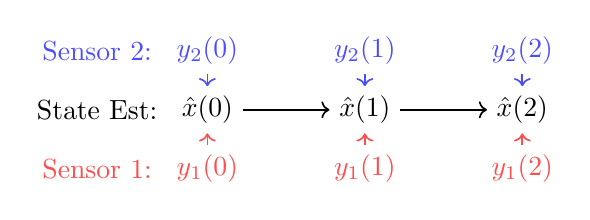
\begin{tikzpicture}[x=2cm, y=0.75cm]
	  \node at (-0.7,0) {State Est:};
	  \node [blue!70] at (-0.7,1) {Sensor 2:};
	  \node [red!70] at (-0.7,-1) {Sensor 1:};

	  \node            (x0)  at (0,0) {$\hat x(0)$};
	  \node [blue!70] (y20)  at (0,1)    {$y_2(0)$};
	  \node [red!70]  (y10)  at (0,-1)   {$y_1(0)$};
	  \draw [->,semithick,blue!70] (y20) to (x0);
	  \draw [->,semithick,red!70]  (y10) to (x0);

	  \node            (x1)  at (1,0) {$\hat x(1)$};
	  \node [blue!70] (y21)  at (1,1)    {$y_2(1)$};
	  \node [red!70]  (y11)  at (1,-1)   {$y_1(1)$};
	  \draw [->,semithick,blue!70] (y21) to (x1);
	  \draw [->,semithick,red!70]  (y11) to (x1);

	  \node            (x2)  at (2,0) {$\hat x(2)$};
	  \node [blue!70] (y22)  at (2,1)    {$y_2(2)$};
	  \node [red!70]  (y12)  at (2,-1)   {$y_1(2)$};
	  \draw [->,semithick,blue!70] (y22) to (x2);
	  \draw [->,semithick,red!70]  (y12) to (x2);

	  \draw [->,semithick] (x0) to (x1);
	  \draw [->,semithick] (x1) to (x2);
	\end{tikzpicture}
      \end{center}
    \end{itemize}
\end{frame}

\begin{frame}{Decomposing the Kalman Filter}

  \begin{itemize}
    \item We can view the Kalman filter as an {\bf linear time invariant system} with {\bf multiple inputs}.
    \item Hence, we could compute the response of the filter corresponding to {\bf each sensor's data}
    \item The Kalman estimate can then be recovered as the sum of all the responses.
  \end{itemize}
  \begin{center}
    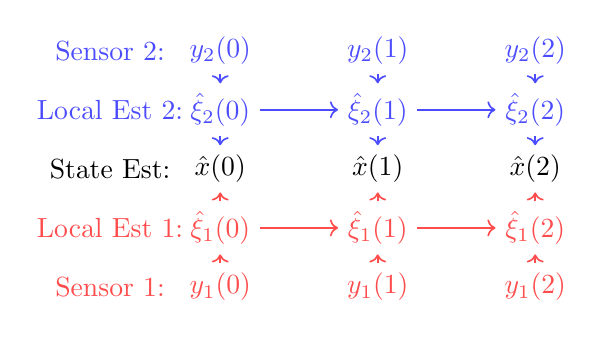
\begin{tikzpicture}[x=2cm, y=0.75cm]
      \node at (-0.7,0) {State Est:};
      \node [blue!70] at (-0.7,2) {Sensor 2:};
      \node [blue!70] at (-0.7,1) {Local Est 2:};
      \node [red!70] at (-0.7,-2) {Sensor 1:};
      \node [red!70] at (-0.7,-1) {Local Est 1:};

      \node            (x0)  at (0,0)    {$\hat x(0)$};
      \node [blue!70] (y20)  at (0,2)       {$y_2(0)$};
      \node [blue!70] (x20)  at (0,1)  {$\hat \xi_2(0)$};
      \node [red!70]  (y10)  at (0,-2)      {$y_1(0)$};
      \node [red!70]  (x10)  at (0,-1) {$\hat \xi_1(0)$};
      \draw [->,semithick,blue!70] (y20) to (x20);
      \draw [->,semithick,red!70]  (y10) to (x10);
      \draw [->,semithick,blue!70] (x20) to  (x0);
      \draw [->,semithick,red!70]  (x10) to  (x0);

      \node            (x1)  at (1,0)    {$\hat x(1)$};
      \node [blue!70] (y21)  at (1,2)       {$y_2(1)$};
      \node [blue!70] (x21)  at (1,1)  {$\hat \xi_2(1)$};
      \node [red!70]  (y11)  at (1,-2)      {$y_1(1)$};
      \node [red!70]  (x11)  at (1,-1) {$\hat \xi_1(1)$};
      \draw [->,semithick,blue!70] (y21) to (x21);
      \draw [->,semithick,red!70]  (y11) to (x11);
      \draw [->,semithick,blue!70] (x21) to  (x1);
      \draw [->,semithick,red!70]  (x11) to  (x1);

      \node            (x2)  at (2,0)    {$\hat x(2)$};
      \node [blue!70] (y22)  at (2,2)       {$y_2(2)$};
      \node [blue!70] (x22)  at (2,1)  {$\hat \xi_2(2)$};
      \node [red!70]  (y12)  at (2,-2)      {$y_1(2)$};
      \node [red!70]  (x12)  at (2,-1) {$\hat \xi_1(2)$};
      \draw [->,semithick,blue!70] (y22) to (x22);
      \draw [->,semithick,red!70]  (y12) to (x12);
      \draw [->,semithick,blue!70] (x22) to  (x2);
      \draw [->,semithick,red!70]  (x12) to  (x2);

      \draw [->,semithick,blue!70] (x20) to (x21);
      \draw [->,semithick,blue!70] (x21) to (x22);
      \draw [->,semithick,red!70] (x10) to (x11);
      \draw [->,semithick,red!70] (x11) to (x12);
    \end{tikzpicture}
  \end{center}
  \begin{itemize}
    \item It is "easy" to create a {\bf secure} or {\bf distributed} summation algorithm. 
  \end{itemize}
\end{frame}

\begin{frame}{Decomposition of Kalman filter}
  \centering
  \includegraphics[width=1.0\textwidth]{pic/decomp}
\end{frame}

\begin{frame}{Decomposition of Kalman filter}
  \begin{itemize}
    \item $(A,C)$ is observable.
      \begin{itemize}
	\item[a)] $A-KCA$ has {\color{thupurple} $n$ distinct} eigenvalues: $A-KCA=V\Lambda V^{-1}$;
	\item[b)] $A-KCA$ and $A$ {\color{thupurple}do not share} any eigenvalues.
      \end{itemize}
      \begin{theorem}

	The Kalman filter can be losslessly decomposed as a linear combination of local filters :
	\begin{align*}
	  \hat \xi_i(k+1)&=\Lambda\hat \xi_i(k)+\1_ny_i(k+1),\\
	  \hat x(k)&=\sum_{i=1}^m F_i\hat \xi_i(k),
	\end{align*}
	where $K=[K_1,\cdots,K_m]$, $F_i=V \diag(V^{-1}K_i)$, and $\hat\xi_i(k)$ is a stable estimate of $G_ix(k)$, where the span of $G_i$ is exactly the observable subspace of sensor $i$.
      \end{theorem}
  \end{itemize}
\end{frame}

%	  \begin{frame}{Decomposition of Kalman filter}
%	    \begin{itemize}
%	      \item Each sensor runs the following filter:
%		\begin{align*}
%		  \hat\xi_i(k+1)=\textcolor{thupurple}{\Lambda}\xi_i(k)+\1_n \textcolor{red}{y_i(k+1)},
%		\end{align*}
%		where $y_i(k+1)$ is not stable.
%	      \item With an equivalent transformation $z_i(k)=y_i(k+1)-\beta^T\hat\xi_i(k)$, we have
%		\begin{align*}
%		  \hat\xi_i(k+1)&=\textcolor{red}{(\Lambda+\1_n\beta^T)}\hat\xi_i(k)+\1_n\textcolor{thupurple}{z_i(k)}\\
%				&=\textcolor{red}{S}\hat\xi_i(k)+\1_n\textcolor{thupurple}{z_i(k)},
%		\end{align*}
%		where $\sum_{i=1}^n \beta_i(A-\lambda_i I)^{-1}=I$ and $S\triangleq \Lambda+\1_n\beta^T$.
%	      \item {\color{thupurple}$z_i(k)$ is stable}, i.e. $cov(z_i(k))$ is bounded.
%	      \item \textcolor{thupurple}{stable system matrix} + \textcolor{red}{unstable update} $\rightarrow$ \textcolor{red}{unstable system matrix} + \textcolor{thupurple}{stable update}.
%	    \end{itemize}
%	  \end{frame}

\section{Secure Dynamic State Estimation}


\begin{frame}{Securing the Global Estimate with LASSO}
  \begin{itemize}
    \item The Kalman estimate can be recovered as a weighted sum:
      \begin{equation*}
	  \hat x(k)=\sum_{i=1}^m F_i\hat \xi_i(k).
      \end{equation*}
    \item or as the solution of a least square problem:
      \begin{align*}
      &\mathop{\textrm{minimize}}\limits_{\hat x(k),\hat \epsilon(k)}&
      & \frac{1}{2}\hat \epsilon(k)^T \tilde W^{-1} \hat \epsilon(k)\\
      &\textrm{subject to} &
      &\hat \xi_i(k)  =  G_i\hat x(k) + \hat \epsilon_i(k),&
      \end{align*}
      where the matrix $\tilde W$ is the asymptotic covariance of $[\epsilon_1^T,\ldots ,\epsilon_n^T]$.

    \item We can secure the global estimator using LASSO:
      \begin{align*}
    &\mathop{\textrm{minimize}}\limits_{\hat x(k),\hat \epsilon(k), \hat \nu(k)}&
    & \frac{1}{2}\hat \epsilon(k)^T \tilde W^{-1} \hat \epsilon(k) + \gamma \sum_{i=1}^m \|\hat \nu_i(k)\|_1\\
    &\textrm{subject to} &
    &\hat \xi_i(k)  =  G_i\hat x(k) + \hat \epsilon_i(k)+\hat \nu_i(k).&
      \end{align*}
  \end{itemize}
\end{frame}

\begin{frame}{Efficiency and Security}
  \begin{block}{Efficiency}
    \begin{itemize}
      \item In the absence of attack, we recover the Kalman estimate if the noise is "small".
      \item Given a probability $p<1$, we can tune $\gamma$ such that we recover KF with probability $p$.
    \end{itemize}
  \end{block}
  \begin{block}{Security}
    In the presence of attack, the estimator is stable if for any $u\neq 0$ and any index set $\mathcal I$ of cardinality $c$, the following inequality hold:
    \begin{align*}
      \sum_{i\in \mathcal I} \|G_iu\|_1 < \sum_{i\in \mathcal I^c} \|G_iu\|_1. 
    \end{align*}
    If in addition, all unstable eigenvalues of $A$ matrix has geometric multiplicity of $1$, then the estimator is stable if the system is {\bf $2c$-sparse detectable}, which achieves the fundamental limit of secure state estimation.
  \end{block}
\end{frame}

\begin{frame}{Numerical Example: Inverted pendulum}
  \centering
  \begin{columns}
    \begin{column}{0.5\textwidth}
      \scalebox{0.7}{


%\tikzsetnextfilename{PIDBode}
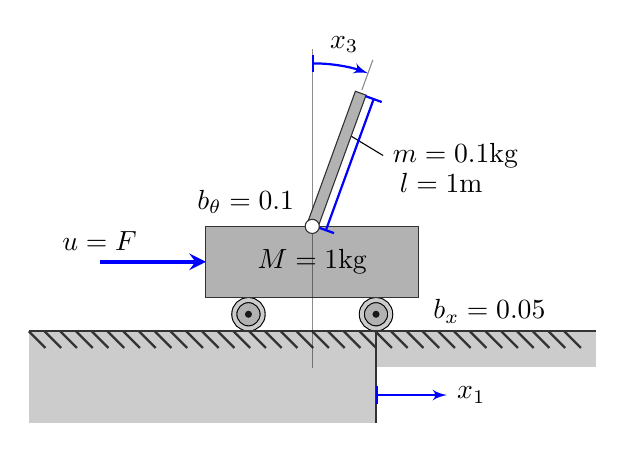
\begin{tikzpicture}[> = latex',%
	scale = 0.9]
	\tikzset{%
		interface/.style={
			% The border decoration is a path replacing decorator. 
			% For the interface style we want to draw the original path.
			% The postaction option is therefore used to ensure that the
			% border decoration is drawn *after* the original path.
			postaction={draw, decorate, decoration={border, angle=-45,
					amplitude=0.3cm, segment length=2mm}}},
		helparrow/.style={>=latex', blue, thick},
		% helparrow/.style={>=latex', draw=blue, fill=blue, very thick},
		helpline/.style={thin, black!90, opacity=0.5},
		force/.style={>=stealth, draw=blue, fill=blue, ultra thick},
	}
	\def\ground{%
		\fill [black!20] (0, 0) rectangle (49mm, -13mm);
		\fill [black!20] (49mm, 0) rectangle (80mm, -5mm);
		\draw [thick, black!80, interface] (0, 0) -- (80mm, 0);
		\draw [thick, black!80] (49mm, 0) -- +(0, -13mm);
		\draw [|->, helparrow] (49mm, -9mm) -- ++(10mm, 0) node [right] {\color{black} $x_1$ };
	}
	
	\def\cart{
		\filldraw [%thick,%
		draw = black!80,%
		fill = black!40,%
		top color = black!30,%
		bottom color = black!30,%
		% pattern=horizontal lines gray,%
		] (0,0) rectangle (30mm, 10mm);
		\node at (15mm, 5mm) {$M=1$kg};
		\draw[->, force] (-15mm, 5mm) node [above] {$u=\ensuremath{\vv{F}}$} -- (0, 5mm);
		\node at (40mm, -2mm) {$b_x = 0.05$};
	}
	
	\def\pendulum{%
		\filldraw [%thick,%
		draw = black!80,%
		% fill = black!25,%
		left color=black!30,%
		bottom color=black!30,%
		% pattern=horizontal lines gray,%
		] (-0.8mm, 0) rectangle (0.8mm, 20mm);
		\draw [|-|, helparrow] (2mm, 0mm) -- ++(0mm, 20mm);
		\node at (15mm, 12mm) {$l=1$m};
		\node at (-10mm, 0mm) {$b_\theta=0.1$}; 
	}
	
	\def\joint{%
		\filldraw [%thick,%
		draw = black!80,%
		fill = white,%
		% pattern=horizontal lines gray,%
		] (0, 0) circle (1mm);
	}
	
	\def\wheel{%
%		\fill [thin,%
%		fill = black!70,%	path fading = south
%	] (0, 0) circle (1.75mm);
%		\begin{scope}
%			\clip (0, 0) circle (1.75mm);
%			\fill [fill=black!30,] (0, -1mm) circle (2mm);
%		\end{scope}
		\fill [fill=black!30,] (0, 0mm) circle (2mm);
		\fill [fill=black!90] (0, 0) circle (0.5mm);
		\draw [thin,%
		double = black!20,%
		double distance = 0.5mm] (0, 0) circle (2mm);
	}

	\begin{scope}
		\wheel
	\end{scope}
	\begin{scope}[xshift=18mm]
		\wheel
	\end{scope}
	\begin{scope}[xshift=-31mm, yshift=-2.4mm]
		\ground
	\end{scope}
	\begin{scope}[shift = {(-6mm, 2.4mm)}]
		\cart
	\end{scope}
	\begin{scope}[shift = {(9mm, 12.4mm)}]
		\draw [helpline] (0, -20mm) -- (0, 25mm);
		\draw [helpline] (70:20.5mm) -- (70:25mm);
		\draw [|->, helparrow] (0, 23mm) 
		arc [radius=23mm, start angle=90, delta angle=-20] ;
		\node at (80:26mm) {$x_3$};
%		\draw [|->, helparrow] (0, -9mm) 
%		arc [radius=9mm, start angle=-90, delta angle=195] ;
%		\node [above right] at (50:8.5mm) {$\theta$};
		\draw [thin] (70:14mm) -- (10mm, 10mm) 
		node [right] {$m=0.1$kg};
	\end{scope}
	\begin{scope}[shift = {(9mm, 12.4mm)}, rotate=-20]
		\pendulum
	\end{scope}
	\begin{scope}[shift = {(9mm, 12.4mm)}]
		\joint
	\end{scope}
\end{tikzpicture}


%\begin{tikzpicture}[> = latex',%
%	scale = 1,%
%	text = blue]
%	\begin{scope}
%		\wheel
%	\end{scope}
%	\begin{scope}[xshift=18mm]
%		\wheel
%	\end{scope}
%	\begin{scope}[xshift=-31mm, yshift=-2.4mm]
%		\ground
%	\end{scope}
%	\begin{scope}[shift = {(-6mm, 2.4mm)}]
%		\cart
%	\end{scope}
%	\begin{scope}[shift = {(9mm, 12.4mm)}]
%		\draw [helpline] (0, -20mm) -- (0, 25mm);
%		\draw [helpline] (110:20.5mm) -- (110:25mm);
%		\draw [|->, helparrow] (0, 23mm) 
%		arc [radius=23mm, start angle=90, delta angle=20] ;
%		\node at (97:25mm) {$\theta'$};
%		\draw [|->, helparrow] (0, -9mm) 
%		arc [radius=9mm, start angle=-90, delta angle=195] ;
%		\node [above right] at (50:8.5mm) {$\theta$};
%		\draw [thin] (110:14mm) -- (-10mm, 10mm) 
%		node [left] {$m$, $I$};
%	\end{scope}
%	\begin{scope}[shift = {(9mm, 12.4mm)}, rotate=20]
%		\pendulum
%	\end{scope}
%	\begin{scope}[shift = {(9mm, 12.4mm)}]
%		\joint
%	\end{scope}
%\end{tikzpicture}}
    \end{column}
    \begin{column}{0.5\textwidth}
      $x_1$: cart position

      $x_2$: cart velocity

      $x_3$: pendulum angle

      $x_4$: pendulum angle velocity

      Linearize at $x_3=x_4=0$, 

      Sample with interval $T_s=0.02$.
    \end{column}
  \end{columns}

  \vspace{-1pt}
  {\footnotesize
    \begin{align*}
      x(k+1)=\begin{bmatrix}
	1  \hspace{-2pt}&\hspace{-2pt}   2.0\hspace{-2pt}\cdot\hspace{-2pt} 10^{-2}  \hspace{-2pt}&\hspace{-2pt}  -2.0\hspace{-2pt}\cdot\hspace{-2pt} 10^{-4}  \hspace{-2pt}&\hspace{-2pt}  1.9\hspace{-2pt}\cdot\hspace{-2pt} 10^{-5}\\
	0  \hspace{-2pt}&\hspace{-2pt}   1.0\hspace{-2pt}\cdot\hspace{-2pt} 10^{0}   \hspace{-2pt}&\hspace{-2pt} -2.0\hspace{-2pt}\cdot\hspace{-2pt} 10^{-2}  \hspace{-2pt}&\hspace{-2pt}   1.8\hspace{-2pt}\cdot\hspace{-2pt} 10^{-3}\\
	0  \hspace{-2pt}&\hspace{-2pt}   1.0\hspace{-2pt}\cdot\hspace{-2pt} 10^{-5} \hspace{-2pt}&\hspace{-2pt}   1.0\hspace{-2pt}\cdot\hspace{-2pt} 10^{0} \hspace{-2pt}&\hspace{-2pt}   2.0\hspace{-2pt}\cdot\hspace{-2pt} 10^{-2}\\
	0  \hspace{-2pt}&\hspace{-2pt}   1.0\hspace{-2pt}\cdot\hspace{-2pt} 10^{-3}\hspace{-2pt}&\hspace{-2pt}  2.1\hspace{-2pt}\cdot\hspace{-2pt} 10^{-1}  \hspace{-2pt}&\hspace{-2pt}  9.8\hspace{-2pt}\cdot\hspace{-2pt} 10^{-1}
	\end{bmatrix}x(k)+\begin{bmatrix}
	2.0\hspace{-2pt}\cdot\hspace{-2pt} 10^{-4}\\
	2.0\hspace{-2pt}\cdot\hspace{-2pt} 10^{-2}\\
	-2.0\hspace{-2pt}\cdot\hspace{-2pt} 10^{-4}\\
	-2.0\hspace{-2pt}\cdot\hspace{-2pt} 10^{-2}
      \end{bmatrix}
      u(k)+w(k).
    \end{align*}
    \begin{align*}
      y(k)=
      \begin{bmatrix}
	1\hspace{-2pt}&\hspace{-2pt} 0 \hspace{-2pt}&\hspace{-2pt}0 \hspace{-2pt}&\hspace{-2pt}0\\
	1\hspace{-2pt}&\hspace{-2pt} 0 \hspace{-2pt}&\hspace{-2pt}0 \hspace{-2pt}&\hspace{-2pt}0\\
	1\hspace{-2pt}&\hspace{-2pt} 0 \hspace{-2pt}&\hspace{-2pt}0 \hspace{-2pt}&\hspace{-2pt}0\\
	0\hspace{-2pt}&\hspace{-2pt} 0 \hspace{-2pt}&\hspace{-2pt}1 \hspace{-2pt}&\hspace{-2pt}0
      \end{bmatrix}x(k)+v(k)+a(k).
  \end{align*} }
\end{frame}
\begin{frame}{Performance without attack}
  \begin{figure}[htpb!]
    \centering
    \scalebox{0.65}{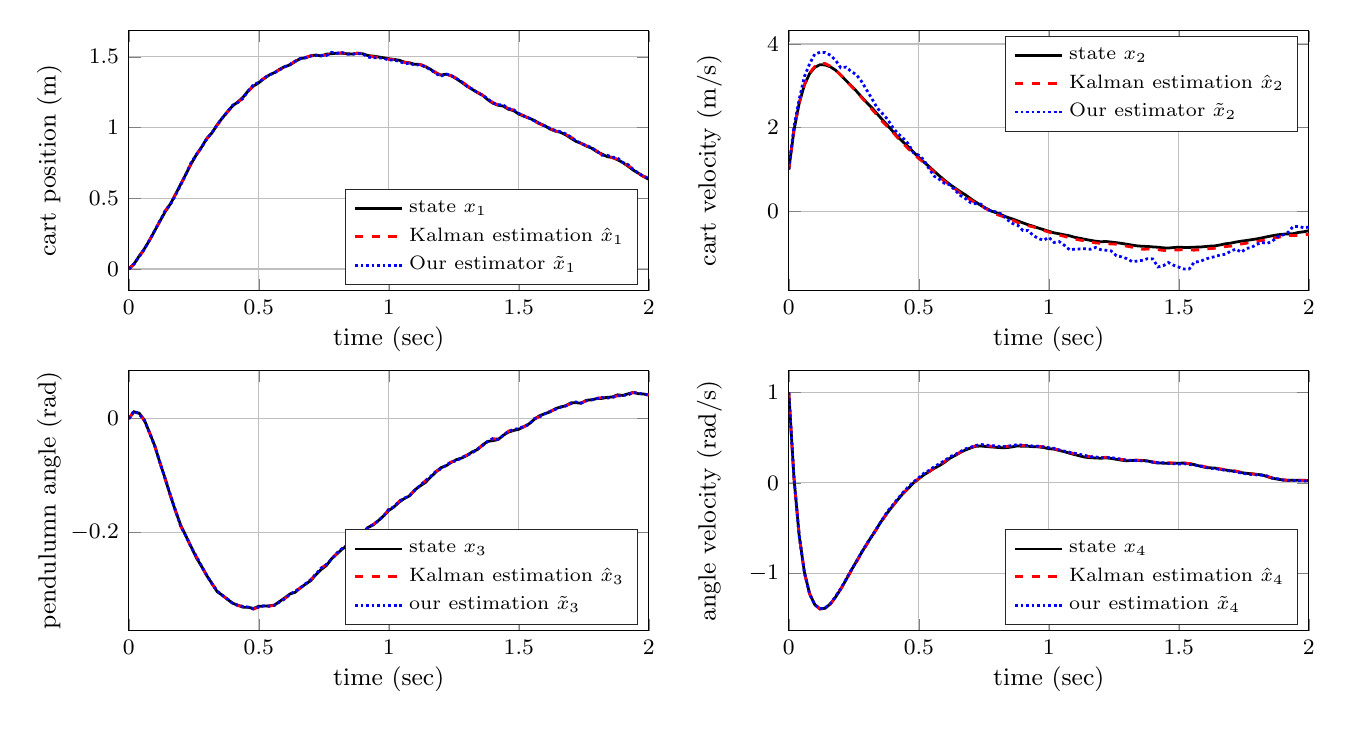
\begin{tikzpicture}
\begin{axis}
[	width=2.6in,
	height=1.3in,
	at={(0in,1.7in)},
	scale only axis,
	xmin=0,
	xmax=2.0,
	xlabel={\small time (sec)},
	ylabel={\small cart position (m)},
	x label style={at={(axis description cs:0.5,-0.1)},anchor=north},
	y label style={at={(axis description cs:-0.11,.5)},anchor=south},
	xticklabel style = {font=\footnotesize},
	yticklabel style = {font=\footnotesize},
	axis background/.style={fill=white},
	xmajorgrids,
	ymajorgrids,
	legend style={at={(0.98,0.02)}, anchor=south east, legend cell align=left, align=left, draw=white!15!black, font=\scriptsize }]
	 \addplot [color={black}, line width=1pt]
	table[row sep={\\}]
	{
 0.0  0.0  \\
0.02  0.03513048308256195  \\
0.04  0.0914419059773598  \\
0.06  0.1427778787943515  \\
0.08  0.20340397252067047  \\
0.1  0.27125016952880654  \\
0.12  0.33866874289613796  \\
0.14  0.40444843392896823  \\
0.16  0.46015949841787734  \\
0.18  0.5289069560917001  \\
0.2  0.6012564469268484  \\
0.22  0.671516604288933  \\
0.24  0.7439326698612437  \\
0.26  0.8082019623524164  \\
0.28  0.8613988630585795  \\
0.3  0.9229014124726718  \\
0.32  0.9627944492478866  \\
0.34  1.0198488236259264  \\
0.36  1.0678031171226763  \\
0.38  1.1139131874770454  \\
0.4  1.1540061381552729  \\
0.42  1.1817601868900285  \\
0.44  1.2153756793882182  \\
0.46  1.2610010644181515  \\
0.48  1.293667654117393  \\
0.5  1.3165928728936251  \\
0.52  1.3456607164297567  \\
0.54  1.3711705993370278  \\
0.56  1.3880813521098108  \\
0.58  1.4119643858187543  \\
0.6  1.4306314658383006  \\
0.62  1.4425883212114448  \\
0.64  1.4662379310448435  \\
0.66  1.4886979846322503  \\
0.68  1.4923086118898035  \\
0.7  1.5069041141339614  \\
0.72  1.5128680594921478  \\
0.74  1.505743231730095  \\
0.76  1.5189247374151202  \\
0.78  1.5218381993746002  \\
0.8  1.5255446307745213  \\
0.82  1.5253720117652096  \\
0.84  1.5217505378866258  \\
0.86  1.519753386225738  \\
0.88  1.5257526690458258  \\
0.9  1.521386537923482  \\
0.92  1.5089559694196168  \\
0.94  1.5049195077352266  \\
0.96  1.4993578292639884  \\
0.98  1.493191880058802  \\
1.0  1.4864024420058506  \\
1.02  1.4818259580594746  \\
1.04  1.475808315831528  \\
1.06  1.462990519709879  \\
1.08  1.4570631794200655  \\
1.1  1.4471759284474504  \\
1.12  1.446272982684707  \\
1.14  1.4313922548235627  \\
1.16  1.4124330091086377  \\
1.18  1.3872010233567227  \\
1.2  1.3711358431710576  \\
1.22  1.3771278026366942  \\
1.24  1.3667791681890535  \\
1.26  1.3445038037339296  \\
1.28  1.3202679649240783  \\
1.3  1.2930882108314934  \\
1.32  1.2708701152599298  \\
1.34  1.248239872310746  \\
1.36  1.2293771367777346  \\
1.38  1.1977995399651467  \\
1.4  1.172303904975972  \\
1.42  1.1579161820351642  \\
1.44  1.1518067463014627  \\
1.46  1.12924061744534  \\
1.48  1.1195894705658813  \\
1.5  1.0955432603592228  \\
1.52  1.0797265742904583  \\
1.54  1.066608150282723  \\
1.56  1.0502266993513543  \\
1.58  1.0281772752372773  \\
1.6  1.0130822665150812  \\
1.62  0.9895403519101377  \\
1.64  0.9750991121836318  \\
1.66  0.9665183092659061  \\
1.68  0.9491107003879848  \\
1.7  0.9250252075044484  \\
1.72  0.9023279997906815  \\
1.74  0.8883577172905913  \\
1.76  0.868997041684394  \\
1.78  0.8542728121099745  \\
1.8  0.8295422463647049  \\
1.82  0.812162366888937  \\
1.84  0.7943357438050268  \\
1.86  0.7883783454959857  \\
1.88  0.7721739750301243  \\
1.9  0.7527806629178648  \\
1.92  0.7271547015768657  \\
1.94  0.699425481543776  \\
1.96  0.6770173029804786  \\
1.98  0.6539652107821747  \\
2.0  0.6339162103868775  \\
	}
	;\addlegendentry{state $x_1$}
	
	\addplot [color={red},dashed, line width=1pt]
	table[row sep={\\}]
	{
 0.0  0.0  \\
0.02  0.03459224381061867  \\
0.04  0.08529450384877155  \\
0.06  0.14037092177605182  \\
0.08  0.20553954051240308  \\
0.1  0.27194944336447746  \\
0.12  0.3421140054880376  \\
0.14  0.41203750940323125  \\
0.16  0.4622193750988459  \\
0.18  0.5275770920396385  \\
0.2  0.5965866800336724  \\
0.22  0.6697110178836443  \\
0.24  0.7482230113686512  \\
0.26  0.8092656626309191  \\
0.28  0.8603169832513828  \\
0.3  0.9190552078813129  \\
0.32  0.9650153184004646  \\
0.34  1.017537438416803  \\
0.36  1.0652639550276204  \\
0.38  1.110203819001036  \\
0.4  1.1547227063481849  \\
0.42  1.1795489385299753  \\
0.44  1.2081962408148317  \\
0.46  1.2550663978277128  \\
0.48  1.29773491819716  \\
0.5  1.3202634853421826  \\
0.52  1.3485493090138312  \\
0.54  1.3730537082664092  \\
0.56  1.3887333644343987  \\
0.58  1.4096399363306875  \\
0.6  1.4291719543335981  \\
0.62  1.4458626407157713  \\
0.64  1.4681322460180737  \\
0.66  1.4857860140746912  \\
0.68  1.4965623645092951  \\
0.7  1.5064593300461164  \\
0.72  1.5105362942780847  \\
0.74  1.5102375963545158  \\
0.76  1.510715778888172  \\
0.78  1.5270954377963672  \\
0.8  1.5246804945886832  \\
0.82  1.5285375327524982  \\
0.84  1.5219032482401056  \\
0.86  1.520849497046739  \\
0.88  1.5251716736489362  \\
0.9  1.524289721395395  \\
0.92  1.505448635516613  \\
0.94  1.4999695126483625  \\
0.96  1.4960501263894108  \\
0.98  1.4934718949769015  \\
1.0  1.4818326310727334  \\
1.02  1.480707330754286  \\
1.04  1.4726414641854848  \\
1.06  1.4602017028591072  \\
1.08  1.4578204430879882  \\
1.1  1.4469453164906172  \\
1.12  1.4458062938261007  \\
1.14  1.4329313953696996  \\
1.16  1.4160364457991061  \\
1.18  1.3897188031328918  \\
1.2  1.3679973969686312  \\
1.22  1.3751905872313022  \\
1.24  1.3655727389377705  \\
1.26  1.3488207107801553  \\
1.28  1.3275020222766156  \\
1.3  1.297676742947427  \\
1.32  1.2702012536827056  \\
1.34  1.2502056805120871  \\
1.36  1.2294028774129964  \\
1.38  1.2047001213441297  \\
1.4  1.1764390180689184  \\
1.42  1.16036795764531  \\
1.44  1.155022054177548  \\
1.46  1.133504665669269  \\
1.48  1.123504538352717  \\
1.5  1.1008427846179605  \\
1.52  1.0822931182727697  \\
1.54  1.0645682653691237  \\
1.56  1.0440920436330998  \\
1.58  1.0263246901040088  \\
1.6  1.0083507822846796  \\
1.62  0.9920679329287192  \\
1.64  0.976622670428748  \\
1.66  0.965578948875552  \\
1.68  0.9523055143949263  \\
1.7  0.9325703449798766  \\
1.72  0.907991669348745  \\
1.74  0.8873053457649742  \\
1.76  0.8709858398455673  \\
1.78  0.8557650883330062  \\
1.8  0.8339912648523344  \\
1.82  0.8066085662950583  \\
1.84  0.7985872884191355  \\
1.86  0.7867861486514177  \\
1.88  0.7761000737630973  \\
1.9  0.7490347746578546  \\
1.92  0.732851128940592  \\
1.94  0.703824889092848  \\
1.96  0.6780744090491957  \\
1.98  0.6534946070984852  \\
2.0  0.6408473560775105  \\
	}
	;\addlegendentry{{ Kalman estimation $\hat{x}_1$}}
    \addplot[densely dotted, color={blue}, line width=1pt]
        table[row sep={\\}]
        {
    0.0  1.4977176879243853e-7  \\
   0.02  0.035853490924953726  \\
   0.04  0.08728505927307653  \\
   0.06  0.1402910759956027  \\
   0.08  0.20552535131997382  \\
   0.1  0.2714941202711113  \\
   0.12  0.34142780537522516  \\
   0.14  0.41073226781224864  \\
   0.16  0.4544716293659916  \\
   0.18  0.523689684730239  \\
   0.2  0.59571397823773  \\
   0.22  0.6714956021666036  \\
   0.24  0.7527759703720808  \\
   0.26  0.8099977345031584  \\
   0.28  0.8585085304808415  \\
   0.3  0.9201763916641157  \\
   0.32  0.9634570022906116  \\
   0.34  1.0194972876060886  \\
   0.36  1.0682564396376053  \\
   0.38  1.1136126645917057  \\
   0.4  1.158888312085378  \\
   0.42  1.178120027939495  \\
   0.44  1.2073589678987888  \\
   0.46  1.26043900840599  \\
   0.48  1.3032407211239458  \\
   0.5  1.3196645821997441  \\
   0.52  1.3483934150336057  \\
   0.54  1.372515904226193  \\
   0.56  1.3860504677892873  \\
   0.58  1.4085218217648232  \\
   0.6  1.4289739159288626  \\
   0.62  1.4463131599581733  \\
   0.64  1.469263537104824  \\
   0.66  1.4859403959732742  \\
   0.68  1.4946012652267906  \\
   0.7  1.5054772861342394  \\
   0.72  1.508985002964067  \\
   0.74  1.5090595106705802  \\
   0.76  1.5100025471877747  \\
   0.78  1.5316171969246877  \\
   0.8  1.5250681057932682  \\
   0.82  1.5299726074216564  \\
   0.84  1.5187812082208154  \\
   0.86  1.5179027994705732  \\
   0.88  1.5229965752350674  \\
   0.9  1.5207666604060461  \\
   0.92  1.4969719778684472  \\
   0.94  1.494447987716439  \\
   0.96  1.4922607037710425  \\
   0.98  1.4901753577011345  \\
   1.0  1.4764885137636086  \\
   1.02  1.4772125891950725  \\
   1.04  1.4682067816915458  \\
   1.06  1.4530770280512573  \\
   1.08  1.453827951153766  \\
   1.1  1.441609631566825  \\
   1.12  1.4440558602407247  \\
   1.14  1.4286081399465453  \\
   1.16  1.4105638904580435  \\
   1.18  1.3825173171614653  \\
   1.2  1.3621514478144654  \\
   1.22  1.3791831050328722  \\
   1.24  1.367315529077668  \\
   1.26  1.3476206221565943  \\
   1.28  1.3245829684293324  \\
   1.3  1.2922967385204185  \\
   1.32  1.2732201761350186  \\
   1.34  1.2489868087093448  \\
   1.36  1.2293982024530576  \\
   1.38  1.2043499531068822  \\
   1.4  1.1741781296701639  \\
   1.42  1.1611707415378525  \\
   1.44  1.1598795804587332  \\
   1.46  1.134112124666843  \\
   1.48  1.126562052033941  \\
   1.5  1.099894827177205  \\
   1.52  1.0815913921937006  \\
   1.54  1.065892705016733  \\
   1.56  1.0463019361723187  \\
   1.58  1.0286992509406694  \\
   1.6  1.0106514622486629  \\
   1.62  0.9951516048130251  \\
   1.64  0.9799038849666539  \\
   1.66  0.9700959717111278  \\
   1.68  0.9557138008265439  \\
   1.7  0.9335952475399413  \\
   1.72  0.9071514346753368  \\
   1.74  0.8872958166261384  \\
   1.76  0.8730466086745535  \\
   1.78  0.8581694338561564  \\
   1.8  0.8343792855852288  \\
   1.82  0.8049652888616172  \\
   1.84  0.8040552514089182  \\
   1.86  0.7915587983875398  \\
   1.88  0.7844327028764996  \\
   1.9  0.7527655411430587  \\
   1.92  0.7383308407971062  \\
   1.94  0.704573733557403  \\
   1.96  0.6786187118658552  \\
   1.98  0.6540139211205167  \\
   2.0  0.6447964303367395  \\
        }
        ;\addlegendentry{{ Our estimator $\tilde{x}_1$}}
        
\end{axis}

\begin{axis}
[	width=2.6in,
height=1.3in,
at={(3.3in,1.7in)},
scale only axis,
xmin=0,
xmax=2.0,
xlabel={\small time (sec)},
ylabel={\small cart velocity (m/s)},
x label style={at={(axis description cs:0.5,-0.1)},anchor=north},
y label style={at={(axis description cs:-0.11,.5)},anchor=south},
xticklabel style = {font=\footnotesize},
yticklabel style = {font=\footnotesize},
axis background/.style={fill=white},
xmajorgrids,
ymajorgrids,
legend style={at={(0.98,0.98)}, anchor=north east, legend cell align=left, align=left, draw=white!15!black, font=\scriptsize}]
\addplot [color={black}, line width=1pt]
table[row sep={\\}]
{
	   0.0  1.0  \\
	0.02  1.9334581216414537  \\
	0.04  2.5813598448326145  \\
	0.06  3.0186330460084227  \\
	0.08  3.291179056338291  \\
	0.1  3.4420274187060738  \\
	0.12  3.505817976791329  \\
	0.14  3.499891224562881  \\
	0.16  3.4541824320967547  \\
	0.18  3.3738782752424057  \\
	0.2  3.2556305585295  \\
	0.22  3.1274116627100383  \\
	0.24  3.0026901645012507  \\
	0.26  2.874184622899233  \\
	0.28  2.7341536239027664  \\
	0.3  2.599092680673387  \\
	0.32  2.474338381258081  \\
	0.34  2.3295685255856236  \\
	0.36  2.189281790708088  \\
	0.38  2.050610403342911  \\
	0.4  1.9112709141422126  \\
	0.42  1.7724690892688961  \\
	0.44  1.6556812877910012  \\
	0.46  1.5363521105995848  \\
	0.48  1.4150465701315613  \\
	0.5  1.2871220460497423  \\
	0.52  1.173898127416659  \\
	0.54  1.0669077212594953  \\
	0.56  0.9531860356888151  \\
	0.58  0.842766455685593  \\
	0.6  0.7368526011631864  \\
	0.62  0.6386885141858373  \\
	0.64  0.5522982987768248  \\
	0.66  0.4673970287861549  \\
	0.68  0.388441452040231  \\
	0.7  0.298284094139456  \\
	0.72  0.21521130663157695  \\
	0.74  0.13527244786941045  \\
	0.76  0.06775133614445589  \\
	0.78  0.0018217977639210792  \\
	0.8  -0.041362523286636844  \\
	0.82  -0.09381421061386852  \\
	0.84  -0.14407979447997937  \\
	0.86  -0.18381986538803088  \\
	0.88  -0.23073184780733264  \\
	0.9  -0.2768618767232452  \\
	0.92  -0.3221050406495692  \\
	0.94  -0.3590270204895619  \\
	0.96  -0.4031121866973199  \\
	0.98  -0.440255543871223  \\
	1.0  -0.4794506820094533  \\
	1.02  -0.5164186629794366  \\
	1.04  -0.5394774520685265  \\
	1.06  -0.5648929581179745  \\
	1.08  -0.5880335616899929  \\
	1.1  -0.6240583811993707  \\
	1.12  -0.6475946969073231  \\
	1.14  -0.6726280234431121  \\
	1.16  -0.6962591244562204  \\
	1.18  -0.716170488653756  \\
	1.2  -0.7303439029290554  \\
	1.22  -0.723794234408197  \\
	1.24  -0.7372309153786233  \\
	1.26  -0.752398594469176  \\
	1.28  -0.7689826700011977  \\
	1.3  -0.7887195432951313  \\
	1.32  -0.8098867523071835  \\
	1.34  -0.8283635747294913  \\
	1.36  -0.8385252691562912  \\
	1.38  -0.8425053705736679  \\
	1.4  -0.8530276369062237  \\
	1.42  -0.8611447646232143  \\
	1.44  -0.8755583704269705  \\
	1.46  -0.880004440081546  \\
	1.48  -0.8689920459015796  \\
	1.5  -0.8595727805783289  \\
	1.52  -0.8664261794787972  \\
	1.54  -0.8666080222698963  \\
	1.56  -0.858959104753468  \\
	1.58  -0.8582703425085555  \\
	1.6  -0.8457675726072812  \\
	1.62  -0.8351131490600251  \\
	1.64  -0.8277078898807627  \\
	1.66  -0.8050674915577795  \\
	1.68  -0.778258009757186  \\
	1.7  -0.7625851887730555  \\
	1.72  -0.7367569207114357  \\
	1.74  -0.7162352969327319  \\
	1.76  -0.7002081907735124  \\
	1.78  -0.6805254062776667  \\
	1.8  -0.6612425270314914  \\
	1.82  -0.6373058472130902  \\
	1.84  -0.610364894464108  \\
	1.86  -0.5860224964571155  \\
	1.88  -0.5644176597159203  \\
	1.9  -0.5497525352056346  \\
	1.92  -0.5436161322897733  \\
	1.94  -0.5370160070749582  \\
	1.96  -0.5071817392955478  \\
	1.98  -0.4917082598298192  \\
	2.0  -0.4666136152945374  \\
}
;\addlegendentry{state $x_2$}

\addplot [color={red},dashed, line width=1pt]
table[row sep={\\}]
{
 0.0  1.0  \\
0.02  1.947272359389003  \\
0.04  2.594445635915076  \\
0.06  3.0275370892357465  \\
0.08  3.3064047984742215  \\
0.1  3.462393973240511  \\
0.12  3.5337552017316733  \\
0.14  3.5316267806993924  \\
0.16  3.470940986138043  \\
0.18  3.376126341013576  \\
0.2  3.2566259086770186  \\
0.22  3.120943910267192  \\
0.24  2.994733431504582  \\
0.26  2.8615793698700442  \\
0.28  2.7190991877286375  \\
0.3  2.5871944838338887  \\
0.32  2.4357929803750835  \\
0.34  2.297296006782219  \\
0.36  2.146799297184839  \\
0.38  2.018946597493442  \\
0.4  1.889014652512622  \\
0.42  1.7487315098372516  \\
0.44  1.624824088563198  \\
0.46  1.4897200993389361  \\
0.48  1.3810698328950473  \\
0.5  1.2596631340531221  \\
0.52  1.1634939872696184  \\
0.54  1.0480627830829743  \\
0.56  0.9308302914400389  \\
0.58  0.8123785236046864  \\
0.6  0.7148330468660997  \\
0.62  0.6265455625597441  \\
0.64  0.5331502434450455  \\
0.66  0.43205816222084126  \\
0.68  0.3483303867886185  \\
0.7  0.2658684830316831  \\
0.72  0.1986892314490598  \\
0.74  0.12940453547456832  \\
0.76  0.057090111696830426  \\
0.78  -0.022323517297730522  \\
0.8  -0.07855954509213436  \\
0.82  -0.1196590633380139  \\
0.84  -0.16482030375100798  \\
0.86  -0.21334051972282897  \\
0.88  -0.26764929753246003  \\
0.9  -0.3085925202001949  \\
0.92  -0.34729926263317723  \\
0.94  -0.37389141047737684  \\
0.96  -0.4186172810225557  \\
0.98  -0.4604016560194364  \\
1.0  -0.49774276614583723  \\
1.02  -0.5415613192539162  \\
1.04  -0.5732363853566289  \\
1.06  -0.6009216622984934  \\
1.08  -0.6361620967828028  \\
1.1  -0.6662684185318611  \\
1.12  -0.6910234803017076  \\
1.14  -0.7091492500091724  \\
1.16  -0.7326867589147015  \\
1.18  -0.7583372537059867  \\
1.2  -0.7678701553484749  \\
1.22  -0.775291203531666  \\
1.24  -0.7826361711427366  \\
1.26  -0.7891963194264477  \\
1.28  -0.8137146002990012  \\
1.3  -0.8366439913742113  \\
1.32  -0.8590459273741499  \\
1.34  -0.8777808029848111  \\
1.36  -0.9088564448755428  \\
1.38  -0.9052762284220978  \\
1.4  -0.9103017076540781  \\
1.42  -0.9217620312291152  \\
1.44  -0.9360252496793352  \\
1.46  -0.9439912115605257  \\
1.48  -0.9257262139038105  \\
1.5  -0.9248197561970852  \\
1.52  -0.9208562202142578  \\
1.54  -0.9280099457265346  \\
1.56  -0.9307959004598831  \\
1.58  -0.9226143412383395  \\
1.6  -0.9040398340982976  \\
1.62  -0.8937141414658287  \\
1.64  -0.8857428368393998  \\
1.66  -0.866305242987084  \\
1.68  -0.8441684653507048  \\
1.7  -0.8353086527257382  \\
1.72  -0.8050702996023907  \\
1.74  -0.7845056910274278  \\
1.76  -0.7650158652157595  \\
1.78  -0.7376887920799782  \\
1.8  -0.723084297668014  \\
1.82  -0.6992720095891855  \\
1.84  -0.677183773374071  \\
1.86  -0.6432509338919762  \\
1.88  -0.6298213424768249  \\
1.9  -0.5970448968271864  \\
1.92  -0.5853791165420197  \\
1.94  -0.5788058486799379  \\
1.96  -0.5782348686628517  \\
1.98  -0.5671551428159235  \\
2.0  -0.551581774220117  \\
}
;\addlegendentry{{ Kalman estimation $\hat{x}_2$}}
\addplot[densely dotted, color={blue}, line width=1pt]
table[row sep={\\}]
{
 0.0  0.9999999921251895  \\
0.02  2.0212895754401674  \\
0.04  2.6756392857258184  \\
0.06  3.221956367906082  \\
0.08  3.524459948415112  \\
0.1  3.7597636021985625  \\
0.12  3.801231238982991  \\
0.14  3.799637195005116  \\
0.16  3.7327542013131265  \\
0.18  3.6111856404678333  \\
0.2  3.430534859904597  \\
0.22  3.4485602236994395  \\
0.24  3.3444533813093464  \\
0.26  3.2665237848301816  \\
0.28  3.1042853013055063  \\
0.3  2.8967222342877976  \\
0.32  2.6907577163441476  \\
0.34  2.470727224887547  \\
0.36  2.33691826338607  \\
0.38  2.200387456547136  \\
0.4  2.0020638149880137  \\
0.42  1.8570627601031489  \\
0.44  1.747672024063133  \\
0.46  1.611155911903882  \\
0.48  1.3963895051585353  \\
0.5  1.3408628051804476  \\
0.52  1.2247463441132191  \\
0.54  1.010654566111314  \\
0.56  0.8344555369735892  \\
0.58  0.7584015792726887  \\
0.6  0.6632429865275014  \\
0.62  0.6293946727583775  \\
0.64  0.4985199207634023  \\
0.66  0.37640264139319624  \\
0.68  0.3011719349763173  \\
0.7  0.20268409454240105  \\
0.72  0.17876010231844372  \\
0.74  0.16927357874176333  \\
0.76  0.04338529646943603  \\
0.78  0.002109695471169712  \\
0.8  -0.01550391409818583  \\
0.82  -0.0747172626157792  \\
0.84  -0.20114517757971595  \\
0.86  -0.29154879522700883  \\
0.88  -0.3342275025568856  \\
0.9  -0.46051997938139294  \\
0.92  -0.4592290442747301  \\
0.94  -0.5784388075160722  \\
0.96  -0.6525450159385416  \\
0.98  -0.695320153788558  \\
1.0  -0.6240888206867699  \\
1.02  -0.7463217729066517  \\
1.04  -0.726975101951553  \\
1.06  -0.8138167061427473  \\
1.08  -0.9235454222917523  \\
1.1  -0.9069665295941886  \\
1.12  -0.9006953548896325  \\
1.14  -0.8974900363513572  \\
1.16  -0.9094084162227737  \\
1.18  -0.8664730452439139  \\
1.2  -0.9202891565839497  \\
1.22  -0.9328018978926498  \\
1.24  -0.9508543283041255  \\
1.26  -1.0646735023491174  \\
1.28  -1.0912248536913043  \\
1.3  -1.1331402926510883  \\
1.32  -1.203643871217519  \\
1.34  -1.1922974521406433  \\
1.36  -1.1738986207825004  \\
1.38  -1.1350262927165347  \\
1.4  -1.1414974965228946  \\
1.42  -1.331862785682863  \\
1.44  -1.3060932513394654  \\
1.46  -1.2275118049260128  \\
1.48  -1.2914442441963048  \\
1.5  -1.3372485123883435  \\
1.52  -1.3820301256548315  \\
1.54  -1.3821000075562804  \\
1.56  -1.2137564286546132  \\
1.58  -1.207557673691415  \\
1.6  -1.1516263695735407  \\
1.62  -1.1129690587856955  \\
1.64  -1.0850379975163027  \\
1.66  -1.045131304276628  \\
1.68  -1.0292639388423739  \\
1.7  -0.9523308895320762  \\
1.72  -0.905240368310937  \\
1.74  -0.9804802293648478  \\
1.76  -0.8910154468115234  \\
1.78  -0.8648663571953334  \\
1.8  -0.7900802207875451  \\
1.82  -0.7486111807501488  \\
1.84  -0.769284934870073  \\
1.86  -0.7162288714699678  \\
1.88  -0.6108822217212676  \\
1.9  -0.5685703272065101  \\
1.92  -0.5058158657185248  \\
1.94  -0.3633224811381064  \\
1.96  -0.3634413413786554  \\
1.98  -0.393417228111549  \\
2.0  -0.38005238786555934  \\
}
;\addlegendentry{{ Our estimator $\tilde{x}_2$}}

\end{axis}

  	\begin{axis}
	[	width=2.6in,
	height=1.3in,
	at={(0in,0in)},
	scale only axis,
	xmin=0,
	xmax=2.0,
%	ymin=-4,
%	ymax=2,
	xlabel={\small time (sec)},
	ylabel={\small pendulumn angle (rad)},
	x label style={at={(axis description cs:0.5,-0.1)},anchor=north},
	y label style={at={(axis description cs:-0.11,.5)},anchor=south},
	xticklabel style = {font=\footnotesize},
	yticklabel style = {font=\footnotesize},
	axis background/.style={fill=white},
	xmajorgrids,
	ymajorgrids,
	legend style={at={(0.98,0.02)}, anchor=south east, legend cell align=left, align=left, draw=white!15!black, font=\scriptsize}]
	\addplot [color={black}, line width=1pt]
	table[row sep={\\}]
	{
	0.0  0.0  \\
	0.02  0.012291107212995766  \\
	0.04  0.009755897813268646  \\
	0.06  -0.0021158879924274895  \\
	0.08  -0.0247027096213208  \\
	0.1  -0.04772264515761605  \\
	0.12  -0.07760140828511264  \\
	0.14  -0.10540107095412833  \\
	0.16  -0.13522977096567482  \\
	0.18  -0.1625910350853779  \\
	0.2  -0.18762454463647446  \\
	0.22  -0.20648175697703935  \\
	0.24  -0.2253718219740834  \\
	0.26  -0.2446837803311821  \\
	0.28  -0.2598043838864768  \\
	0.3  -0.27605718927768963  \\
	0.32  -0.29005282855504183  \\
	0.34  -0.3042957897577329  \\
	0.36  -0.31049253276580696  \\
	0.38  -0.3180784063475375  \\
	0.4  -0.3246605763946356  \\
	0.42  -0.3281158539923102  \\
	0.44  -0.3316915860721911  \\
	0.46  -0.331794893198938  \\
	0.48  -0.33385309324954493  \\
	0.5  -0.3298748808806763  \\
	0.52  -0.32962332567317526  \\
	0.54  -0.32935520726148154  \\
	0.56  -0.3278096251813507  \\
	0.58  -0.32156766834611766  \\
	0.6  -0.31514570998488606  \\
	0.62  -0.3082586040066044  \\
	0.64  -0.30531014110059096  \\
	0.66  -0.2974893495725164  \\
	0.68  -0.2909982672931626  \\
	0.7  -0.28476233098070064  \\
	0.72  -0.2741691441756372  \\
	0.74  -0.26514320719682183  \\
	0.76  -0.25834616090694207  \\
	0.78  -0.2463839079177759  \\
	0.8  -0.23800597979646262  \\
	0.82  -0.2297059475101298  \\
	0.84  -0.22320522465660433  \\
	0.86  -0.21473029965939316  \\
	0.88  -0.2078124562987345  \\
	0.9  -0.20054438831726454  \\
	0.92  -0.191255406523477  \\
	0.94  -0.18694955107462255  \\
	0.96  -0.17918753992578848  \\
	0.98  -0.1709426605116633  \\
	1.0  -0.1613919061973941  \\
	1.02  -0.15508350580114946  \\
	1.04  -0.14671305238418206  \\
	1.06  -0.1403268225084615  \\
	1.08  -0.13574733780874354  \\
	1.1  -0.12525543807074938  \\
	1.12  -0.11830891826074295  \\
	1.14  -0.11245711089028443  \\
	1.16  -0.10307527657908676  \\
	1.18  -0.09427290168258842  \\
	1.2  -0.08624311487904997  \\
	1.22  -0.08281286220423259  \\
	1.24  -0.07694032858147544  \\
	1.26  -0.07202084211561871  \\
	1.28  -0.06915277041228256  \\
	1.3  -0.06482535296933563  \\
	1.32  -0.0585286985478911  \\
	1.34  -0.0544178260128904  \\
	1.36  -0.04631622791370163  \\
	1.38  -0.039964573256803776  \\
	1.4  -0.03847838945946058  \\
	1.42  -0.03672894464324935  \\
	1.44  -0.029174405131490357  \\
	1.46  -0.02359523707621013  \\
	1.48  -0.020619335181098767  \\
	1.5  -0.018521871195534556  \\
	1.52  -0.014018688360862593  \\
	1.54  -0.00887576952604927  \\
	1.56  -0.0009549249582036146  \\
	1.58  0.005369382629282453  \\
	1.6  0.008923746760306408  \\
	1.62  0.012014243079846536  \\
	1.64  0.017493783523120362  \\
	1.66  0.02063669578966442  \\
	1.68  0.022777301401473927  \\
	1.7  0.02792901936340122  \\
	1.72  0.0283241284450547  \\
	1.74  0.027254422457167155  \\
	1.76  0.032589984297573586  \\
	1.78  0.03338585890332495  \\
	1.8  0.035379761925010626  \\
	1.82  0.035895798593158466  \\
	1.84  0.0377253385620041  \\
	1.86  0.0383662690861781  \\
	1.88  0.04210618064021919  \\
	1.9  0.041098254254943775  \\
	1.92  0.04377317376047081  \\
	1.94  0.04648024578966923  \\
	1.96  0.04418348421073788  \\
	1.98  0.043582409046281606  \\
	2.0  0.04168602319521932  \\
	}
	;\addlegendentry{state $x_3$}
	\addplot [color={red},dashed, line width=1pt]
	table[row sep={\\}]
	{
	 0.0  0.0  \\
	0.02  0.013426852424592635  \\
	0.04  0.00843301396563128  \\
	0.06  -0.0032719716704107363  \\
	0.08  -0.02481652590182395  \\
	0.1  -0.0481640290053725  \\
	0.12  -0.0773260791503746  \\
	0.14  -0.1058336782375687  \\
	0.16  -0.13437583604937386  \\
	0.18  -0.16212078795551588  \\
	0.2  -0.18936680035330689  \\
	0.22  -0.20682682816877246  \\
	0.24  -0.22624739266974847  \\
	0.26  -0.24255240711015966  \\
	0.28  -0.25938100915865997  \\
	0.3  -0.27582223696323216  \\
	0.32  -0.29017509895378113  \\
	0.34  -0.30312551898597867  \\
	0.36  -0.3108404318615062  \\
	0.38  -0.3175096992310906  \\
	0.4  -0.32477739971223507  \\
	0.42  -0.32872249274395  \\
	0.44  -0.33018903736083494  \\
	0.46  -0.33157421359120864  \\
	0.48  -0.3347682789953573  \\
	0.5  -0.3312864817244998  \\
	0.52  -0.3291627726596654  \\
	0.54  -0.3297666385420164  \\
	0.56  -0.3282382129572867  \\
	0.58  -0.32238470924044726  \\
	0.6  -0.31672569552127106  \\
	0.62  -0.3085504873331749  \\
	0.64  -0.30358250382869933  \\
	0.66  -0.29773744780767014  \\
	0.68  -0.29016275624136845  \\
	0.7  -0.28324232741969124  \\
	0.72  -0.2732071282504288  \\
	0.74  -0.26281750327886394  \\
	0.76  -0.2564093284426296  \\
	0.78  -0.24688582045630497  \\
	0.8  -0.23677699922420448  \\
	0.82  -0.22836242552414882  \\
	0.84  -0.22245410156213347  \\
	0.86  -0.21530514692305724  \\
	0.88  -0.20682501773654127  \\
	0.9  -0.20132726494700445  \\
	0.92  -0.19133634121209478  \\
	0.94  -0.1860795054846685  \\
	0.96  -0.17923265589551396  \\
	0.98  -0.17123226535783656  \\
	1.0  -0.15947304935805745  \\
	1.02  -0.1548388172456593  \\
	1.04  -0.14520227739515446  \\
	1.06  -0.13967063081873776  \\
	1.08  -0.13497786067807926  \\
	1.1  -0.12577412934247395  \\
	1.12  -0.1175337223799782  \\
	1.14  -0.10944005723868216  \\
	1.16  -0.10203913130146214  \\
	1.18  -0.09308715477437135  \\
	1.2  -0.08794796965792803  \\
	1.22  -0.08185246218716763  \\
	1.24  -0.07600601687938979  \\
	1.26  -0.07381608821932717  \\
	1.28  -0.06864813536384877  \\
	1.3  -0.06395460212857695  \\
	1.32  -0.0602261386722721  \\
	1.34  -0.05382440640690687  \\
	1.36  -0.04712363867652214  \\
	1.38  -0.04002379686199878  \\
	1.4  -0.03497080113403436  \\
	1.42  -0.036111152278679635  \\
	1.44  -0.029620305752766234  \\
	1.46  -0.021773164700165097  \\
	1.48  -0.019294421438656367  \\
	1.5  -0.016478689404025585  \\
	1.52  -0.013809213558272245  \\
	1.54  -0.009727493539955652  \\
	1.56  0.00010697132410502795  \\
	1.58  0.003604031000592948  \\
	1.6  0.008688099632814618  \\
	1.62  0.012944729342028295  \\
	1.64  0.016592536427066158  \\
	1.66  0.020277043802924465  \\
	1.68  0.02257961530726481  \\
	1.7  0.026839618915516762  \\
	1.72  0.029657998521030172  \\
	1.74  0.027805946665924633  \\
	1.76  0.03180101991605573  \\
	1.78  0.033066821117509665  \\
	1.8  0.035885805832444086  \\
	1.82  0.03732698332095191  \\
	1.84  0.03641690235064062  \\
	1.86  0.037608010230084615  \\
	1.88  0.04046959465662314  \\
	1.9  0.04083718635296667  \\
	1.92  0.042140952368440815  \\
	1.94  0.046116066215212054  \\
	1.96  0.04496044143824164  \\
	1.98  0.042846010266078184  \\
	2.0  0.04215378271487344  \\
	}
	;\addlegendentry{{ Kalman estimation $\hat{x}_3$}}
	\addplot[densely dotted, color={blue}, line width=1pt]
	table[row sep={\\}]
	{
	  0.0  3.1433028608416316e-11  \\
	0.02  0.01344847021277637  \\
	0.04  0.008456418975972609  \\
	0.06  -0.003219574862069982  \\
	0.08  -0.02475805266926738  \\
	0.1  -0.048084890121452485  \\
	0.12  -0.07725623252920924  \\
	0.14  -0.10576373127871824  \\
	0.16  -0.1343109389730368  \\
	0.18  -0.16206335020175422  \\
	0.2  -0.1893260123921801  \\
	0.22  -0.20674474366208784  \\
	0.24  -0.22615857471885029  \\
	0.26  -0.24244984963046978  \\
	0.28  -0.2592849482472964  \\
	0.3  -0.27574565258076134  \\
	0.32  -0.29011468126158285  \\
	0.34  -0.3030849181196164  \\
	0.36  -0.31079415153767914  \\
	0.38  -0.31746475450630307  \\
	0.4  -0.32475059932585915  \\
	0.42  -0.3286979958750598  \\
	0.44  -0.3301566350657236  \\
	0.46  -0.3315454057362295  \\
	0.48  -0.33476539666787736  \\
	0.5  -0.33126459223915605  \\
	0.52  -0.3291446171754128  \\
	0.54  -0.32977682333152664  \\
	0.56  -0.3282644310786887  \\
	0.58  -0.32239992793632893  \\
	0.6  -0.3167376923759136  \\
	0.62  -0.3085475743064995  \\
	0.64  -0.30359190886766  \\
	0.66  -0.29775518117534255  \\
	0.68  -0.2901767867638945  \\
	0.7  -0.2832625348316812  \\
	0.72  -0.2732108435292309  \\
	0.74  -0.26280663960011597  \\
	0.76  -0.2564159355046562  \\
	0.78  -0.24688204211903556  \\
	0.8  -0.23676259103857464  \\
	0.82  -0.22835230844078408  \\
	0.84  -0.22246562892342184  \\
	0.86  -0.21532691142003657  \\
	0.88  -0.2068442861454246  \\
	0.9  -0.20136824017592664  \\
	0.92  -0.19136447635253848  \\
	0.94  -0.1861313446823315  \\
	0.96  -0.17929319817646316  \\
	0.98  -0.1712913427238095  \\
	1.0  -0.15950353420499566  \\
	1.02  -0.15489450584642925  \\
	1.04  -0.14524273291189224  \\
	1.06  -0.13972735953720475  \\
	1.08  -0.13505461765357452  \\
	1.1  -0.12583533518582937  \\
	1.12  -0.11758925372920472  \\
	1.14  -0.10948757785994269  \\
	1.16  -0.10208415445996129  \\
	1.18  -0.09311647703886469  \\
	1.2  -0.08798920559108425  \\
	1.22  -0.08189633429516247  \\
	1.24  -0.07605045258975703  \\
	1.26  -0.07388888332934941  \\
	1.28  -0.06872358366327118  \\
	1.3  -0.06403512588379763  \\
	1.32  -0.06031880849722568  \\
	1.34  -0.05390843262445146  \\
	1.36  -0.047195908591125865  \\
	1.38  -0.040084203489465196  \\
	1.4  -0.03503401262632256  \\
	1.42  -0.036220695262529044  \\
	1.44  -0.029718190884273927  \\
	1.46  -0.021848754400959458  \\
	1.48  -0.01939066854636683  \\
	1.5  -0.0165878607075766  \\
	1.52  -0.01393033314624452  \\
	1.54  -0.00984796249146883  \\
	1.56  3.2439964015529796e-5  \\
	1.58  0.003528261632672118  \\
	1.6  0.00862371058623918  \\
	1.62  0.012887565405679638  \\
	1.64  0.016540197860918194  \\
	1.66  0.020229548981544734  \\
	1.68  0.022530692928118046  \\
	1.7  0.026807904118887373  \\
	1.72  0.029632732673344667  \\
	1.74  0.027753413760428246  \\
	1.76  0.03176884410287142  \\
	1.78  0.03303614023475411  \\
	1.8  0.035869861526218454  \\
	1.82  0.037316297307355514  \\
	1.84  0.036393231851024214  \\
	1.86  0.037593384983039296  \\
	1.88  0.04047659192861037  \\
	1.9  0.04084873814081459  \\
	1.92  0.04216512575394451  \\
	1.94  0.04617317081672683  \\
	1.96  0.04501482701743717  \\
	1.98  0.04288794903185354  \\
	2.0  0.04219731519953074  \\
	}
;\addlegendentry{{our estimation $\tilde{x}_3$}}


\end{axis}

\begin{axis}
[	width=2.6in,
height=1.3in,
at={(3.3in,0in)},
scale only axis,
xmin=0,
xmax=2.0,
%ymin=-4,
%ymax=2,
xlabel={\small time (sec)},
ylabel={\small angle velocity (rad/s)},
x label style={at={(axis description cs:0.5,-0.1)},anchor=north},
y label style={at={(axis description cs:-0.11,.5)},anchor=south},
xticklabel style = {font=\footnotesize},
yticklabel style = {font=\footnotesize},
axis background/.style={fill=white},
xmajorgrids,
ymajorgrids,
legend style={at={(0.98,0.02)}, anchor=south east, legend cell align=left, align=left, draw=white!15!black, font=\scriptsize}]
\addplot [color={black}, line width=1pt]
table[row sep={\\}]
{
  0.0  1.0  \\
0.02  0.05313305390126177  \\
0.04  -0.5807597079886778  \\
0.06  -0.9849649892184913  \\
0.08  -1.2236616544745775  \\
0.1  -1.3448708265564777  \\
0.12  -1.3911973425235322  \\
0.14  -1.3847017109780744  \\
0.16  -1.3360588370385862  \\
0.18  -1.2612956960549269  \\
0.2  -1.1712121233640451  \\
0.22  -1.071999578445813  \\
0.24  -0.9674797110228057  \\
0.26  -0.8680549183886634  \\
0.28  -0.7699884280336178  \\
0.3  -0.6746842796248621  \\
0.32  -0.586875654761506  \\
0.34  -0.4959299174041296  \\
0.36  -0.40597661697079446  \\
0.38  -0.32771095994654365  \\
0.4  -0.253961547290701  \\
0.42  -0.18263871652089975  \\
0.44  -0.11573407741218594  \\
0.46  -0.05911515161120641  \\
0.48  0.0009801138197992887  \\
0.5  0.04463813200237973  \\
0.52  0.09038368590143643  \\
0.54  0.12381466371390598  \\
0.56  0.16193471899976158  \\
0.58  0.19217803962499197  \\
0.6  0.2284585486584002  \\
0.62  0.27315223526991256  \\
0.64  0.3029744279918313  \\
0.66  0.3360381761463694  \\
0.68  0.36405311581028843  \\
0.7  0.3862145241118462  \\
0.72  0.4052381391063923  \\
0.74  0.40659407112164414  \\
0.76  0.4016463115722345  \\
0.78  0.39680426743202124  \\
0.8  0.3921338510569967  \\
0.82  0.3884591608505884  \\
0.84  0.3897778445333768  \\
0.86  0.3978434385510643  \\
0.88  0.40888248291393214  \\
0.9  0.40349125898703586  \\
0.92  0.4043181979298124  \\
0.94  0.4001713487291486  \\
0.96  0.397537790317619  \\
0.98  0.3906342747298136  \\
1.0  0.377882856254513  \\
1.02  0.3727858562415341  \\
1.04  0.3579748382263377  \\
1.06  0.34457979003538486  \\
1.08  0.3274365776280705  \\
1.1  0.31223393396172927  \\
1.12  0.2972605478138003  \\
1.14  0.28374482940224277  \\
1.16  0.27808313315371463  \\
1.18  0.2752540519763583  \\
1.2  0.27226461109496636  \\
1.22  0.27696110635321103  \\
1.24  0.26990768271144283  \\
1.26  0.26054532527838425  \\
1.28  0.2504740216554849  \\
1.3  0.24312004848395827  \\
1.32  0.24828658502523776  \\
1.34  0.2471687742404289  \\
1.36  0.2483512476352048  \\
1.38  0.2421106054905815  \\
1.4  0.2281155213543221  \\
1.42  0.2192043397969218  \\
1.44  0.21813440821530206  \\
1.46  0.215847499113375  \\
1.48  0.21810640903792972  \\
1.5  0.21793606071633792  \\
1.52  0.21839791991053367  \\
1.54  0.21094224607272868  \\
1.56  0.20175648284456538  \\
1.58  0.18577552098976302  \\
1.6  0.17234252915874954  \\
1.62  0.1667589628096436  \\
1.64  0.16336600936391402  \\
1.66  0.15026901018454916  \\
1.68  0.1427360828668787  \\
1.7  0.13367410170858618  \\
1.72  0.12734499958354706  \\
1.74  0.11405351681196844  \\
1.76  0.10587244286568445  \\
1.78  0.10156266429081387  \\
1.8  0.0936679758808678  \\
1.82  0.08822122445956102  \\
1.84  0.07018133601995245  \\
1.86  0.05094537909202273  \\
1.88  0.04130087142500513  \\
1.9  0.032313361980953  \\
1.92  0.02866897811479254  \\
1.94  0.030018199155337016  \\
1.96  0.029179914657290675  \\
1.98  0.029178093401201616  \\
2.0  0.02640041419686011  \\
}
;\addlegendentry{state $x_4$}
\addplot [color={red},dashed, line width=1pt]
table[row sep={\\}]
{
0.0  1.0  \\
0.02  0.05196229099537668  \\
0.04  -0.5824313535988286  \\
0.06  -0.9891377715191895  \\
0.08  -1.225040556372666  \\
0.1  -1.3474376677420603  \\
0.12  -1.3927650448471267  \\
0.14  -1.3853875418228592  \\
0.16  -1.3385535189542455  \\
0.18  -1.2616908106226903  \\
0.2  -1.1733481356619362  \\
0.22  -1.0733971982561636  \\
0.24  -0.9709048883726853  \\
0.26  -0.8734509930998627  \\
0.28  -0.7737477786715035  \\
0.3  -0.6814462079764667  \\
0.32  -0.5930068323706987  \\
0.34  -0.5011111690344067  \\
0.36  -0.4117486708366517  \\
0.38  -0.32787217975647187  \\
0.4  -0.25500615240975977  \\
0.42  -0.18223637558459482  \\
0.44  -0.1136859116043202  \\
0.46  -0.05435490540626656  \\
0.48  0.001052155333388885  \\
0.5  0.047862836014496535  \\
0.52  0.09307612385402939  \\
0.54  0.12661541422593295  \\
0.56  0.16673898540858903  \\
0.58  0.20040364092746082  \\
0.6  0.2378257684031066  \\
0.62  0.28092995786664526  \\
0.64  0.30722850104675375  \\
0.66  0.33988761950874746  \\
0.68  0.3717014698259486  \\
0.7  0.39114473419457757  \\
0.72  0.41074056965705785  \\
0.74  0.4157082365437478  \\
0.76  0.4107206907578836  \\
0.78  0.40479797621004415  \\
0.8  0.4002479612239634  \\
0.82  0.39670525295180864  \\
0.84  0.402980720989716  \\
0.86  0.40966660580558506  \\
0.88  0.41939855229643713  \\
0.9  0.4136774603389678  \\
0.92  0.41337706589827294  \\
0.94  0.4076360923733703  \\
0.96  0.40419133912255345  \\
0.98  0.39738214224816115  \\
1.0  0.38613613596819135  \\
1.02  0.37863833492291044  \\
1.04  0.3613171630485197  \\
1.06  0.34817084130208276  \\
1.08  0.3337665386001098  \\
1.1  0.322513876054837  \\
1.12  0.30951293238535926  \\
1.14  0.29822140789925367  \\
1.16  0.2887209415996951  \\
1.18  0.2855447198327156  \\
1.2  0.2792019100681843  \\
1.22  0.28259480121327957  \\
1.24  0.27674766540821855  \\
1.26  0.2679337895584435  \\
1.28  0.25957147095312993  \\
1.3  0.2512852868921737  \\
1.32  0.25335034594023265  \\
1.34  0.2517049563980485  \\
1.36  0.24854241554762116  \\
1.38  0.2437570887642059  \\
1.4  0.232081337423728  \\
1.42  0.2246763936573522  \\
1.44  0.22593853025256636  \\
1.46  0.22180580292165525  \\
1.48  0.2201777881736648  \\
1.5  0.21772174841998373  \\
1.52  0.22039359761167476  \\
1.54  0.21451665272588324  \\
1.56  0.20671496543671092  \\
1.58  0.19237907013470915  \\
1.6  0.17849341727408496  \\
1.62  0.1693669711801831  \\
1.64  0.1654694365161853  \\
1.66  0.15476608715270937  \\
1.68  0.14644491458503275  \\
1.7  0.1380087312073818  \\
1.72  0.12999696162763208  \\
1.74  0.11642996712779241  \\
1.76  0.10651977489569771  \\
1.78  0.09914327961373791  \\
1.8  0.09326070775598083  \\
1.82  0.08760116773835838  \\
1.84  0.07441328030636729  \\
1.86  0.0534154762075595  \\
1.88  0.04537417203289343  \\
1.9  0.03311477519912949  \\
1.92  0.029386264188961075  \\
1.94  0.031449452742925314  \\
1.96  0.028203792066178256  \\
1.98  0.026902194874244584  \\
2.0  0.023968301890876745  \\
}
;\addlegendentry{{ Kalman estimation $\hat{x}_4$}}
\addplot[densely dotted, color={blue}, line width=1pt]
table[row sep={\\}]
{
   0.0  0.9999999995931783  \\
0.02  0.053256438469400355  \\
0.04  -0.5810558367590097  \\
0.06  -0.9888797959421549  \\
0.08  -1.223881505907738  \\
0.1  -1.3453082018539748  \\
0.12  -1.3891303460776288  \\
0.14  -1.379673068887711  \\
0.16  -1.3337025957314825  \\
0.18  -1.253342000372752  \\
0.2  -1.165825320019194  \\
0.22  -1.0647406851480974  \\
0.24  -0.962864368017885  \\
0.26  -0.8669013996514804  \\
0.28  -0.7648147896002787  \\
0.3  -0.6716102653407486  \\
0.32  -0.5837308230993299  \\
0.34  -0.49443467840184724  \\
0.36  -0.40249690841846597  \\
0.38  -0.3131891235819798  \\
0.4  -0.2447579085019484  \\
0.42  -0.17249116699733316  \\
0.44  -0.1030719454933759  \\
0.46  -0.04285668755265462  \\
0.48  0.0114903655938736  \\
0.5  0.058227653678667265  \\
0.52  0.10717166963032067  \\
0.54  0.1384072775498972  \\
0.56  0.18001465974339406  \\
0.58  0.2133703433896741  \\
0.6  0.2465157229825645  \\
0.62  0.28971937610144716  \\
0.64  0.3129481166649311  \\
0.66  0.3450497044394353  \\
0.68  0.37686103961345435  \\
0.7  0.3936878232730471  \\
0.72  0.4150532260957958  \\
0.74  0.4233531164511129  \\
0.76  0.4171875013483728  \\
0.78  0.41134854117958397  \\
0.8  0.4070401399420528  \\
0.82  0.39934970941532405  \\
0.84  0.4045038112026713  \\
0.86  0.41167154833883346  \\
0.88  0.42410157171426555  \\
0.9  0.4146297227803898  \\
0.92  0.4139524638829347  \\
0.94  0.40661075476522757  \\
0.96  0.4036843661018631  \\
0.98  0.39802668389530804  \\
1.0  0.38824401885059434  \\
1.02  0.38239487320383886  \\
1.04  0.3633355958402282  \\
1.06  0.35065780164947047  \\
1.08  0.33821632861934037  \\
1.1  0.3269686985664032  \\
1.12  0.31461866216272727  \\
1.14  0.30171518500382105  \\
1.16  0.28963383826350086  \\
1.18  0.2873988907364934  \\
1.2  0.27659891830676514  \\
1.22  0.2815743584939091  \\
1.24  0.2796811226753734  \\
1.26  0.2697498149899335  \\
1.28  0.26134056909419723  \\
1.3  0.24959006217362836  \\
1.32  0.2504781981325628  \\
1.34  0.24593217671946835  \\
1.36  0.2426440319644277  \\
1.38  0.24079990072853516  \\
1.4  0.22929989748022161  \\
1.42  0.22198397772499973  \\
1.44  0.22259088456441103  \\
1.46  0.21489558149696208  \\
1.48  0.21275644734565288  \\
1.5  0.20717683010408106  \\
1.52  0.21169927725858503  \\
1.54  0.20412663702544515  \\
1.56  0.19746398862601647  \\
1.58  0.1869741075430982  \\
1.6  0.173740420161395  \\
1.62  0.1604900026037437  \\
1.64  0.15756553133036336  \\
1.66  0.1481590395148509  \\
1.68  0.13805716699049428  \\
1.7  0.13040946307195095  \\
1.72  0.12253183558288747  \\
1.74  0.10883203724797469  \\
1.76  0.09907761486652333  \\
1.78  0.09264569886581496  \\
1.8  0.08851705283528442  \\
1.82  0.08454416975622558  \\
1.84  0.07506523004933284  \\
1.86  0.053058346159098005  \\
1.88  0.04567485530664184  \\
1.9  0.031371123950315244  \\
1.92  0.02706214943933832  \\
1.94  0.02810347265390892  \\
1.96  0.024086348522412558  \\
1.98  0.02104640638710214  \\
2.0  0.021127296064900145  \\
}
;\addlegendentry{{our estimation $\tilde{x}_4$}}


\end{axis}

\end{tikzpicture}




}
  \end{figure}
\end{frame}

\begin{frame}{Performance under attack}
  \vspace{-30pt}
  \begin{figure}[ht]
    \centering
    \scalebox{0.65}{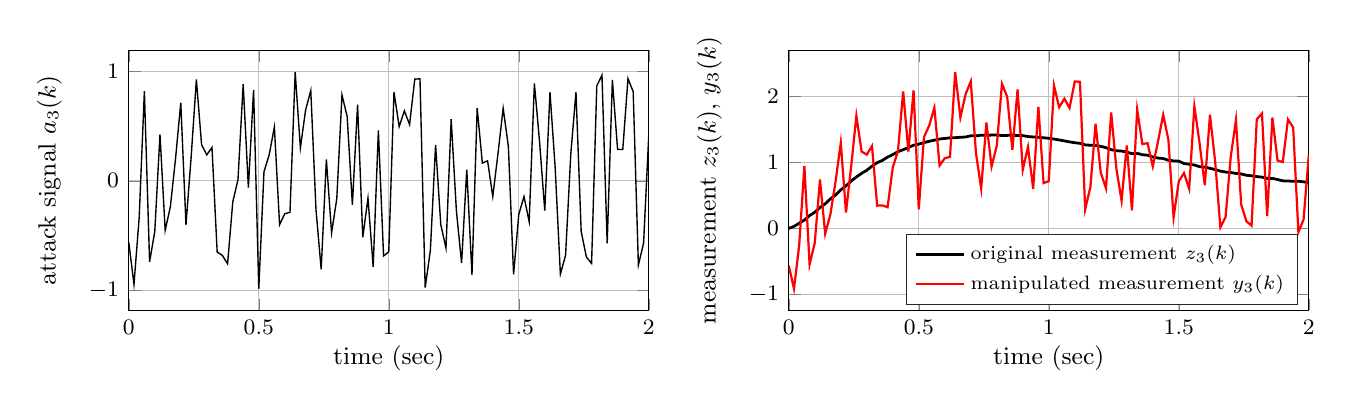
\begin{tikzpicture}
\begin{axis}
[	width=2.6in,
	height=1.3in,
	at={(0in,1.7in)},
	scale only axis,
	xmin=0,
	xmax=2.0,
	xlabel={\small time (sec)},
	ylabel={\small attack signal $a_3(k)$},
	x label style={at={(axis description cs:0.5,-0.1)},anchor=north},
	y label style={at={(axis description cs:-0.11,.5)},anchor=south},
	xticklabel style = {font=\footnotesize},
	yticklabel style = {font=\footnotesize},
	axis background/.style={fill=white},
	xmajorgrids,
	ymajorgrids,
	legend style={at={(0.98,0.02)}, anchor=south east, legend cell align=left, align=left, draw=white!15!black, font=\scriptsize}]
	 \addplot [color={black}, line width=0.5pt]
	table[row sep={\\}]
	{
0.0  -0.5625685225246384  \\
0.02  -0.946157670457147  \\
0.04  -0.3364104982135254  \\
0.06  0.8202072091057051  \\
0.08  -0.7416794304773182  \\
0.1  -0.4636695887925457  \\
0.12  0.4247375003814464  \\
0.14  -0.4529398288478932  \\
0.16  -0.23609426388419186  \\
0.18  0.20607156940463156  \\
0.2  0.7146776978338217  \\
0.22  -0.4031811551171538  \\
0.24  0.2206252826036046  \\
0.26  0.9264480578446211  \\
0.28  0.33016511715381247  \\
0.3  0.23718509653538966  \\
0.32  0.3053190945443012  \\
0.34  -0.6512496890635018  \\
0.36  -0.6822150171560071  \\
0.38  -0.7591862879712541  \\
0.4  -0.19280907417578508  \\
0.42  0.010038743472394973  \\
0.44  0.8827731819816345  \\
0.46  -0.06232326649906916  \\
0.48  0.8319345169225183  \\
0.5  -0.9872827034407057  \\
0.52  0.08252119515841416  \\
0.54  0.23761861917437788  \\
0.56  0.4911335147891096  \\
0.58  -0.40195620239799457  \\
0.6  -0.3007915416907321  \\
0.62  -0.2880389885558321  \\
0.64  0.9936238737504954  \\
0.66  0.301057855330896  \\
0.68  0.6458920116460922  \\
0.7  0.825439900787106  \\
0.72  -0.2620778554704919  \\
0.74  -0.8099631243406966  \\
0.76  0.19437015142373726  \\
0.78  -0.4755865591670845  \\
0.8  -0.16394509461018458  \\
0.82  0.7845865898376772  \\
0.84  0.5867174223091793  \\
0.86  -0.2193032349255386  \\
0.88  0.6958595916418464  \\
0.9  -0.5164339756771317  \\
0.92  -0.15836646301569557  \\
0.94  -0.7857843469695074  \\
0.96  0.46132582292170277  \\
0.98  -0.6869516269713491  \\
1.0  -0.6493852750653204  \\
1.02  0.8112005067738504  \\
1.04  0.49552013490097657  \\
1.06  0.6395260827687634  \\
1.08  0.5144317327991712  \\
1.1  0.9294456667948578  \\
1.12  0.9324288820292381  \\
1.14  -0.9769366346964161  \\
1.16  -0.6351510189600362  \\
1.18  0.32726158838108965  \\
1.2  -0.40098100760181365  \\
1.22  -0.6150064270922488  \\
1.24  0.5641016529988976  \\
1.26  -0.27231215515339535  \\
1.28  -0.752554332947537  \\
1.3  0.10187427646239922  \\
1.32  -0.8600011844841662  \\
1.34  0.6642700257000524  \\
1.36  0.16170120198315496  \\
1.38  0.1826664933681159  \\
1.4  -0.14334483866806247  \\
1.42  0.2486222622627241  \\
1.44  0.6622426969022284  \\
1.46  0.3136861979015393  \\
1.48  -0.8557620863445856  \\
1.5  -0.3070342555493415  \\
1.52  -0.14416760270375484  \\
1.54  -0.37368830515195883  \\
1.56  0.8911874844829586  \\
1.58  0.35518376316127453  \\
1.6  -0.27339031973850947  \\
1.62  0.8105521223144891  \\
1.64  0.11784059265095037  \\
1.66  -0.8529040350736259  \\
1.68  -0.6806944273502968  \\
1.7  0.24363510423789958  \\
1.72  0.8110402429453711  \\
1.74  -0.4624898957872765  \\
1.76  -0.6967699885218077  \\
1.78  -0.7555009870069109  \\
1.8  0.8677999951918474  \\
1.82  0.9651388566369782  \\
1.84  -0.572692343156155  \\
1.86  0.9214722802132305  \\
1.88  0.28714732919033314  \\
1.9  0.28600006541082534  \\
1.92  0.9336419255406856  \\
1.94  0.8153373412752746  \\
1.96  -0.771121795555112  \\
1.98  -0.5703813934558002  \\
2.0  0.4202296393480983  \\
	};
	

\end{axis}

\begin{axis}
[	width=2.6in,
height=1.3in,
at={(3.3in,1.7in)},
scale only axis,
xmin=0,
xmax=2.0,
xlabel={\small time (sec)},
ylabel={\small measurement $z_3(k)$, $y_3(k)$},
x label style={at={(axis description cs:0.5,-0.1)},anchor=north},
y label style={at={(axis description cs:-0.11,.5)},anchor=south},
xticklabel style = {font=\footnotesize},
yticklabel style = {font=\footnotesize},
axis background/.style={fill=white},
xmajorgrids,
ymajorgrids,
legend style={at={(0.98,0.02)}, anchor=south east, legend cell align=left, align=left, draw=white!15!black, font=\scriptsize}]
\addplot [color={black}, line width=1pt]
table[row sep={\\}]
{
	0.0  0.0005061476188890966  \\
	0.02  0.031676588671764164  \\
	0.04  0.07839140216717005  \\
	0.06  0.12705814413038907  \\
	0.08  0.19480431491342415  \\
	0.1  0.24606443660984756  \\
	0.12  0.3172084112413346  \\
	0.14  0.3736461521457517  \\
	0.16  0.44787503073264906  \\
	0.18  0.5069223027691104  \\
	0.2  0.5852364000596318  \\
	0.22  0.6450996948371481  \\
	0.24  0.719598187094292  \\
	0.26  0.7802246068858262  \\
	0.28  0.8352976511484314  \\
	0.3  0.8819249843701404  \\
	0.32  0.9438334235786126  \\
	0.34  0.9968137130862087  \\
	0.36  1.0315121996566714  \\
	0.38  1.081352724577131  \\
	0.4  1.1186852002911756  \\
	0.42  1.1641077812910212  \\
	0.44  1.1939659134273448  \\
	0.46  1.2272556361330376  \\
	0.48  1.261665715825486  \\
	0.5  1.2786078316998268  \\
	0.52  1.3011683448134117  \\
	0.54  1.321384821506629  \\
	0.56  1.338382036174266  \\
	0.58  1.355281400342649  \\
	0.6  1.3648091021791213  \\
	0.62  1.3732953101805965  \\
	0.64  1.3762112690389299  \\
	0.66  1.382112031788601  \\
	0.68  1.3860206445448202  \\
	0.7  1.4048404930230238  \\
	0.72  1.4039269899470739  \\
	0.74  1.4137690804441447  \\
	0.76  1.4113935296580151  \\
	0.78  1.415466288691426  \\
	0.8  1.4173504637099132  \\
	0.82  1.408216099780143  \\
	0.84  1.410853101252453  \\
	0.86  1.4122366732375526  \\
	0.88  1.4099148151176653  \\
	0.9  1.4068220459084428  \\
	0.92  1.3932771447410874  \\
	0.94  1.3869197810882306  \\
	0.96  1.3816719911696593  \\
	0.98  1.3746540193141819  \\
	1.0  1.3668281178807369  \\
	1.02  1.3552820898141782  \\
	1.04  1.3412950137254243  \\
	1.06  1.327392873379449  \\
	1.08  1.312190740537211  \\
	1.1  1.2995220178320626  \\
	1.12  1.290181413888831  \\
	1.14  1.2667219743156652  \\
	1.16  1.2612298991666215  \\
	1.18  1.2589715517767963  \\
	1.2  1.2447068247074753  \\
	1.22  1.2246558090903343  \\
	1.24  1.1947392767545253  \\
	1.26  1.178691587432372  \\
	1.28  1.1725210952749316  \\
	1.3  1.1574143114167688  \\
	1.32  1.1333554895621063  \\
	1.34  1.1379319746939296  \\
	1.36  1.1176217433173101  \\
	1.38  1.1102593716696092  \\
	1.4  1.0836873054208704  \\
	1.42  1.067036714947158  \\
	1.44  1.0605533729454986  \\
	1.46  1.0344992068703907  \\
	1.48  1.0243303238705184  \\
	1.5  1.020077500634661  \\
	1.52  0.9839768264319667  \\
	1.54  0.973260433229496  \\
	1.56  0.9617053886606732  \\
	1.58  0.936138032340902  \\
	1.6  0.9293793225658402  \\
	1.62  0.9117291638631297  \\
	1.64  0.8920858206651604  \\
	1.66  0.8695958676647998  \\
	1.68  0.8548008571060354  \\
	1.7  0.8475448183415518  \\
	1.72  0.8342039556123342  \\
	1.74  0.8264765990017806  \\
	1.76  0.806244182872368  \\
	1.78  0.798659029368042  \\
	1.8  0.7863949401958488  \\
	1.82  0.7781995154823723  \\
	1.84  0.7591860534071165  \\
	1.86  0.7588840404102928  \\
	1.88  0.7418834336133863  \\
	1.9  0.7215463501855689  \\
	1.92  0.7193921889269146  \\
	1.94  0.714570339094586  \\
	1.96  0.7160728188691623  \\
	1.98  0.7071802256678278  \\
	2.0  0.6911892058577479  \\
}
;\addlegendentry{original measurement $z_3(k)$}

\addplot [color={red}, line width=0.8pt]
table[row sep={\\}]
{
   0.0  -0.5620623749057493  \\
0.02  -0.9144810817853829  \\
0.04  -0.25801909604635537  \\
0.06  0.9472653532360942  \\
0.08  -0.546875115563894  \\
0.1  -0.21760515218269816  \\
0.12  0.741945911622781  \\
0.14  -0.07929367670214149  \\
0.16  0.2117807668484572  \\
0.18  0.712993872173742  \\
0.2  1.2999140978934536  \\
0.22  0.24191853971999433  \\
0.24  0.9402234696978966  \\
0.26  1.7066726647304473  \\
0.28  1.1654627683022438  \\
0.3  1.11911008090553  \\
0.32  1.2491525181229137  \\
0.34  0.3455640240227069  \\
0.36  0.3492971825006643  \\
0.38  0.32216643660587696  \\
0.4  0.9258761261153905  \\
0.42  1.1741465247634162  \\
0.44  2.0767390954089793  \\
0.46  1.1649323696339684  \\
0.48  2.0936002327480043  \\
0.5  0.29132512825912116  \\
0.52  1.3836895399718259  \\
0.54  1.559003440681007  \\
0.56  1.8295155509633756  \\
0.58  0.9533251979446544  \\
0.6  1.0640175604883892  \\
0.62  1.0852563216247644  \\
0.64  2.3698351427894253  \\
0.66  1.683169887119497  \\
0.68  2.0319126561909124  \\
0.7  2.23028039381013  \\
0.72  1.141849134476582  \\
0.74  0.6038059561034481  \\
0.76  1.6057636810817524  \\
0.78  0.9398797295243415  \\
0.8  1.2534053690997287  \\
0.82  2.19280268961782  \\
0.84  1.9975705235616323  \\
0.86  1.192933438312014  \\
0.88  2.1057744067595117  \\
0.9  0.8903880702313112  \\
0.92  1.2349106817253919  \\
0.94  0.6011354341187232  \\
0.96  1.842997814091362  \\
0.98  0.6877023923428327  \\
1.0  0.7174428428154165  \\
1.02  2.1664825965880286  \\
1.04  1.8368151486264008  \\
1.06  1.9669189561482123  \\
1.08  1.8266224733363823  \\
1.1  2.2289676846269204  \\
1.12  2.222610295918069  \\
1.14  0.2897853396192491  \\
1.16  0.6260788802065853  \\
1.18  1.586233140157886  \\
1.2  0.8437258171056616  \\
1.22  0.6096493819980855  \\
1.24  1.7588409297534229  \\
1.26  0.9063794322789767  \\
1.28  0.4199667623273946  \\
1.3  1.259288587879168  \\
1.32  0.2733543050779401  \\
1.34  1.802202000393982  \\
1.36  1.279322945300465  \\
1.38  1.292925865037725  \\
1.4  0.940342466752808  \\
1.42  1.3156589772098821  \\
1.44  1.722796069847727  \\
1.46  1.34818540477193  \\
1.48  0.16856823752593275  \\
1.5  0.7130432450853195  \\
1.52  0.8398092237282119  \\
1.54  0.5995721280775371  \\
1.56  1.8528928731436318  \\
1.58  1.2913217955021765  \\
1.6  0.6559890028273307  \\
1.62  1.7222812861776189  \\
1.64  1.0099264133161108  \\
1.66  0.016691832591173905  \\
1.68  0.17410642975573853  \\
1.7  1.0911799225794514  \\
1.72  1.6452441985577053  \\
1.74  0.3639867032145041  \\
1.76  0.10947419435056027  \\
1.78  0.04315804236113108  \\
1.8  1.6541949353876961  \\
1.82  1.7433383721193505  \\
1.84  0.1864937102509615  \\
1.86  1.6803563206235232  \\
1.88  1.0290307628037194  \\
1.9  1.0075464155963942  \\
1.92  1.6530341144676002  \\
1.94  1.5299076803698606  \\
1.96  -0.05504897668594966  \\
1.98  0.1367988322120276  \\
2.0  1.1114188452058462  \\
}
;\addlegendentry{{manipulated measurement $y_3(k)$}}


\end{axis}

%  	\begin{axis}
%	[	width=2.6in,
%	height=1.3in,
%	at={(0in,0in)},
%	scale only axis,
%	xmin=0,
%	xmax=2.0,
%%	ymin=-4,
%%	ymax=2,
%	xlabel={\small time (sec)},
%	ylabel={\small $x_3$ pendulumn angle},
%	x label style={at={(axis description cs:0.5,-0.1)},anchor=north},
%	y label style={at={(axis description cs:-0.11,.5)},anchor=south},
%	xticklabel style = {font=\footnotesize},
%	yticklabel style = {font=\footnotesize},
%	axis background/.style={fill=white},
%	xmajorgrids,
%	ymajorgrids,
%	legend style={at={(0.98,0.02)}, anchor=south east, legend cell align=left, align=left, draw=white!15!black, font=\scriptsize}]
%	\addplot [color={black}, line width=1pt]
%	table[row sep={\\}]
%	{
%0.0  0.0  \\
%0.02  0.00772853593415913  \\
%0.04  0.004801671416923327  \\
%0.06  -0.012528997431996048  \\
%0.08  -0.034478619332425936  \\
%0.1  -0.06220231524500317  \\
%0.12  -0.08812635048651297  \\
%0.14  -0.11408845091735348  \\
%0.16  -0.14488997218330013  \\
%0.18  -0.16947348245078697  \\
%0.2  -0.19501471373927462  \\
%0.22  -0.2166030568036244  \\
%0.24  -0.23694887645664164  \\
%0.26  -0.2534179553657174  \\
%0.28  -0.2659048131170473  \\
%0.3  -0.2814074322954603  \\
%0.32  -0.2947651384686937  \\
%0.34  -0.30280625979339526  \\
%0.36  -0.3110461733895194  \\
%0.38  -0.322599925444607  \\
%0.4  -0.3266601375700984  \\
%0.42  -0.32832183302190043  \\
%0.44  -0.33079378651792585  \\
%0.46  -0.33139999061403563  \\
%0.48  -0.33190912976035625  \\
%0.5  -0.32830514918189446  \\
%0.52  -0.3265624628054656  \\
%0.54  -0.3231032971609128  \\
%0.56  -0.31943423376946206  \\
%0.58  -0.31567219360956844  \\
%0.6  -0.3139459878003922  \\
%0.62  -0.30858429971742735  \\
%0.64  -0.302866065490615  \\
%0.66  -0.2975240107704187  \\
%0.68  -0.29156813130488785  \\
%0.7  -0.28705864201984305  \\
%0.72  -0.2800613967051828  \\
%0.74  -0.2721345042496352  \\
%0.76  -0.2675647476463787  \\
%0.78  -0.26004373544306775  \\
%0.8  -0.24895562242482422  \\
%0.82  -0.24469615255703123  \\
%0.84  -0.23679296240647962  \\
%0.86  -0.22526462977535064  \\
%0.88  -0.21530137387528134  \\
%0.9  -0.2019610820610649  \\
%0.92  -0.19283115640996426  \\
%0.94  -0.18404650174938508  \\
%0.96  -0.1761938176509628  \\
%0.98  -0.16952154188571567  \\
%1.0  -0.16068318494400077  \\
%1.02  -0.15115385465801076  \\
%1.04  -0.142077499764086  \\
%1.06  -0.13285231555738442  \\
%1.08  -0.12217488148841449  \\
%1.1  -0.11717625074624005  \\
%1.12  -0.11014342489808715  \\
%1.14  -0.10290962697247244  \\
%1.16  -0.09707223606283309  \\
%1.18  -0.08535583686102192  \\
%1.2  -0.07985586728850495  \\
%1.22  -0.07053290137389215  \\
%1.24  -0.0660756875734225  \\
%1.26  -0.05925950423578198  \\
%1.28  -0.04983238664926049  \\
%1.3  -0.046321730532286276  \\
%1.32  -0.04111947230774583  \\
%1.34  -0.03716014124124552  \\
%1.36  -0.026958173254637667  \\
%1.38  -0.02105479624823502  \\
%1.4  -0.013204082238369545  \\
%1.42  -0.007208612852129617  \\
%1.44  -0.005029793064317797  \\
%1.46  -0.0030365387904538444  \\
%1.48  -0.004685191023569348  \\
%1.5  -0.0013502134977833556  \\
%1.52  -0.0012637857934116841  \\
%1.54  -0.0012840803221537893  \\
%1.56  0.004161592495718868  \\
%1.58  0.007337270321035059  \\
%1.6  0.007873265952081725  \\
%1.62  0.007756595504494869  \\
%1.64  0.012948213825993315  \\
%1.66  0.01713997304166258  \\
%1.68  0.019303428528959714  \\
%1.7  0.021720664071569973  \\
%1.72  0.021496525088056485  \\
%1.74  0.02269954427453162  \\
%1.76  0.025127263635035712  \\
%1.78  0.025581388241573386  \\
%1.8  0.022956371536018347  \\
%1.82  0.020320909246699284  \\
%1.84  0.02325727363447171  \\
%1.86  0.022566429135964905  \\
%1.88  0.025410932971556357  \\
%1.9  0.025581397517493814  \\
%1.92  0.024133015365711413  \\
%1.94  0.024607306183292644  \\
%1.96  0.02686997993370564  \\
%1.98  0.028618584557972122  \\
%2.0  0.02949612536857937  \\
%	}
%	;\addlegendentry{state $x_3$}
%	\addplot [color={red},dashed, line width=1pt]
%	table[row sep={\\}]
%	{
%	 0.0  0.0  \\
%	0.02  0.00809402453328914  \\
%	0.04  0.002283710058266839  \\
%	0.06  -0.011924222353404363  \\
%	0.08  -0.03538807548199385  \\
%	0.1  -0.062495688561897404  \\
%	0.12  -0.08979727756857352  \\
%	0.14  -0.11596912737252132  \\
%	0.16  -0.14427298978459968  \\
%	0.18  -0.1699091880689923  \\
%	0.2  -0.19571409358693093  \\
%	0.22  -0.21710723871475957  \\
%	0.24  -0.23750518798723996  \\
%	0.26  -0.2523487237267693  \\
%	0.28  -0.26564551359739796  \\
%	0.3  -0.28113924184632594  \\
%	0.32  -0.29344313265186917  \\
%	0.34  -0.30387742299429843  \\
%	0.36  -0.31093266172634626  \\
%	0.38  -0.32032314034771303  \\
%	0.4  -0.32488432492231156  \\
%	0.42  -0.328256133800731  \\
%	0.44  -0.33170684466667966  \\
%	0.46  -0.33284554813223155  \\
%	0.48  -0.32934060251669267  \\
%	0.5  -0.32881415681358606  \\
%	0.52  -0.32672393145274836  \\
%	0.54  -0.3217023284966502  \\
%	0.56  -0.31920782046530927  \\
%	0.58  -0.3155857583713461  \\
%	0.6  -0.31200171978648444  \\
%	0.62  -0.30753884981430435  \\
%	0.64  -0.30328744734313084  \\
%	0.66  -0.298819639225292  \\
%	0.68  -0.2916263924411364  \\
%	0.7  -0.2838538399639527  \\
%	0.72  -0.27822533107121034  \\
%	0.74  -0.27214850374295424  \\
%	0.76  -0.2649862125224101  \\
%	0.78  -0.2581935349054245  \\
%	0.8  -0.24687375692743166  \\
%	0.82  -0.24215334598492766  \\
%	0.84  -0.23463968652823464  \\
%	0.86  -0.2266454648618093  \\
%	0.88  -0.21570653361944153  \\
%	0.9  -0.20378113555698663  \\
%	0.92  -0.1922094272504351  \\
%	0.94  -0.18193892229656553  \\
%	0.96  -0.17462306148804935  \\
%	0.98  -0.16857998362472904  \\
%	1.0  -0.1589098101915298  \\
%	1.02  -0.1502282447377052  \\
%	1.04  -0.14310208638808308  \\
%	1.06  -0.13391428982914821  \\
%	1.08  -0.12206666034954945  \\
%	1.1  -0.11753381580332939  \\
%	1.12  -0.11064111898353321  \\
%	1.14  -0.10215982660161821  \\
%	1.16  -0.096618902112179  \\
%	1.18  -0.08817640412095815  \\
%	1.2  -0.07931844432254224  \\
%	1.22  -0.0713170158403937  \\
%	1.24  -0.06598326032462205  \\
%	1.26  -0.05869782541506201  \\
%	1.28  -0.05244831403760163  \\
%	1.3  -0.04689123976106053  \\
%	1.32  -0.04325454089798624  \\
%	1.34  -0.03885220256504527  \\
%	1.36  -0.030517495413270805  \\
%	1.38  -0.024466342268987945  \\
%	1.4  -0.018729185184462  \\
%	1.42  -0.010157661361933055  \\
%	1.44  -0.005799650225733364  \\
%	1.46  -0.0017710381011364653  \\
%	1.48  -0.002224799382994183  \\
%	1.5  -0.0037629560253844437  \\
%	1.52  -0.00020440203585928116  \\
%	1.54  0.0012643359647233753  \\
%	1.56  0.003252784378121404  \\
%	1.58  0.005266412443152401  \\
%	1.6  0.006949937595322902  \\
%	1.62  0.008256452575278935  \\
%	1.64  0.012007453507124496  \\
%	1.66  0.01615310418726861  \\
%	1.68  0.019000666804788804  \\
%	1.7  0.022087371511188413  \\
%	1.72  0.022261092399250972  \\
%	1.74  0.02355749395802008  \\
%	1.76  0.023895346270558754  \\
%	1.78  0.026333022304786253  \\
%	1.8  0.02456626556539792  \\
%	1.82  0.021605386228436392  \\
%	1.84  0.023528349423668403  \\
%	1.86  0.023572743261476937  \\
%	1.88  0.025126899283551846  \\
%	1.9  0.025833933274513415  \\
%	1.92  0.02280935517999988  \\
%	1.94  0.025189469054832925  \\
%	1.96  0.02661138935665535  \\
%	1.98  0.02763011362829756  \\
%	2.0  0.027469141828147026  \\
%	}
%	;\addlegendentry{{ Kalman estimation $\hat{x}_3$}}
%	\addplot[densely dotted, color={blue}, line width=1pt]
%	table[row sep={\\}]
%	{
%    0.0  1.8153964737662312e-5  \\
%0.02  0.0066894619554046355  \\
%0.04  0.0018375871994040162  \\
%0.06  -0.011012697570773474  \\
%0.08  -0.03609804873935931  \\
%0.1  -0.06340645502442915  \\
%0.12  -0.0895457918792631  \\
%0.14  -0.11546107462068377  \\
%0.16  -0.14461477831571443  \\
%0.18  -0.17007154514361927  \\
%0.2  -0.1965051643232883  \\
%0.22  -0.2166340902306285  \\
%0.24  -0.23770039325448397  \\
%0.26  -0.2507335125541037  \\
%0.28  -0.2645156857629006  \\
%0.3  -0.28216527675191616  \\
%0.32  -0.2939902057265568  \\
%0.34  -0.30440857374041375  \\
%0.36  -0.31047444062583235  \\
%0.38  -0.32198495278139255  \\
%0.4  -0.3249118700086211  \\
%0.42  -0.32841640163734204  \\
%0.44  -0.33251010788936297  \\
%0.46  -0.3331188005365526  \\
%0.48  -0.32767165979082796  \\
%0.5  -0.3288637216034393  \\
%0.52  -0.3265504673964966  \\
%0.54  -0.3205275268798475  \\
%0.56  -0.3197884422608594  \\
%0.58  -0.3157679939079811  \\
%0.6  -0.31254421435944685  \\
%0.62  -0.30806083114358135  \\
%0.64  -0.3038352148338218  \\
%0.66  -0.2994116819525727  \\
%0.68  -0.29121889287466646  \\
%0.7  -0.2833617882231757  \\
%0.72  -0.27936861590095097  \\
%0.74  -0.27290542088826425  \\
%0.76  -0.2654318394097727  \\
%0.78  -0.25942935600796185  \\
%0.8  -0.2457658293296008  \\
%0.82  -0.24403414344605018  \\
%0.84  -0.2358616914531913  \\
%0.86  -0.2275077308550984  \\
%0.88  -0.21485981313066116  \\
%0.9  -0.20232178782749977  \\
%0.92  -0.19104608352709898  \\
%0.94  -0.18111885006671183  \\
%0.96  -0.1754534261052666  \\
%0.98  -0.17003134488456753  \\
%1.0  -0.15878283143959224  \\
%1.02  -0.15051065091807594  \\
%1.04  -0.1435009071579159  \\
%1.06  -0.13363074186982313  \\
%1.08  -0.12038778178826819  \\
%1.1  -0.11866338138681089  \\
%1.12  -0.110930248968576  \\
%1.14  -0.10181163345285733  \\
%1.16  -0.09751700179946482  \\
%1.18  -0.08758702035485068  \\
%1.2  -0.07785509840417323  \\
%1.22  -0.07050311362538186  \\
%1.24  -0.06601841440192815  \\
%1.26  -0.05793710743206526  \\
%1.28  -0.051999353311811235  \\
%1.3  -0.04693730475850037  \\
%1.32  -0.04389217870983184  \\
%1.34  -0.038972560152190514  \\
%1.36  -0.02865888152011623  \\
%1.38  -0.02353592133370778  \\
%1.4  -0.017640744192343967  \\
%1.42  -0.007667707763960579  \\
%1.44  -0.004952961222438092  \\
%1.46  -0.0008037137317556581  \\
%1.48  -0.003445327891030425  \\
%1.5  -0.005518722706033974  \\
%1.52  0.0004546477429451413  \\
%1.54  0.0010515168391628813  \\
%1.56  0.0032978681139044274  \\
%1.58  0.005456467908684386  \\
%1.6  0.007016058115342972  \\
%1.62  0.007992613905111441  \\
%1.64  0.013215471326015648  \\
%1.66  0.01730891328170967  \\
%1.68  0.01980891940823777  \\
%1.7  0.023250483613783467  \\
%1.72  0.02194819975361911  \\
%1.74  0.023940958356646756  \\
%1.76  0.023721571245686246  \\
%1.78  0.027350023652804832  \\
%1.8  0.023546924861985615  \\
%1.82  0.019857344070720775  \\
%1.84  0.023909886569047793  \\
%1.86  0.0231294380862511  \\
%1.88  0.02574352864188202  \\
%1.9  0.025842587721728108  \\
%1.92  0.02092146538831675  \\
%1.94  0.025931184643444655  \\
%1.96  0.027084411024922466  \\
%1.98  0.027575839585923738  \\
%2.0  0.026971498895954696  \\
%	}
%;\addlegendentry{{our estimation $\tilde{x}_3$}}
%
%
%\end{axis}
%
%\begin{axis}
%[	width=2.6in,
%height=1.3in,
%at={(3.3in,0in)},
%scale only axis,
%xmin=0,
%xmax=2.0,
%%ymin=-4,
%%ymax=2,
%xlabel={\small time (sec)},
%ylabel={\small $x_4$ pendulumn angle velocity},
%x label style={at={(axis description cs:0.5,-0.1)},anchor=north},
%y label style={at={(axis description cs:-0.11,.5)},anchor=south},
%xticklabel style = {font=\footnotesize},
%yticklabel style = {font=\footnotesize},
%axis background/.style={fill=white},
%xmajorgrids,
%ymajorgrids,
%legend style={at={(0.98,0.02)}, anchor=south east, legend cell align=left, align=left, draw=white!15!black, font=\scriptsize}]
%\addplot [color={black}, line width=1pt]
%table[row sep={\\}]
%{
%  0.0  1.0  \\
%0.02  0.05313305390126177  \\
%0.04  -0.5807597079886778  \\
%0.06  -0.9849649892184913  \\
%0.08  -1.2236616544745775  \\
%0.1  -1.3448708265564777  \\
%0.12  -1.3911973425235322  \\
%0.14  -1.3847017109780744  \\
%0.16  -1.3360588370385862  \\
%0.18  -1.2612956960549269  \\
%0.2  -1.1712121233640451  \\
%0.22  -1.071999578445813  \\
%0.24  -0.9674797110228057  \\
%0.26  -0.8680549183886634  \\
%0.28  -0.7699884280336178  \\
%0.3  -0.6746842796248621  \\
%0.32  -0.586875654761506  \\
%0.34  -0.4959299174041296  \\
%0.36  -0.40597661697079446  \\
%0.38  -0.32771095994654365  \\
%0.4  -0.253961547290701  \\
%0.42  -0.18263871652089975  \\
%0.44  -0.11573407741218594  \\
%0.46  -0.05911515161120641  \\
%0.48  0.0009801138197992887  \\
%0.5  0.04463813200237973  \\
%0.52  0.09038368590143643  \\
%0.54  0.12381466371390598  \\
%0.56  0.16193471899976158  \\
%0.58  0.19217803962499197  \\
%0.6  0.2284585486584002  \\
%0.62  0.27315223526991256  \\
%0.64  0.3029744279918313  \\
%0.66  0.3360381761463694  \\
%0.68  0.36405311581028843  \\
%0.7  0.3862145241118462  \\
%0.72  0.4052381391063923  \\
%0.74  0.40659407112164414  \\
%0.76  0.4016463115722345  \\
%0.78  0.39680426743202124  \\
%0.8  0.3921338510569967  \\
%0.82  0.3884591608505884  \\
%0.84  0.3897778445333768  \\
%0.86  0.3978434385510643  \\
%0.88  0.40888248291393214  \\
%0.9  0.40349125898703586  \\
%0.92  0.4043181979298124  \\
%0.94  0.4001713487291486  \\
%0.96  0.397537790317619  \\
%0.98  0.3906342747298136  \\
%1.0  0.377882856254513  \\
%1.02  0.3727858562415341  \\
%1.04  0.3579748382263377  \\
%1.06  0.34457979003538486  \\
%1.08  0.3274365776280705  \\
%1.1  0.31223393396172927  \\
%1.12  0.2972605478138003  \\
%1.14  0.28374482940224277  \\
%1.16  0.27808313315371463  \\
%1.18  0.2752540519763583  \\
%1.2  0.27226461109496636  \\
%1.22  0.27696110635321103  \\
%1.24  0.26990768271144283  \\
%1.26  0.26054532527838425  \\
%1.28  0.2504740216554849  \\
%1.3  0.24312004848395827  \\
%1.32  0.24828658502523776  \\
%1.34  0.2471687742404289  \\
%1.36  0.2483512476352048  \\
%1.38  0.2421106054905815  \\
%1.4  0.2281155213543221  \\
%1.42  0.2192043397969218  \\
%1.44  0.21813440821530206  \\
%1.46  0.215847499113375  \\
%1.48  0.21810640903792972  \\
%1.5  0.21793606071633792  \\
%1.52  0.21839791991053367  \\
%1.54  0.21094224607272868  \\
%1.56  0.20175648284456538  \\
%1.58  0.18577552098976302  \\
%1.6  0.17234252915874954  \\
%1.62  0.1667589628096436  \\
%1.64  0.16336600936391402  \\
%1.66  0.15026901018454916  \\
%1.68  0.1427360828668787  \\
%1.7  0.13367410170858618  \\
%1.72  0.12734499958354706  \\
%1.74  0.11405351681196844  \\
%1.76  0.10587244286568445  \\
%1.78  0.10156266429081387  \\
%1.8  0.0936679758808678  \\
%1.82  0.08822122445956102  \\
%1.84  0.07018133601995245  \\
%1.86  0.05094537909202273  \\
%1.88  0.04130087142500513  \\
%1.9  0.032313361980953  \\
%1.92  0.02866897811479254  \\
%1.94  0.030018199155337016  \\
%1.96  0.029179914657290675  \\
%1.98  0.029178093401201616  \\
%2.0  0.02640041419686011  \\
%}
%;\addlegendentry{state $x_4$}
%\addplot [color={red},dashed, line width=1pt]
%table[row sep={\\}]
%{
%0.0  1.0  \\
%0.02  0.05196229099537668  \\
%0.04  -0.5824313535988286  \\
%0.06  -0.9891377715191895  \\
%0.08  -1.225040556372666  \\
%0.1  -1.3474376677420603  \\
%0.12  -1.3927650448471267  \\
%0.14  -1.3853875418228592  \\
%0.16  -1.3385535189542455  \\
%0.18  -1.2616908106226903  \\
%0.2  -1.1733481356619362  \\
%0.22  -1.0733971982561636  \\
%0.24  -0.9709048883726853  \\
%0.26  -0.8734509930998627  \\
%0.28  -0.7737477786715035  \\
%0.3  -0.6814462079764667  \\
%0.32  -0.5930068323706987  \\
%0.34  -0.5011111690344067  \\
%0.36  -0.4117486708366517  \\
%0.38  -0.32787217975647187  \\
%0.4  -0.25500615240975977  \\
%0.42  -0.18223637558459482  \\
%0.44  -0.1136859116043202  \\
%0.46  -0.05435490540626656  \\
%0.48  0.001052155333388885  \\
%0.5  0.047862836014496535  \\
%0.52  0.09307612385402939  \\
%0.54  0.12661541422593295  \\
%0.56  0.16673898540858903  \\
%0.58  0.20040364092746082  \\
%0.6  0.2378257684031066  \\
%0.62  0.28092995786664526  \\
%0.64  0.30722850104675375  \\
%0.66  0.33988761950874746  \\
%0.68  0.3717014698259486  \\
%0.7  0.39114473419457757  \\
%0.72  0.41074056965705785  \\
%0.74  0.4157082365437478  \\
%0.76  0.4107206907578836  \\
%0.78  0.40479797621004415  \\
%0.8  0.4002479612239634  \\
%0.82  0.39670525295180864  \\
%0.84  0.402980720989716  \\
%0.86  0.40966660580558506  \\
%0.88  0.41939855229643713  \\
%0.9  0.4136774603389678  \\
%0.92  0.41337706589827294  \\
%0.94  0.4076360923733703  \\
%0.96  0.40419133912255345  \\
%0.98  0.39738214224816115  \\
%1.0  0.38613613596819135  \\
%1.02  0.37863833492291044  \\
%1.04  0.3613171630485197  \\
%1.06  0.34817084130208276  \\
%1.08  0.3337665386001098  \\
%1.1  0.322513876054837  \\
%1.12  0.30951293238535926  \\
%1.14  0.29822140789925367  \\
%1.16  0.2887209415996951  \\
%1.18  0.2855447198327156  \\
%1.2  0.2792019100681843  \\
%1.22  0.28259480121327957  \\
%1.24  0.27674766540821855  \\
%1.26  0.2679337895584435  \\
%1.28  0.25957147095312993  \\
%1.3  0.2512852868921737  \\
%1.32  0.25335034594023265  \\
%1.34  0.2517049563980485  \\
%1.36  0.24854241554762116  \\
%1.38  0.2437570887642059  \\
%1.4  0.232081337423728  \\
%1.42  0.2246763936573522  \\
%1.44  0.22593853025256636  \\
%1.46  0.22180580292165525  \\
%1.48  0.2201777881736648  \\
%1.5  0.21772174841998373  \\
%1.52  0.22039359761167476  \\
%1.54  0.21451665272588324  \\
%1.56  0.20671496543671092  \\
%1.58  0.19237907013470915  \\
%1.6  0.17849341727408496  \\
%1.62  0.1693669711801831  \\
%1.64  0.1654694365161853  \\
%1.66  0.15476608715270937  \\
%1.68  0.14644491458503275  \\
%1.7  0.1380087312073818  \\
%1.72  0.12999696162763208  \\
%1.74  0.11642996712779241  \\
%1.76  0.10651977489569771  \\
%1.78  0.09914327961373791  \\
%1.8  0.09326070775598083  \\
%1.82  0.08760116773835838  \\
%1.84  0.07441328030636729  \\
%1.86  0.0534154762075595  \\
%1.88  0.04537417203289343  \\
%1.9  0.03311477519912949  \\
%1.92  0.029386264188961075  \\
%1.94  0.031449452742925314  \\
%1.96  0.028203792066178256  \\
%1.98  0.026902194874244584  \\
%2.0  0.023968301890876745  \\
%}
%;\addlegendentry{{ Kalman estimation $\hat{x}_4$}}
%\addplot[densely dotted, color={blue}, line width=1pt]
%table[row sep={\\}]
%{
%   0.0  0.9999999995931783  \\
%0.02  0.053256438469400355  \\
%0.04  -0.5810558367590097  \\
%0.06  -0.9888797959421549  \\
%0.08  -1.223881505907738  \\
%0.1  -1.3453082018539748  \\
%0.12  -1.3891303460776288  \\
%0.14  -1.379673068887711  \\
%0.16  -1.3337025957314825  \\
%0.18  -1.253342000372752  \\
%0.2  -1.165825320019194  \\
%0.22  -1.0647406851480974  \\
%0.24  -0.962864368017885  \\
%0.26  -0.8669013996514804  \\
%0.28  -0.7648147896002787  \\
%0.3  -0.6716102653407486  \\
%0.32  -0.5837308230993299  \\
%0.34  -0.49443467840184724  \\
%0.36  -0.40249690841846597  \\
%0.38  -0.3131891235819798  \\
%0.4  -0.2447579085019484  \\
%0.42  -0.17249116699733316  \\
%0.44  -0.1030719454933759  \\
%0.46  -0.04285668755265462  \\
%0.48  0.0114903655938736  \\
%0.5  0.058227653678667265  \\
%0.52  0.10717166963032067  \\
%0.54  0.1384072775498972  \\
%0.56  0.18001465974339406  \\
%0.58  0.2133703433896741  \\
%0.6  0.2465157229825645  \\
%0.62  0.28971937610144716  \\
%0.64  0.3129481166649311  \\
%0.66  0.3450497044394353  \\
%0.68  0.37686103961345435  \\
%0.7  0.3936878232730471  \\
%0.72  0.4150532260957958  \\
%0.74  0.4233531164511129  \\
%0.76  0.4171875013483728  \\
%0.78  0.41134854117958397  \\
%0.8  0.4070401399420528  \\
%0.82  0.39934970941532405  \\
%0.84  0.4045038112026713  \\
%0.86  0.41167154833883346  \\
%0.88  0.42410157171426555  \\
%0.9  0.4146297227803898  \\
%0.92  0.4139524638829347  \\
%0.94  0.40661075476522757  \\
%0.96  0.4036843661018631  \\
%0.98  0.39802668389530804  \\
%1.0  0.38824401885059434  \\
%1.02  0.38239487320383886  \\
%1.04  0.3633355958402282  \\
%1.06  0.35065780164947047  \\
%1.08  0.33821632861934037  \\
%1.1  0.3269686985664032  \\
%1.12  0.31461866216272727  \\
%1.14  0.30171518500382105  \\
%1.16  0.28963383826350086  \\
%1.18  0.2873988907364934  \\
%1.2  0.27659891830676514  \\
%1.22  0.2815743584939091  \\
%1.24  0.2796811226753734  \\
%1.26  0.2697498149899335  \\
%1.28  0.26134056909419723  \\
%1.3  0.24959006217362836  \\
%1.32  0.2504781981325628  \\
%1.34  0.24593217671946835  \\
%1.36  0.2426440319644277  \\
%1.38  0.24079990072853516  \\
%1.4  0.22929989748022161  \\
%1.42  0.22198397772499973  \\
%1.44  0.22259088456441103  \\
%1.46  0.21489558149696208  \\
%1.48  0.21275644734565288  \\
%1.5  0.20717683010408106  \\
%1.52  0.21169927725858503  \\
%1.54  0.20412663702544515  \\
%1.56  0.19746398862601647  \\
%1.58  0.1869741075430982  \\
%1.6  0.173740420161395  \\
%1.62  0.1604900026037437  \\
%1.64  0.15756553133036336  \\
%1.66  0.1481590395148509  \\
%1.68  0.13805716699049428  \\
%1.7  0.13040946307195095  \\
%1.72  0.12253183558288747  \\
%1.74  0.10883203724797469  \\
%1.76  0.09907761486652333  \\
%1.78  0.09264569886581496  \\
%1.8  0.08851705283528442  \\
%1.82  0.08454416975622558  \\
%1.84  0.07506523004933284  \\
%1.86  0.053058346159098005  \\
%1.88  0.04567485530664184  \\
%1.9  0.031371123950315244  \\
%1.92  0.02706214943933832  \\
%1.94  0.02810347265390892  \\
%1.96  0.024086348522412558  \\
%1.98  0.02104640638710214  \\
%2.0  0.021127296064900145  \\
%}
%;\addlegendentry{{our estimation $\tilde{x}_4$}}
%
%
%\end{axis}

\end{tikzpicture}




}
  \end{figure}
  \vspace{-10pt}
  \small Attack signal and measurements of sensor 3. The attack signal is uniformly distributed in interval $(-1,1)$
  \vspace{-10pt}
  \begin{figure}[ht]
    \centering
    \scalebox{0.65}{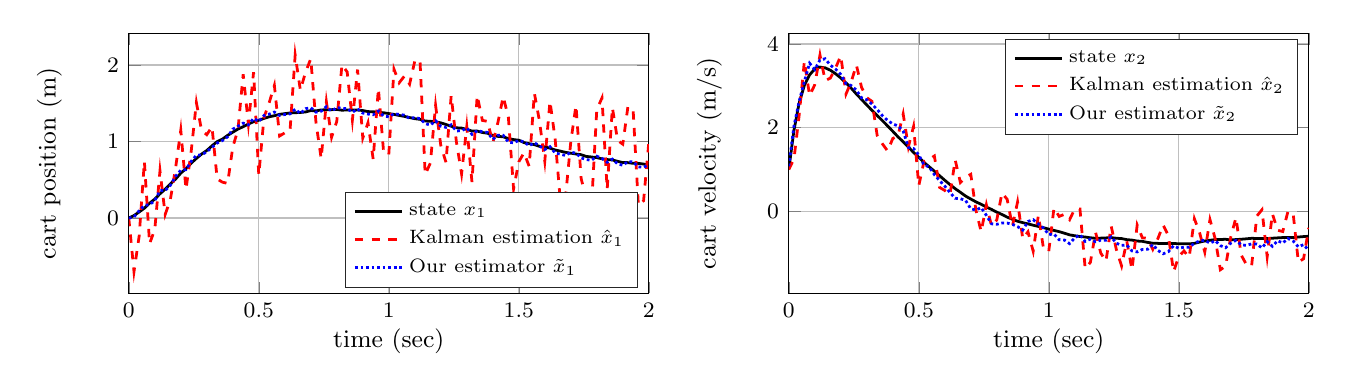
\begin{tikzpicture}
\begin{axis}
[	width=2.6in,
	height=1.3in,
	at={(0in,1.7in)},
	scale only axis,
	xmin=0,
	xmax=2.0,
	xlabel={\small time (sec)},
	ylabel={\small cart position (m)},
	x label style={at={(axis description cs:0.5,-0.1)},anchor=north},
	y label style={at={(axis description cs:-0.11,.5)},anchor=south},
	xticklabel style = {font=\footnotesize},
	yticklabel style = {font=\footnotesize},
	axis background/.style={fill=white},
	xmajorgrids,
	ymajorgrids,
	legend style={at={(0.98,0.02)}, anchor=south east, legend cell align=left, align=left, draw=white!15!black, font=\scriptsize}]
	 \addplot [color={black}, line width=1pt]
	table[row sep={\\}]
	{
0.0  0.0  \\
0.02  0.0312885282018752  \\
0.04  0.0788123875203588  \\
0.06  0.12783983276693056  \\
0.08  0.19302443002512482  \\
0.1  0.24691171369130704  \\
0.12  0.3161471924463811  \\
0.14  0.37655820357754827  \\
0.16  0.44574118653184464  \\
0.18  0.508717686134174  \\
0.2  0.5858944594685165  \\
0.22  0.6442080290694358  \\
0.24  0.7170003106288797  \\
0.26  0.7781390817476541  \\
0.28  0.8348607428170365  \\
0.3  0.8820850124163883  \\
0.32  0.9429843329186438  \\
0.34  0.9985281560618742  \\
0.36  1.0302635273555911  \\
0.38  1.0791321889652439  \\
0.4  1.121245022981027  \\
0.42  1.161891300602804  \\
0.44  1.192700117051156  \\
0.46  1.2287933108791957  \\
0.48  1.2579103583060975  \\
0.5  1.2769090558718827  \\
0.52  1.3010074939994656  \\
0.54  1.322606952127935  \\
0.56  1.3363739300408208  \\
0.58  1.3547060181087645  \\
0.6  1.3637156124358794  \\
0.62  1.372208147950066  \\
0.64  1.3758158415504202  \\
0.66  1.3789775570173455  \\
0.68  1.3858658992171147  \\
0.7  1.4038540774769968  \\
0.72  1.399388270372787  \\
0.74  1.4121158471937587  \\
0.76  1.413967536880243  \\
0.78  1.4159014376757404  \\
0.8  1.417828678620937  \\
0.82  1.408439121962671  \\
0.84  1.4119812043541529  \\
0.86  1.4115583441626582  \\
0.88  1.4107211138008886  \\
0.9  1.4043543531943106  \\
0.92  1.390269579268504  \\
0.94  1.388444098074998  \\
0.96  1.3811571553361286  \\
0.98  1.375136659753237  \\
1.0  1.3650405410205926  \\
1.02  1.3532746327113854  \\
1.04  1.3399687394128827  \\
1.06  1.3274222529638806  \\
1.08  1.312887237057181  \\
1.1  1.297953855938006  \\
1.12  1.2888243656725031  \\
1.14  1.2671580891040044  \\
1.16  1.2636596712198738  \\
1.18  1.2568123705161265  \\
1.2  1.2433534208208616  \\
1.22  1.222018058868546  \\
1.24  1.199082947901861  \\
1.26  1.1789132315105741  \\
1.28  1.1746923163614416  \\
1.3  1.1574829037716936  \\
1.32  1.1356654326585793  \\
1.34  1.1362230591177622  \\
1.36  1.1171876047888512  \\
1.38  1.1074990138885137  \\
1.4  1.078974551777622  \\
1.42  1.0661973181301283  \\
1.44  1.0609127088404313  \\
1.46  1.0372993334160026  \\
1.48  1.024440355201395  \\
1.5  1.016773165435164  \\
1.52  0.985372726177421  \\
1.54  0.9708403750356196  \\
1.56  0.9591509832628655  \\
1.58  0.9355856912687716  \\
1.6  0.9288408011304456  \\
1.62  0.9124527452153604  \\
1.64  0.888692309701688  \\
1.66  0.8736279796836832  \\
1.68  0.8576149131794482  \\
1.7  0.8467338065845937  \\
1.72  0.8357323419078908  \\
1.74  0.8271295129691318  \\
1.76  0.804168519172342  \\
1.78  0.7973787024419723  \\
1.8  0.7885831880803513  \\
1.82  0.7731913576797228  \\
1.84  0.7632841476573989  \\
1.86  0.7581919965043644  \\
1.88  0.7404424073275442  \\
1.9  0.7242330930938433  \\
1.92  0.7232652267292055  \\
1.94  0.7141451711559598  \\
1.96  0.7135626060421556  \\
1.98  0.7050839449630739  \\
2.0  0.6894219585423397  \\
	}
	;\addlegendentry{state $x_1$}
	
	\addplot [color={red},dashed, line width=1pt]
	table[row sep={\\}]
	{
 0.0  0.0  \\
0.02  -0.7016326820685982  \\
0.04  -0.23585571586261345  \\
0.06  0.7396609099297807  \\
0.08  -0.33621243440965815  \\
0.1  -0.15048791253219151  \\
0.12  0.6176826620511138  \\
0.14  0.04578213612712215  \\
0.16  0.24085153712000212  \\
0.18  0.6519749416537854  \\
0.2  1.1481340088757428  \\
0.22  0.3739654072288668  \\
0.24  0.8695195317551777  \\
0.26  1.5079986424406817  \\
0.28  1.1437489242746022  \\
0.3  1.0884297575593251  \\
0.32  1.192645206389877  \\
0.34  0.5096949773855692  \\
0.36  0.4682016134464051  \\
0.38  0.45158731684792996  \\
0.4  0.9245292733660191  \\
0.42  1.1563184823107087  \\
0.44  1.8782643853325425  \\
0.46  1.2286200415610418  \\
0.48  1.90560288844914  \\
0.5  0.5609048675886162  \\
0.52  1.314072432246385  \\
0.54  1.506294966924829  \\
0.56  1.732157136746129  \\
0.58  1.0713638460394828  \\
0.6  1.1124754014038012  \\
0.62  1.1325698189447386  \\
0.64  2.1299447613993494  \\
0.66  1.6694764974183034  \\
0.68  1.9074552913612985  \\
0.7  2.0802230570514464  \\
0.72  1.249075947340938  \\
0.74  0.7755524566336746  \\
0.76  1.5186582695973136  \\
0.78  1.053934096560571  \\
0.8  1.263845037327248  \\
0.82  2.004341804511319  \\
0.84  1.9076177543863433  \\
0.86  1.2791803217886837  \\
0.88  1.9388924541370987  \\
0.9  1.044856742034207  \\
0.92  1.2434718255294455  \\
0.94  0.7678933158489609  \\
0.96  1.6943045521016002  \\
0.98  0.8649726988503483  \\
1.0  0.826956736056349  \\
1.02  1.9441067890112704  \\
1.04  1.7671483990223398  \\
1.06  1.8537757329684719  \\
1.08  1.74869596272442  \\
1.1  2.050331385127062  \\
1.12  2.065323459242827  \\
1.14  0.5675645417737036  \\
1.16  0.7183137980272856  \\
1.18  1.4721749444770658  \\
1.2  0.9486696263681218  \\
1.22  0.7275878036994118  \\
1.24  1.5982571538598647  \\
1.26  0.9968108122528502  \\
1.28  0.5771790217717717  \\
1.3  1.1939220530371921  \\
1.32  0.4705513491038608  \\
1.34  1.6017654267607948  \\
1.36  1.2754776607476657  \\
1.38  1.2618686905389338  \\
1.4  0.9821092898946824  \\
1.42  1.2520370722954877  \\
1.44  1.5868463335267238  \\
1.46  1.315316213744334  \\
1.48  0.3809467176356255  \\
1.5  0.7343497684517054  \\
1.52  0.8525011066231617  \\
1.54  0.6747786775563649  \\
1.56  1.631306074588672  \\
1.58  1.259238093266994  \\
1.6  0.7406502576917274  \\
1.62  1.5270858735962223  \\
1.64  1.0273604220689518  \\
1.66  0.22013248694006454  \\
1.68  0.2814102904932267  \\
1.7  0.9937623709318437  \\
1.72  1.4722659204159319  \\
1.74  0.513230720725658  \\
1.76  0.24399096723995706  \\
1.78  0.17209686923052656  \\
1.8  1.414894962085707  \\
1.82  1.5689427180553022  \\
1.84  0.3738299073894682  \\
1.86  1.4432830585706296  \\
1.88  1.0146304626081781  \\
1.9  0.9646143450049791  \\
1.92  1.4599263074280486  \\
1.94  1.3992941378715475  \\
1.96  0.16577497949085318  \\
1.98  0.2250988953546872  \\
2.0  0.9813678260080361  \\
	}
	;\addlegendentry{{ Kalman estimation $\hat{x}_1$}}
    \addplot[densely dotted, color={blue}, line width=1pt]
        table[row sep={\\}]
        {
  0.0  -0.0016546478915138397  \\
0.02  0.012803800843751626  \\
0.04  0.09554688470489497  \\
0.06  0.16253616814154492  \\
0.08  0.1757155439630189  \\
0.1  0.22684144474391166  \\
0.12  0.3588610317373191  \\
0.14  0.3600565285670698  \\
0.16  0.4268314405275966  \\
0.18  0.5444687411092691  \\
0.2  0.6240844791843322  \\
0.22  0.6314795408897524  \\
0.24  0.7400311038559425  \\
0.26  0.8189832083536872  \\
0.28  0.8244024397244267  \\
0.3  0.8663905052304092  \\
0.32  0.922990301770209  \\
0.34  0.9798892619734936  \\
0.36  1.0117967230429303  \\
0.38  1.0599172908675325  \\
0.4  1.1603643852567949  \\
0.42  1.1990802015445396  \\
0.44  1.2395813207698205  \\
0.46  1.2165585171583397  \\
0.48  1.3013264919921557  \\
0.5  1.2609307571835484  \\
0.52  1.3386884784369582  \\
0.54  1.357083577925525  \\
0.56  1.3842326654411976  \\
0.58  1.3398267024517447  \\
0.6  1.3518845191939897  \\
0.62  1.3605004189076775  \\
0.64  1.4219380480003003  \\
0.66  1.3649203285273799  \\
0.68  1.4285890406210218  \\
0.7  1.4410836824050024  \\
0.72  1.3826840414912316  \\
0.74  1.3959236008102323  \\
0.76  1.4552823453620856  \\
0.78  1.3959039513270748  \\
0.8  1.4438071511837156  \\
0.82  1.432844078488602  \\
0.84  1.4299867320429205  \\
0.86  1.3813759762529558  \\
0.88  1.4265818351347233  \\
0.9  1.3709250480900586  \\
0.92  1.3579677545976403  \\
0.94  1.3487742263587437  \\
0.96  1.3975588490058366  \\
0.98  1.33454216140927  \\
1.0  1.3216205976334596  \\
1.02  1.3624960268492265  \\
1.04  1.353311126347017  \\
1.06  1.3439501738480442  \\
1.08  1.301369848305021  \\
1.1  1.3125870668179422  \\
1.12  1.2980724796332295  \\
1.14  1.2338677686687103  \\
1.16  1.2137553744273737  \\
1.18  1.2709021953976292  \\
1.2  1.1992025218793143  \\
1.22  1.183697398088326  \\
1.24  1.218570516572107  \\
1.26  1.137563007619231  \\
1.28  1.1405022675978889  \\
1.3  1.1765535132579692  \\
1.32  1.0928758663920797  \\
1.34  1.1414652285997844  \\
1.36  1.1271940964802922  \\
1.38  1.1178376669643972  \\
1.4  1.0277986083364172  \\
1.42  1.0805816091531892  \\
1.44  1.0807849167204544  \\
1.46  0.9920763178114405  \\
1.48  0.9817306703518764  \\
1.5  1.0134477693156418  \\
1.52  0.9951974251474277  \\
1.54  0.9442285914088713  \\
1.56  0.9833197436088972  \\
1.58  0.9409151710618642  \\
1.6  0.8946300833123895  \\
1.62  0.9316112622492073  \\
1.64  0.8489701821077618  \\
1.66  0.8339106994871763  \\
1.68  0.8161789446932478  \\
1.7  0.859266662119662  \\
1.72  0.8476876655078228  \\
1.74  0.7855933449829767  \\
1.76  0.7624117087703305  \\
1.78  0.7551194589099179  \\
1.8  0.8077894968082772  \\
1.82  0.7782348664563057  \\
1.84  0.7291031405864548  \\
1.86  0.7692963458943343  \\
1.88  0.7074919875254148  \\
1.9  0.6891930843264874  \\
1.92  0.7372792789114803  \\
1.94  0.7335083478070233  \\
1.96  0.668317016120237  \\
1.98  0.6637710011872  \\
2.0  0.6980071501144504  \\
        }
        ;\addlegendentry{{ Our estimator $\tilde{x}_1$}}
        
\end{axis}

\begin{axis}
[	width=2.6in,
height=1.3in,
at={(3.3in,1.7in)},
scale only axis,
xmin=0,
xmax=2.0,
xlabel={\small time (sec)},
ylabel={\small cart velocity (m/s)},
x label style={at={(axis description cs:0.5,-0.1)},anchor=north},
y label style={at={(axis description cs:-0.11,.5)},anchor=south},
xticklabel style = {font=\footnotesize},
yticklabel style = {font=\footnotesize},
axis background/.style={fill=white},
xmajorgrids,
ymajorgrids,
legend style={at={(0.98,0.98)}, anchor=north east, legend cell align=left, align=left, draw=white!15!black, font=\scriptsize}]
\addplot [color={black}, line width=1pt]
table[row sep={\\}]
{
0.0  1.0  \\
0.02  1.9391209237895848  \\
0.04  2.590989465213296  \\
0.06  3.0112038136322097  \\
0.08  3.262145933341507  \\
0.1  3.404055223712122  \\
0.12  3.448329465319425  \\
0.14  3.4304868325634814  \\
0.16  3.372844199991032  \\
0.18  3.289148790648013  \\
0.2  3.1885535486300065  \\
0.22  3.0692926604120068  \\
0.24  2.944939735179303  \\
0.26  2.8041012335303797  \\
0.28  2.6741250131880947  \\
0.3  2.542186317426113  \\
0.32  2.4133137843864088  \\
0.34  2.2902036362827154  \\
0.36  2.1676068541377513  \\
0.38  2.041575453393154  \\
0.4  1.912003547154351  \\
0.42  1.7805111075137916  \\
0.44  1.6613280032011057  \\
0.46  1.5367336043391617  \\
0.48  1.4056656658012763  \\
0.5  1.290973151946963  \\
0.52  1.1679927469559728  \\
0.54  1.0638319121527307  \\
0.56  0.9574423074532515  \\
0.58  0.8490799761838703  \\
0.6  0.7412336946439754  \\
0.62  0.6375781972725671  \\
0.64  0.5397855090185257  \\
0.66  0.4532142587467182  \\
0.68  0.36280368622739734  \\
0.7  0.2917937269950741  \\
0.72  0.22364279659665026  \\
0.74  0.16641956056250445  \\
0.76  0.09957734983786248  \\
0.78  0.04285943612658093  \\
0.8  -0.021996866697433476  \\
0.82  -0.07785062469992182  \\
0.84  -0.14179940204160668  \\
0.86  -0.192111834507433  \\
0.88  -0.2395799342971533  \\
0.9  -0.2731098299450826  \\
0.92  -0.3023493674467045  \\
0.94  -0.33494599088485866  \\
0.96  -0.3634837919419665  \\
0.98  -0.39429252436904916  \\
1.0  -0.427376069393288  \\
1.02  -0.45849247351460987  \\
1.04  -0.4886944820743368  \\
1.06  -0.5253851993311534  \\
1.08  -0.5650389302187308  \\
1.1  -0.5863884385696589  \\
1.12  -0.6038458947549443  \\
1.14  -0.6171167795918366  \\
1.16  -0.6349431570995152  \\
1.18  -0.6474517267585185  \\
1.2  -0.6434772685824866  \\
1.22  -0.6379941265376432  \\
1.24  -0.6322982024232  \\
1.26  -0.6458598128233805  \\
1.28  -0.654065958989119  \\
1.3  -0.679509056048515  \\
1.32  -0.6905768067028223  \\
1.34  -0.7130004889104322  \\
1.36  -0.7203615215047533  \\
1.38  -0.7454102026881453  \\
1.4  -0.7645886120566366  \\
1.42  -0.7688770436773459  \\
1.44  -0.7733996969520899  \\
1.46  -0.767714095270773  \\
1.48  -0.7704943594144114  \\
1.5  -0.7792436303557043  \\
1.52  -0.7763125311369948  \\
1.54  -0.7800818638691298  \\
1.56  -0.7683618200545922  \\
1.58  -0.7379645382430333  \\
1.6  -0.7120211968404369  \\
1.62  -0.6944313784107807  \\
1.64  -0.6788356905664363  \\
1.66  -0.6755209780869861  \\
1.68  -0.6713863855448137  \\
1.7  -0.6861143109771883  \\
1.72  -0.6777605242430396  \\
1.74  -0.67008745456601  \\
1.76  -0.6595296803854034  \\
1.78  -0.6480090140165278  \\
1.8  -0.651450136105128  \\
1.82  -0.6517143018493359  \\
1.84  -0.6525749963680775  \\
1.86  -0.6453041999310413  \\
1.88  -0.6373422062650471  \\
1.9  -0.630057062238385  \\
1.92  -0.6301433102561566  \\
1.94  -0.6297353309511714  \\
1.96  -0.616497720752044  \\
1.98  -0.6064299270620612  \\
2.0  -0.5981417131472986  \\
}
;\addlegendentry{state $x_2$}

\addplot [color={red},dashed, line width=1pt]
table[row sep={\\}]
{
   0.0  1.0  \\
0.02  1.2520375776998334  \\
0.04  2.300009604013391  \\
0.06  3.592060558953479  \\
0.08  2.7649250252416024  \\
0.1  3.0262809894865192  \\
0.12  3.737499294098212  \\
0.14  3.12110372825729  \\
0.16  3.1861891324106963  \\
0.18  3.4274138963467804  \\
0.2  3.7198764070873898  \\
0.22  2.803236665480386  \\
0.24  3.0913857467081614  \\
0.26  3.500316410919404  \\
0.28  2.961819884446753  \\
0.3  2.7158798761007077  \\
0.32  2.628985356939085  \\
0.34  1.812881338210877  \\
0.36  1.613351795096433  \\
0.38  1.4425020734693912  \\
0.4  1.7399265201110468  \\
0.42  1.8028149398680218  \\
0.44  2.326401112633281  \\
0.46  1.5423332185675656  \\
0.48  2.0287784649248946  \\
0.5  0.6102389896017371  \\
0.52  1.191268735603829  \\
0.54  1.237764042431899  \\
0.56  1.3224531999777234  \\
0.58  0.5704468281498346  \\
0.6  0.49673279383399516  \\
0.62  0.3981857887619049  \\
0.64  1.229096741477517  \\
0.66  0.6877935606365496  \\
0.68  0.8141279419565274  \\
0.7  0.8835958773833297  \\
0.72  0.020568475438498934  \\
0.74  -0.48943871844095244  \\
0.76  0.15514500137660914  \\
0.78  -0.35244027450211646  \\
0.8  -0.20815875770989178  \\
0.82  0.438027801028096  \\
0.84  0.2843113304577627  \\
0.86  -0.36055354865939027  \\
0.88  0.22295697043163942  \\
0.9  -0.6589673240118565  \\
0.92  -0.49078963983506707  \\
0.94  -0.9568518427371487  \\
0.96  -0.09412376172945769  \\
0.98  -0.9039459953155622  \\
1.0  -0.9563233110889232  \\
1.02  0.07966430313712625  \\
1.04  -0.12380509206160606  \\
1.06  -0.07402619999655324  \\
1.08  -0.2030130407085846  \\
1.1  0.056772989288457865  \\
1.12  0.052243394850999936  \\
1.14  -1.3723270099750198  \\
1.16  -1.223561027584351  \\
1.18  -0.5057712567390962  \\
1.2  -1.0011869394094126  \\
1.22  -1.1949065410616595  \\
1.24  -0.3549026777961153  \\
1.26  -0.9183435604352458  \\
1.28  -1.3080548317301632  \\
1.3  -0.7141746173316741  \\
1.32  -1.40188819595665  \\
1.34  -0.32959480344887826  \\
1.36  -0.6367413723090429  \\
1.38  -0.6468663524250073  \\
1.4  -0.9123046246791389  \\
1.42  -0.6493285146517109  \\
1.44  -0.3288712775744558  \\
1.46  -0.5838383248759282  \\
1.48  -1.4457255354947045  \\
1.5  -1.081487548739723  \\
1.52  -0.9510426624820778  \\
1.54  -1.1035250307171802  \\
1.56  -0.17920451360073142  \\
1.58  -0.5104956175392936  \\
1.6  -0.9774753425770938  \\
1.62  -0.20198433902106339  \\
1.64  -0.6568916513437502  \\
1.66  -1.400750886670715  \\
1.68  -1.3131253278757518  \\
1.7  -0.615670432340711  \\
1.72  -0.15068321641309024  \\
1.74  -1.046636962700916  \\
1.76  -1.2754309384409042  \\
1.78  -1.3185154829093082  \\
1.8  -0.11618707527794592  \\
1.82  0.03486447792739433  \\
1.84  -1.0885087582132544  \\
1.86  -0.05963010563322024  \\
1.88  -0.4554360354252778  \\
1.9  -0.48533050983918957  \\
1.92  -0.004104539990258171  \\
1.94  -0.05907869157379575  \\
1.96  -1.2193817306049763  \\
1.98  -1.1368577322583464  \\
2.0  -0.39764266241265944  \\
}
;\addlegendentry{{ Kalman estimation $\hat{x}_2$}}
\addplot[densely dotted, color={blue}, line width=1pt]
table[row sep={\\}]
{
 0.0  1.0766943557990734  \\
0.02  2.0402360299618394  \\
0.04  2.6309454758292494  \\
0.06  3.1068675196902764  \\
0.08  3.54080134552669  \\
0.1  3.390423831584909  \\
0.12  3.6176773435075993  \\
0.14  3.6483302835825806  \\
0.16  3.4940837403221066  \\
0.18  3.400518174132703  \\
0.2  3.272179041445286  \\
0.22  3.051182580312056  \\
0.24  3.007136640276949  \\
0.26  2.89668735820574  \\
0.28  2.713233393415006  \\
0.3  2.666081620611238  \\
0.32  2.562083551484879  \\
0.34  2.434075387513464  \\
0.36  2.286871848307895  \\
0.38  2.1725112918581857  \\
0.4  2.0891911107037067  \\
0.42  2.0406855463131692  \\
0.44  1.9222977654197195  \\
0.46  1.5257739757194784  \\
0.48  1.4989888926426562  \\
0.5  1.3473304530955497  \\
0.52  1.109572133570126  \\
0.54  1.0592201977960447  \\
0.56  0.8758454837144379  \\
0.58  0.7337559238480325  \\
0.6  0.6004573856743581  \\
0.62  0.44824465603343244  \\
0.64  0.3101689801671155  \\
0.66  0.2987946638154928  \\
0.68  0.2600433017728896  \\
0.7  0.05672463712827543  \\
0.72  0.030413094277216744  \\
0.74  0.08555028416184272  \\
0.76  -0.09971583953501285  \\
0.78  -0.3017142438245463  \\
0.8  -0.3122042796770449  \\
0.82  -0.2827534315188673  \\
0.84  -0.2829505347667381  \\
0.86  -0.31444525280989494  \\
0.88  -0.3679083896574561  \\
0.9  -0.4523096410930004  \\
0.92  -0.24528076875533894  \\
0.94  -0.2012204257573242  \\
0.96  -0.30459353150941115  \\
0.98  -0.4034606060932498  \\
1.0  -0.5579468081734421  \\
1.02  -0.5456885041145905  \\
1.04  -0.6834788869342028  \\
1.06  -0.6876029558751029  \\
1.08  -0.7754242277751354  \\
1.1  -0.6357568393571198  \\
1.12  -0.5647630895137999  \\
1.14  -0.722224950479285  \\
1.16  -0.6672023210232  \\
1.18  -0.730160044324085  \\
1.2  -0.6932767721446531  \\
1.22  -0.6955416637290003  \\
1.24  -0.6148744413228993  \\
1.26  -0.7646738905171426  \\
1.28  -0.8174879195874942  \\
1.3  -0.8086440314412106  \\
1.32  -0.9489524673668117  \\
1.34  -0.9731834368682155  \\
1.36  -0.9134270631253525  \\
1.38  -0.9095082237264895  \\
1.4  -0.7968292615369957  \\
1.42  -0.9388984989978707  \\
1.44  -1.0175358467975835  \\
1.46  -0.9680022103203125  \\
1.48  -0.8260065615129651  \\
1.5  -0.886260333768104  \\
1.52  -0.8603670806734103  \\
1.54  -0.8640190493688218  \\
1.56  -0.7640364116753472  \\
1.58  -0.7120111509452782  \\
1.6  -0.6936300126424111  \\
1.62  -0.764741414382075  \\
1.64  -0.7033854196176764  \\
1.66  -0.8226871876980503  \\
1.68  -0.8731757555208807  \\
1.7  -0.7626857480875107  \\
1.72  -0.6967479415177407  \\
1.74  -0.8031387793448946  \\
1.76  -0.8170700823758712  \\
1.78  -0.7816777307010934  \\
1.8  -0.7845261659077962  \\
1.82  -0.8770371475311388  \\
1.84  -0.7264585052225073  \\
1.86  -0.8394900475907195  \\
1.88  -0.705278834141262  \\
1.9  -0.760571799602993  \\
1.92  -0.650966035713089  \\
1.94  -0.7135157071013508  \\
1.96  -0.8527263663135067  \\
1.98  -0.7989930114769055  \\
2.0  -0.9373767100494399  \\
}
;\addlegendentry{{ Our estimator $\tilde{x}_2$}}

\end{axis}

%  	\begin{axis}
%	[	width=2.6in,
%	height=1.3in,
%	at={(0in,0in)},
%	scale only axis,
%	xmin=0,
%	xmax=2.0,
%%	ymin=-4,
%%	ymax=2,
%	xlabel={\small time (sec)},
%	ylabel={\small $x_3$ pendulumn angle},
%	x label style={at={(axis description cs:0.5,-0.1)},anchor=north},
%	y label style={at={(axis description cs:-0.11,.5)},anchor=south},
%	xticklabel style = {font=\footnotesize},
%	yticklabel style = {font=\footnotesize},
%	axis background/.style={fill=white},
%	xmajorgrids,
%	ymajorgrids,
%	legend style={at={(0.98,0.02)}, anchor=south east, legend cell align=left, align=left, draw=white!15!black, font=\scriptsize}]
%	\addplot [color={black}, line width=1pt]
%	table[row sep={\\}]
%	{
%0.0  0.0  \\
%0.02  0.00772853593415913  \\
%0.04  0.004801671416923327  \\
%0.06  -0.012528997431996048  \\
%0.08  -0.034478619332425936  \\
%0.1  -0.06220231524500317  \\
%0.12  -0.08812635048651297  \\
%0.14  -0.11408845091735348  \\
%0.16  -0.14488997218330013  \\
%0.18  -0.16947348245078697  \\
%0.2  -0.19501471373927462  \\
%0.22  -0.2166030568036244  \\
%0.24  -0.23694887645664164  \\
%0.26  -0.2534179553657174  \\
%0.28  -0.2659048131170473  \\
%0.3  -0.2814074322954603  \\
%0.32  -0.2947651384686937  \\
%0.34  -0.30280625979339526  \\
%0.36  -0.3110461733895194  \\
%0.38  -0.322599925444607  \\
%0.4  -0.3266601375700984  \\
%0.42  -0.32832183302190043  \\
%0.44  -0.33079378651792585  \\
%0.46  -0.33139999061403563  \\
%0.48  -0.33190912976035625  \\
%0.5  -0.32830514918189446  \\
%0.52  -0.3265624628054656  \\
%0.54  -0.3231032971609128  \\
%0.56  -0.31943423376946206  \\
%0.58  -0.31567219360956844  \\
%0.6  -0.3139459878003922  \\
%0.62  -0.30858429971742735  \\
%0.64  -0.302866065490615  \\
%0.66  -0.2975240107704187  \\
%0.68  -0.29156813130488785  \\
%0.7  -0.28705864201984305  \\
%0.72  -0.2800613967051828  \\
%0.74  -0.2721345042496352  \\
%0.76  -0.2675647476463787  \\
%0.78  -0.26004373544306775  \\
%0.8  -0.24895562242482422  \\
%0.82  -0.24469615255703123  \\
%0.84  -0.23679296240647962  \\
%0.86  -0.22526462977535064  \\
%0.88  -0.21530137387528134  \\
%0.9  -0.2019610820610649  \\
%0.92  -0.19283115640996426  \\
%0.94  -0.18404650174938508  \\
%0.96  -0.1761938176509628  \\
%0.98  -0.16952154188571567  \\
%1.0  -0.16068318494400077  \\
%1.02  -0.15115385465801076  \\
%1.04  -0.142077499764086  \\
%1.06  -0.13285231555738442  \\
%1.08  -0.12217488148841449  \\
%1.1  -0.11717625074624005  \\
%1.12  -0.11014342489808715  \\
%1.14  -0.10290962697247244  \\
%1.16  -0.09707223606283309  \\
%1.18  -0.08535583686102192  \\
%1.2  -0.07985586728850495  \\
%1.22  -0.07053290137389215  \\
%1.24  -0.0660756875734225  \\
%1.26  -0.05925950423578198  \\
%1.28  -0.04983238664926049  \\
%1.3  -0.046321730532286276  \\
%1.32  -0.04111947230774583  \\
%1.34  -0.03716014124124552  \\
%1.36  -0.026958173254637667  \\
%1.38  -0.02105479624823502  \\
%1.4  -0.013204082238369545  \\
%1.42  -0.007208612852129617  \\
%1.44  -0.005029793064317797  \\
%1.46  -0.0030365387904538444  \\
%1.48  -0.004685191023569348  \\
%1.5  -0.0013502134977833556  \\
%1.52  -0.0012637857934116841  \\
%1.54  -0.0012840803221537893  \\
%1.56  0.004161592495718868  \\
%1.58  0.007337270321035059  \\
%1.6  0.007873265952081725  \\
%1.62  0.007756595504494869  \\
%1.64  0.012948213825993315  \\
%1.66  0.01713997304166258  \\
%1.68  0.019303428528959714  \\
%1.7  0.021720664071569973  \\
%1.72  0.021496525088056485  \\
%1.74  0.02269954427453162  \\
%1.76  0.025127263635035712  \\
%1.78  0.025581388241573386  \\
%1.8  0.022956371536018347  \\
%1.82  0.020320909246699284  \\
%1.84  0.02325727363447171  \\
%1.86  0.022566429135964905  \\
%1.88  0.025410932971556357  \\
%1.9  0.025581397517493814  \\
%1.92  0.024133015365711413  \\
%1.94  0.024607306183292644  \\
%1.96  0.02686997993370564  \\
%1.98  0.028618584557972122  \\
%2.0  0.02949612536857937  \\
%	}
%	;\addlegendentry{state $x_3$}
%	\addplot [color={red},dashed, line width=1pt]
%	table[row sep={\\}]
%	{
%	 0.0  0.0  \\
%	0.02  0.00809402453328914  \\
%	0.04  0.002283710058266839  \\
%	0.06  -0.011924222353404363  \\
%	0.08  -0.03538807548199385  \\
%	0.1  -0.062495688561897404  \\
%	0.12  -0.08979727756857352  \\
%	0.14  -0.11596912737252132  \\
%	0.16  -0.14427298978459968  \\
%	0.18  -0.1699091880689923  \\
%	0.2  -0.19571409358693093  \\
%	0.22  -0.21710723871475957  \\
%	0.24  -0.23750518798723996  \\
%	0.26  -0.2523487237267693  \\
%	0.28  -0.26564551359739796  \\
%	0.3  -0.28113924184632594  \\
%	0.32  -0.29344313265186917  \\
%	0.34  -0.30387742299429843  \\
%	0.36  -0.31093266172634626  \\
%	0.38  -0.32032314034771303  \\
%	0.4  -0.32488432492231156  \\
%	0.42  -0.328256133800731  \\
%	0.44  -0.33170684466667966  \\
%	0.46  -0.33284554813223155  \\
%	0.48  -0.32934060251669267  \\
%	0.5  -0.32881415681358606  \\
%	0.52  -0.32672393145274836  \\
%	0.54  -0.3217023284966502  \\
%	0.56  -0.31920782046530927  \\
%	0.58  -0.3155857583713461  \\
%	0.6  -0.31200171978648444  \\
%	0.62  -0.30753884981430435  \\
%	0.64  -0.30328744734313084  \\
%	0.66  -0.298819639225292  \\
%	0.68  -0.2916263924411364  \\
%	0.7  -0.2838538399639527  \\
%	0.72  -0.27822533107121034  \\
%	0.74  -0.27214850374295424  \\
%	0.76  -0.2649862125224101  \\
%	0.78  -0.2581935349054245  \\
%	0.8  -0.24687375692743166  \\
%	0.82  -0.24215334598492766  \\
%	0.84  -0.23463968652823464  \\
%	0.86  -0.2266454648618093  \\
%	0.88  -0.21570653361944153  \\
%	0.9  -0.20378113555698663  \\
%	0.92  -0.1922094272504351  \\
%	0.94  -0.18193892229656553  \\
%	0.96  -0.17462306148804935  \\
%	0.98  -0.16857998362472904  \\
%	1.0  -0.1589098101915298  \\
%	1.02  -0.1502282447377052  \\
%	1.04  -0.14310208638808308  \\
%	1.06  -0.13391428982914821  \\
%	1.08  -0.12206666034954945  \\
%	1.1  -0.11753381580332939  \\
%	1.12  -0.11064111898353321  \\
%	1.14  -0.10215982660161821  \\
%	1.16  -0.096618902112179  \\
%	1.18  -0.08817640412095815  \\
%	1.2  -0.07931844432254224  \\
%	1.22  -0.0713170158403937  \\
%	1.24  -0.06598326032462205  \\
%	1.26  -0.05869782541506201  \\
%	1.28  -0.05244831403760163  \\
%	1.3  -0.04689123976106053  \\
%	1.32  -0.04325454089798624  \\
%	1.34  -0.03885220256504527  \\
%	1.36  -0.030517495413270805  \\
%	1.38  -0.024466342268987945  \\
%	1.4  -0.018729185184462  \\
%	1.42  -0.010157661361933055  \\
%	1.44  -0.005799650225733364  \\
%	1.46  -0.0017710381011364653  \\
%	1.48  -0.002224799382994183  \\
%	1.5  -0.0037629560253844437  \\
%	1.52  -0.00020440203585928116  \\
%	1.54  0.0012643359647233753  \\
%	1.56  0.003252784378121404  \\
%	1.58  0.005266412443152401  \\
%	1.6  0.006949937595322902  \\
%	1.62  0.008256452575278935  \\
%	1.64  0.012007453507124496  \\
%	1.66  0.01615310418726861  \\
%	1.68  0.019000666804788804  \\
%	1.7  0.022087371511188413  \\
%	1.72  0.022261092399250972  \\
%	1.74  0.02355749395802008  \\
%	1.76  0.023895346270558754  \\
%	1.78  0.026333022304786253  \\
%	1.8  0.02456626556539792  \\
%	1.82  0.021605386228436392  \\
%	1.84  0.023528349423668403  \\
%	1.86  0.023572743261476937  \\
%	1.88  0.025126899283551846  \\
%	1.9  0.025833933274513415  \\
%	1.92  0.02280935517999988  \\
%	1.94  0.025189469054832925  \\
%	1.96  0.02661138935665535  \\
%	1.98  0.02763011362829756  \\
%	2.0  0.027469141828147026  \\
%	}
%	;\addlegendentry{{ Kalman estimation $\hat{x}_3$}}
%	\addplot[densely dotted, color={blue}, line width=1pt]
%	table[row sep={\\}]
%	{
%    0.0  1.8153964737662312e-5  \\
%0.02  0.0066894619554046355  \\
%0.04  0.0018375871994040162  \\
%0.06  -0.011012697570773474  \\
%0.08  -0.03609804873935931  \\
%0.1  -0.06340645502442915  \\
%0.12  -0.0895457918792631  \\
%0.14  -0.11546107462068377  \\
%0.16  -0.14461477831571443  \\
%0.18  -0.17007154514361927  \\
%0.2  -0.1965051643232883  \\
%0.22  -0.2166340902306285  \\
%0.24  -0.23770039325448397  \\
%0.26  -0.2507335125541037  \\
%0.28  -0.2645156857629006  \\
%0.3  -0.28216527675191616  \\
%0.32  -0.2939902057265568  \\
%0.34  -0.30440857374041375  \\
%0.36  -0.31047444062583235  \\
%0.38  -0.32198495278139255  \\
%0.4  -0.3249118700086211  \\
%0.42  -0.32841640163734204  \\
%0.44  -0.33251010788936297  \\
%0.46  -0.3331188005365526  \\
%0.48  -0.32767165979082796  \\
%0.5  -0.3288637216034393  \\
%0.52  -0.3265504673964966  \\
%0.54  -0.3205275268798475  \\
%0.56  -0.3197884422608594  \\
%0.58  -0.3157679939079811  \\
%0.6  -0.31254421435944685  \\
%0.62  -0.30806083114358135  \\
%0.64  -0.3038352148338218  \\
%0.66  -0.2994116819525727  \\
%0.68  -0.29121889287466646  \\
%0.7  -0.2833617882231757  \\
%0.72  -0.27936861590095097  \\
%0.74  -0.27290542088826425  \\
%0.76  -0.2654318394097727  \\
%0.78  -0.25942935600796185  \\
%0.8  -0.2457658293296008  \\
%0.82  -0.24403414344605018  \\
%0.84  -0.2358616914531913  \\
%0.86  -0.2275077308550984  \\
%0.88  -0.21485981313066116  \\
%0.9  -0.20232178782749977  \\
%0.92  -0.19104608352709898  \\
%0.94  -0.18111885006671183  \\
%0.96  -0.1754534261052666  \\
%0.98  -0.17003134488456753  \\
%1.0  -0.15878283143959224  \\
%1.02  -0.15051065091807594  \\
%1.04  -0.1435009071579159  \\
%1.06  -0.13363074186982313  \\
%1.08  -0.12038778178826819  \\
%1.1  -0.11866338138681089  \\
%1.12  -0.110930248968576  \\
%1.14  -0.10181163345285733  \\
%1.16  -0.09751700179946482  \\
%1.18  -0.08758702035485068  \\
%1.2  -0.07785509840417323  \\
%1.22  -0.07050311362538186  \\
%1.24  -0.06601841440192815  \\
%1.26  -0.05793710743206526  \\
%1.28  -0.051999353311811235  \\
%1.3  -0.04693730475850037  \\
%1.32  -0.04389217870983184  \\
%1.34  -0.038972560152190514  \\
%1.36  -0.02865888152011623  \\
%1.38  -0.02353592133370778  \\
%1.4  -0.017640744192343967  \\
%1.42  -0.007667707763960579  \\
%1.44  -0.004952961222438092  \\
%1.46  -0.0008037137317556581  \\
%1.48  -0.003445327891030425  \\
%1.5  -0.005518722706033974  \\
%1.52  0.0004546477429451413  \\
%1.54  0.0010515168391628813  \\
%1.56  0.0032978681139044274  \\
%1.58  0.005456467908684386  \\
%1.6  0.007016058115342972  \\
%1.62  0.007992613905111441  \\
%1.64  0.013215471326015648  \\
%1.66  0.01730891328170967  \\
%1.68  0.01980891940823777  \\
%1.7  0.023250483613783467  \\
%1.72  0.02194819975361911  \\
%1.74  0.023940958356646756  \\
%1.76  0.023721571245686246  \\
%1.78  0.027350023652804832  \\
%1.8  0.023546924861985615  \\
%1.82  0.019857344070720775  \\
%1.84  0.023909886569047793  \\
%1.86  0.0231294380862511  \\
%1.88  0.02574352864188202  \\
%1.9  0.025842587721728108  \\
%1.92  0.02092146538831675  \\
%1.94  0.025931184643444655  \\
%1.96  0.027084411024922466  \\
%1.98  0.027575839585923738  \\
%2.0  0.026971498895954696  \\
%	}
%;\addlegendentry{{our estimation $\tilde{x}_3$}}
%
%
%\end{axis}
%
%\begin{axis}
%[	width=2.6in,
%height=1.3in,
%at={(3.3in,0in)},
%scale only axis,
%xmin=0,
%xmax=2.0,
%%ymin=-4,
%%ymax=2,
%xlabel={\small time (sec)},
%ylabel={\small $x_4$ pendulumn angle velocity},
%x label style={at={(axis description cs:0.5,-0.1)},anchor=north},
%y label style={at={(axis description cs:-0.11,.5)},anchor=south},
%xticklabel style = {font=\footnotesize},
%yticklabel style = {font=\footnotesize},
%axis background/.style={fill=white},
%xmajorgrids,
%ymajorgrids,
%legend style={at={(0.98,0.02)}, anchor=south east, legend cell align=left, align=left, draw=white!15!black, font=\scriptsize}]
%\addplot [color={black}, line width=1pt]
%table[row sep={\\}]
%{
%  0.0  1.0  \\
%0.02  0.05313305390126177  \\
%0.04  -0.5807597079886778  \\
%0.06  -0.9849649892184913  \\
%0.08  -1.2236616544745775  \\
%0.1  -1.3448708265564777  \\
%0.12  -1.3911973425235322  \\
%0.14  -1.3847017109780744  \\
%0.16  -1.3360588370385862  \\
%0.18  -1.2612956960549269  \\
%0.2  -1.1712121233640451  \\
%0.22  -1.071999578445813  \\
%0.24  -0.9674797110228057  \\
%0.26  -0.8680549183886634  \\
%0.28  -0.7699884280336178  \\
%0.3  -0.6746842796248621  \\
%0.32  -0.586875654761506  \\
%0.34  -0.4959299174041296  \\
%0.36  -0.40597661697079446  \\
%0.38  -0.32771095994654365  \\
%0.4  -0.253961547290701  \\
%0.42  -0.18263871652089975  \\
%0.44  -0.11573407741218594  \\
%0.46  -0.05911515161120641  \\
%0.48  0.0009801138197992887  \\
%0.5  0.04463813200237973  \\
%0.52  0.09038368590143643  \\
%0.54  0.12381466371390598  \\
%0.56  0.16193471899976158  \\
%0.58  0.19217803962499197  \\
%0.6  0.2284585486584002  \\
%0.62  0.27315223526991256  \\
%0.64  0.3029744279918313  \\
%0.66  0.3360381761463694  \\
%0.68  0.36405311581028843  \\
%0.7  0.3862145241118462  \\
%0.72  0.4052381391063923  \\
%0.74  0.40659407112164414  \\
%0.76  0.4016463115722345  \\
%0.78  0.39680426743202124  \\
%0.8  0.3921338510569967  \\
%0.82  0.3884591608505884  \\
%0.84  0.3897778445333768  \\
%0.86  0.3978434385510643  \\
%0.88  0.40888248291393214  \\
%0.9  0.40349125898703586  \\
%0.92  0.4043181979298124  \\
%0.94  0.4001713487291486  \\
%0.96  0.397537790317619  \\
%0.98  0.3906342747298136  \\
%1.0  0.377882856254513  \\
%1.02  0.3727858562415341  \\
%1.04  0.3579748382263377  \\
%1.06  0.34457979003538486  \\
%1.08  0.3274365776280705  \\
%1.1  0.31223393396172927  \\
%1.12  0.2972605478138003  \\
%1.14  0.28374482940224277  \\
%1.16  0.27808313315371463  \\
%1.18  0.2752540519763583  \\
%1.2  0.27226461109496636  \\
%1.22  0.27696110635321103  \\
%1.24  0.26990768271144283  \\
%1.26  0.26054532527838425  \\
%1.28  0.2504740216554849  \\
%1.3  0.24312004848395827  \\
%1.32  0.24828658502523776  \\
%1.34  0.2471687742404289  \\
%1.36  0.2483512476352048  \\
%1.38  0.2421106054905815  \\
%1.4  0.2281155213543221  \\
%1.42  0.2192043397969218  \\
%1.44  0.21813440821530206  \\
%1.46  0.215847499113375  \\
%1.48  0.21810640903792972  \\
%1.5  0.21793606071633792  \\
%1.52  0.21839791991053367  \\
%1.54  0.21094224607272868  \\
%1.56  0.20175648284456538  \\
%1.58  0.18577552098976302  \\
%1.6  0.17234252915874954  \\
%1.62  0.1667589628096436  \\
%1.64  0.16336600936391402  \\
%1.66  0.15026901018454916  \\
%1.68  0.1427360828668787  \\
%1.7  0.13367410170858618  \\
%1.72  0.12734499958354706  \\
%1.74  0.11405351681196844  \\
%1.76  0.10587244286568445  \\
%1.78  0.10156266429081387  \\
%1.8  0.0936679758808678  \\
%1.82  0.08822122445956102  \\
%1.84  0.07018133601995245  \\
%1.86  0.05094537909202273  \\
%1.88  0.04130087142500513  \\
%1.9  0.032313361980953  \\
%1.92  0.02866897811479254  \\
%1.94  0.030018199155337016  \\
%1.96  0.029179914657290675  \\
%1.98  0.029178093401201616  \\
%2.0  0.02640041419686011  \\
%}
%;\addlegendentry{state $x_4$}
%\addplot [color={red},dashed, line width=1pt]
%table[row sep={\\}]
%{
%0.0  1.0  \\
%0.02  0.05196229099537668  \\
%0.04  -0.5824313535988286  \\
%0.06  -0.9891377715191895  \\
%0.08  -1.225040556372666  \\
%0.1  -1.3474376677420603  \\
%0.12  -1.3927650448471267  \\
%0.14  -1.3853875418228592  \\
%0.16  -1.3385535189542455  \\
%0.18  -1.2616908106226903  \\
%0.2  -1.1733481356619362  \\
%0.22  -1.0733971982561636  \\
%0.24  -0.9709048883726853  \\
%0.26  -0.8734509930998627  \\
%0.28  -0.7737477786715035  \\
%0.3  -0.6814462079764667  \\
%0.32  -0.5930068323706987  \\
%0.34  -0.5011111690344067  \\
%0.36  -0.4117486708366517  \\
%0.38  -0.32787217975647187  \\
%0.4  -0.25500615240975977  \\
%0.42  -0.18223637558459482  \\
%0.44  -0.1136859116043202  \\
%0.46  -0.05435490540626656  \\
%0.48  0.001052155333388885  \\
%0.5  0.047862836014496535  \\
%0.52  0.09307612385402939  \\
%0.54  0.12661541422593295  \\
%0.56  0.16673898540858903  \\
%0.58  0.20040364092746082  \\
%0.6  0.2378257684031066  \\
%0.62  0.28092995786664526  \\
%0.64  0.30722850104675375  \\
%0.66  0.33988761950874746  \\
%0.68  0.3717014698259486  \\
%0.7  0.39114473419457757  \\
%0.72  0.41074056965705785  \\
%0.74  0.4157082365437478  \\
%0.76  0.4107206907578836  \\
%0.78  0.40479797621004415  \\
%0.8  0.4002479612239634  \\
%0.82  0.39670525295180864  \\
%0.84  0.402980720989716  \\
%0.86  0.40966660580558506  \\
%0.88  0.41939855229643713  \\
%0.9  0.4136774603389678  \\
%0.92  0.41337706589827294  \\
%0.94  0.4076360923733703  \\
%0.96  0.40419133912255345  \\
%0.98  0.39738214224816115  \\
%1.0  0.38613613596819135  \\
%1.02  0.37863833492291044  \\
%1.04  0.3613171630485197  \\
%1.06  0.34817084130208276  \\
%1.08  0.3337665386001098  \\
%1.1  0.322513876054837  \\
%1.12  0.30951293238535926  \\
%1.14  0.29822140789925367  \\
%1.16  0.2887209415996951  \\
%1.18  0.2855447198327156  \\
%1.2  0.2792019100681843  \\
%1.22  0.28259480121327957  \\
%1.24  0.27674766540821855  \\
%1.26  0.2679337895584435  \\
%1.28  0.25957147095312993  \\
%1.3  0.2512852868921737  \\
%1.32  0.25335034594023265  \\
%1.34  0.2517049563980485  \\
%1.36  0.24854241554762116  \\
%1.38  0.2437570887642059  \\
%1.4  0.232081337423728  \\
%1.42  0.2246763936573522  \\
%1.44  0.22593853025256636  \\
%1.46  0.22180580292165525  \\
%1.48  0.2201777881736648  \\
%1.5  0.21772174841998373  \\
%1.52  0.22039359761167476  \\
%1.54  0.21451665272588324  \\
%1.56  0.20671496543671092  \\
%1.58  0.19237907013470915  \\
%1.6  0.17849341727408496  \\
%1.62  0.1693669711801831  \\
%1.64  0.1654694365161853  \\
%1.66  0.15476608715270937  \\
%1.68  0.14644491458503275  \\
%1.7  0.1380087312073818  \\
%1.72  0.12999696162763208  \\
%1.74  0.11642996712779241  \\
%1.76  0.10651977489569771  \\
%1.78  0.09914327961373791  \\
%1.8  0.09326070775598083  \\
%1.82  0.08760116773835838  \\
%1.84  0.07441328030636729  \\
%1.86  0.0534154762075595  \\
%1.88  0.04537417203289343  \\
%1.9  0.03311477519912949  \\
%1.92  0.029386264188961075  \\
%1.94  0.031449452742925314  \\
%1.96  0.028203792066178256  \\
%1.98  0.026902194874244584  \\
%2.0  0.023968301890876745  \\
%}
%;\addlegendentry{{ Kalman estimation $\hat{x}_4$}}
%\addplot[densely dotted, color={blue}, line width=1pt]
%table[row sep={\\}]
%{
%   0.0  0.9999999995931783  \\
%0.02  0.053256438469400355  \\
%0.04  -0.5810558367590097  \\
%0.06  -0.9888797959421549  \\
%0.08  -1.223881505907738  \\
%0.1  -1.3453082018539748  \\
%0.12  -1.3891303460776288  \\
%0.14  -1.379673068887711  \\
%0.16  -1.3337025957314825  \\
%0.18  -1.253342000372752  \\
%0.2  -1.165825320019194  \\
%0.22  -1.0647406851480974  \\
%0.24  -0.962864368017885  \\
%0.26  -0.8669013996514804  \\
%0.28  -0.7648147896002787  \\
%0.3  -0.6716102653407486  \\
%0.32  -0.5837308230993299  \\
%0.34  -0.49443467840184724  \\
%0.36  -0.40249690841846597  \\
%0.38  -0.3131891235819798  \\
%0.4  -0.2447579085019484  \\
%0.42  -0.17249116699733316  \\
%0.44  -0.1030719454933759  \\
%0.46  -0.04285668755265462  \\
%0.48  0.0114903655938736  \\
%0.5  0.058227653678667265  \\
%0.52  0.10717166963032067  \\
%0.54  0.1384072775498972  \\
%0.56  0.18001465974339406  \\
%0.58  0.2133703433896741  \\
%0.6  0.2465157229825645  \\
%0.62  0.28971937610144716  \\
%0.64  0.3129481166649311  \\
%0.66  0.3450497044394353  \\
%0.68  0.37686103961345435  \\
%0.7  0.3936878232730471  \\
%0.72  0.4150532260957958  \\
%0.74  0.4233531164511129  \\
%0.76  0.4171875013483728  \\
%0.78  0.41134854117958397  \\
%0.8  0.4070401399420528  \\
%0.82  0.39934970941532405  \\
%0.84  0.4045038112026713  \\
%0.86  0.41167154833883346  \\
%0.88  0.42410157171426555  \\
%0.9  0.4146297227803898  \\
%0.92  0.4139524638829347  \\
%0.94  0.40661075476522757  \\
%0.96  0.4036843661018631  \\
%0.98  0.39802668389530804  \\
%1.0  0.38824401885059434  \\
%1.02  0.38239487320383886  \\
%1.04  0.3633355958402282  \\
%1.06  0.35065780164947047  \\
%1.08  0.33821632861934037  \\
%1.1  0.3269686985664032  \\
%1.12  0.31461866216272727  \\
%1.14  0.30171518500382105  \\
%1.16  0.28963383826350086  \\
%1.18  0.2873988907364934  \\
%1.2  0.27659891830676514  \\
%1.22  0.2815743584939091  \\
%1.24  0.2796811226753734  \\
%1.26  0.2697498149899335  \\
%1.28  0.26134056909419723  \\
%1.3  0.24959006217362836  \\
%1.32  0.2504781981325628  \\
%1.34  0.24593217671946835  \\
%1.36  0.2426440319644277  \\
%1.38  0.24079990072853516  \\
%1.4  0.22929989748022161  \\
%1.42  0.22198397772499973  \\
%1.44  0.22259088456441103  \\
%1.46  0.21489558149696208  \\
%1.48  0.21275644734565288  \\
%1.5  0.20717683010408106  \\
%1.52  0.21169927725858503  \\
%1.54  0.20412663702544515  \\
%1.56  0.19746398862601647  \\
%1.58  0.1869741075430982  \\
%1.6  0.173740420161395  \\
%1.62  0.1604900026037437  \\
%1.64  0.15756553133036336  \\
%1.66  0.1481590395148509  \\
%1.68  0.13805716699049428  \\
%1.7  0.13040946307195095  \\
%1.72  0.12253183558288747  \\
%1.74  0.10883203724797469  \\
%1.76  0.09907761486652333  \\
%1.78  0.09264569886581496  \\
%1.8  0.08851705283528442  \\
%1.82  0.08454416975622558  \\
%1.84  0.07506523004933284  \\
%1.86  0.053058346159098005  \\
%1.88  0.04567485530664184  \\
%1.9  0.031371123950315244  \\
%1.92  0.02706214943933832  \\
%1.94  0.02810347265390892  \\
%1.96  0.024086348522412558  \\
%1.98  0.02104640638710214  \\
%2.0  0.021127296064900145  \\
%}
%;\addlegendentry{{our estimation $\tilde{x}_4$}}
%
%
%\end{axis}

\end{tikzpicture}




}
  \end{figure}
  \vspace{-10pt}
  Estimation of states under attack on sensor 3.
\end{frame}


\section{Distributed Estimation}

%	  \begin{frame}{Problem formulation}
%	    \begin{itemize}
%	      \item The system and measurement equation:
%		\begin{align*}
%		  x(k+1)&=Ax(k)+w(k)\\
%		  y_i(k)&=C_ix(k)+v_i(k), \;\forall i\in\{1,...,m\}.
%		\end{align*}
%	    \end{itemize}
%	  \end{frame}
%
%	  \begin{frame}{Centralized Kalman filter}
%	    \begin{itemize}
%	      \item The centralized Kalman filter in steady state:
%		\begin{align*}
%		  \hat x(k+1)=(A-KCA)\hat x(k)+Ky(k+1),
%		\end{align*}
%	      \item Information flow:
%		\begin{figure}
%		  \centering
%		  \resizebox{0.5\textwidth}{!}{\input{Kalman.tikz}}
%		  %\caption{The information flow of centralized Kalman filter.}
%		\end{figure}
%	    \end{itemize}
%	  \end{frame}

\begin{frame}{Distributed estimation: literature review}
  \begin{itemize}
    \item Sequential: require special communication topology which should be sequentially connected as a ring/chain.
    \item Gossip: the sensor selects one node in its neighborhood, with which its local information is fused.
    \item Consensus: perform the average consensus on local estimates, noisy measurements, ... 
    \item etc...
  \end{itemize}
  {\scriptsize [1] B. Chen, G. Hu, D. W. Ho, and L. Yu, ``Distributed kalman filtering
    for time-varying discrete sequential systems,” Automatica, vol. 99, pp.
    228–236, 2019.

    [2] K. Ma, S. Wu, Y. Wei, and W. Zhang, ``Gossip-based distributed tracking
    in networks of heterogeneous agents,” IEEE Communications Letters,
    vol. 21, no. 4, pp. 801–804, 2016.

    [3] R. Olfati-Saber, ``Distributed kalman filtering for sensor networks,” in
    2007 46th IEEE Conference on Decision and Control. IEEE, 2007, pp.
    5492–5498.

    [4] R. Olfati-Saber, ``Distributed kalman filter with embedded consensus filters,” in
    Proceedings of the 44th IEEE Conference on Decision and Control.
    IEEE, 2005, pp. 8179–8184.

    %[5] G. Battistelli and L. Chisci, ``Kullback–leibler average, consensus on
    %probability densities, and distributed state estimation with guaranteed
    %stability,” Automatica, vol. 50, no. 3, pp. 707–718, 2014.
  }
\end{frame}

\begin{frame}{Decomposition of Kalman filter}
      \begin{theorem}

	The Kalman filter can be losslessly decomposed as a linear combination of local filters :
	\begin{align*}
	  \hat \xi_i(k+1)&=\Lambda\hat \xi_i(k)+\1_ny_i(k+1),\, \hat x(k)=\sum_{i=1}^m F_i\hat \xi_i(k),
	\end{align*}
	where $K=[K_1,\cdots,K_m]$, $F_i=V \diag(V^{-1}K_i)$, and 
	\begin{itemize}
	  \item $\hat\xi_i(k)$ is a stable estimate of $G_ix(k)$
	\end{itemize}	
      \end{theorem}
\centering
\includegraphics[width=1.0\textwidth]{pic/decomp}
\end{frame}

\begin{frame}{Decomposition of Kalman filter}
  \begin{itemize}
    \item The local estimate $\hat \xi_i(k)$ and measurement $y_i(k)$ may be unbounded.
    \item Extracting a stable "innovation" vector $z_i(k) = y_i(k+1)-\beta^T\hat\xi_i(k)$,  where
      \begin{displaymath}
    \sum_{i=1}^n \beta_i(A-\lambda_i I)^{-1}=I.
      \end{displaymath}
    \item Each sensor runs a local filter:
      \begin{align*}
	\hat \xi_i(k+1)&=S\hat\xi_i(k)+\1_n z_i(k)
      \end{align*}

    \item Decomposition of Kalman filter:
      \begin{align}
	\begin{bmatrix}
	  \hat \xi_1(k+1) \\
	  \vdots\\
	  \hat \xi_m(k+1)
	\end{bmatrix}&=
	(I_m\otimes S)
	\begin{bmatrix}
	  \hat \xi_1(k) \\
	  \vdots\\
	  \hat \xi_m(k)
	\end{bmatrix}+
	(I_m\otimes \1_n)
	\begin{bmatrix}
	  z_1(k) \\
	  \vdots\\
	  z_m(k)
	\end{bmatrix},\\
	\hat{x}(k) &= F
	\begin{bmatrix}
	  \hat \xi_1(k) \\
	  \vdots\\
	  \hat \xi_m(k)
	\end{bmatrix}.
      \end{align}
  \end{itemize}
\end{frame}

\begin{frame}{Linear system synchronization}	

  \begin{itemize}
    \item Let us consider the synchronization of the following LTI system:
      \begin{align}\label{eqn:linear}
	\eta_i(k+1) &= \tilde{S}\eta_i(k) + \tilde{B}u_i(k), \;\forall i\in\mathcal{V},
      \end{align}
 
    \item {\textbf{[You2011]}}: Consider the control protocol:
      \begin{align*}
	u_i(k)&=\sum_{j=1}^m a_{ij}(\Gamma \eta_j(k)-\Gamma \eta_i(k)).
      \end{align*}
    \item In undirected graphs, the discrete-time multi-agent systems are consensusable with the protocol above if
      \begin{itemize}
	\item $(S,B)$ is a controllable pair;
	\item The product of the unstable eigenvalues of $S$ satisfies $$\prod_{j}|\lambda_j^u(S)|<\frac{1+\mu_2/\mu_m}{1-\mu_2/\mu_m},$$
      \end{itemize}
      where $0=\mu_1\leq \mu_2 \leq \cdots \leq \mu_m$ are the eigenvalues of $\mathcal{L}$.
    \item We can find a common gain $\Gamma$ such that $\rho(S-\mu_j B \Gamma)<1$ for all $j=2,...,m.$
  \end{itemize}
\end{frame}

\begin{frame}{Linear system synchronization}
  \includegraphics[width=1\textwidth]{pic/bridge}
  \begin{itemize}
    \item Faster convergence under relaxed topology constraints [Gu2011]; Markovian switching topology [You2013]; Random link failures [Xu2019]...
  \end{itemize}
\end{frame}

\begin{frame}{Linear system synchronization}	
  \begin{itemize}
   \item \textit{Strong} synchronization:
      \begin{enumerate}
	\item[1)]\textbf{Consistency:} the average of local states keeps consistent throughout the execution, i.e., 
	  \begin{equation}\label{eqn:consistency}
	    \textcolor{thupurple}{\sum_{i=1}^{m}\bar{\eta}(k+1) =\tilde{S}\sum_{i=1}^{m}\bar{\eta}(k).}
	  \end{equation}
	\item[2)]\textbf{Exponential Stability:} agents exponentially reach consensus in the mean square sense, i.e., there exists $c>0$ and $\rho\in(0,1)$ such that 
	  \begin{equation}\label{eqn:consensus}
	    \textcolor{thupurple}{\mathbb{E}[||\eta_i(k)-\bar{\eta}(k)||^2] \leq c\rho^{k}, \;\forall i\in\mathcal{V}.}
	  \end{equation}
      \end{enumerate}
  \end{itemize}
\end{frame}



\begin{frame}{Our algorithm}
  Apply the linear system synchronization algorithm to solve the distributed estimation problem:
  \begin{enumerate}
    \item \textcolor{thupurple}{Update the residual} $z_i(k)$.
      \begin{align*}
	\hat\xi_i(k+1)&=\Lambda\hat\xi_i(k)+\1_ny_i(k),\\
	z_i(k)&=y_i(k+1)-\beta^T\hat\xi_i(k).
      \end{align*}
    \item Run the \textcolor{thupurple}{sychronization} algorithm.
      \begin{align*}
	\eta_i(k+1)&=(I_m\otimes S)\eta_i(k) +(e_i\otimes\1_n)z_i(k)+
	B\sum_{i=1}^m a_{ij}(\Gamma \eta_j(k)-\Gamma \eta_i(k)).
      \end{align*}
    \item Update the state estimation:
      \begin{align*}
	\breve x_i(k+1)=mF\eta_i(k+1).
      \end{align*}
    \item Transmit a new message $\Delta_i(k+1)$ to neighbors.
  \end{enumerate}
\end{frame}

\begin{frame}{Our algorithm}
  \begin{figure}
    \centering
    \resizebox{0.63\textwidth}{!}{\tikzstyle{sensor} = [draw, fill=blue!20, rectangle, rounded corners,
minimum height=2em, minimum width=7em]
\tikzstyle{est} = [draw, fill=orange!20, rectangle, rounded corners,
minimum height=2em, minimum width=7em]
\tikzstyle{pinstyle} = [pin edge={to-,thin,black}]

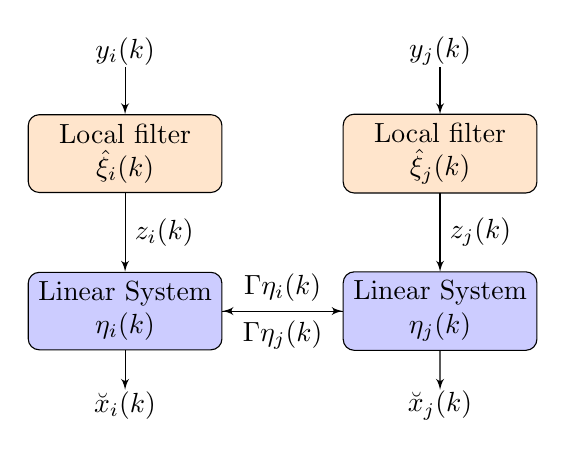
\begin{tikzpicture}[auto, node distance=1.8cm,>=latex']

\node at (0,3.3) {$y_i(k)$};
\node at (4,3.3) {$y_j(k)$};

\draw [->] (0,3.1) -- (0,2.5);
\draw [->] (4,3.1) -- (4,2.5);

\node [sensor,align=center] (est1) {Linear System\\$\eta_{i}(k)$};
\node [sensor, right of=est1,node distance=4cm,align=center] (est2) {Linear System\\$\eta_{j}(k)$};
\node [est,above of=est1,align=center,node distance=2cm] (sensor1) {Local filter\\$\hat{\xi}_i(k)$};
\node [est,above of=est2,align=center,node distance=2cm] (sensor2) {Local filter\\$\hat{\xi}_j(k)$};


\draw [->] (0,1.5) -- node {$z_i(k)$} (0,0.5);
\draw [->] (4,1.5) -- node {$z_j(k)$} (4,0.5);
%\\$y_i(k)$\\\quad\\\quad\\$\hat{\xi}_i(k)$

\draw [->] (est1) -- node {$\Gamma\eta_i(k)$} (est2);
\draw [->] (est2) -- node {$\Gamma\eta_j(k)$} (est1);


\draw [->] (est1) --  (0,-1);
\draw [->] (est2) -- (4,-1);


\node at (0,-1.2) {$\breve{x}_i(k)$};
\node at (4,-1.2) {$\breve{x}_j(k)$};
\end{tikzpicture}
}
    %\caption{The information flow of centralized Kalman filter.}
  \end{figure}
\end{frame}

\begin{frame}{Our algorithm}
  \begin{itemize}
    \item The proposed algorithm yields a \textcolor{thupurple}{stable estimator} at each sensor side as long as the underlying linear system synchronization algorithm is {\bf consistent and exponential stable}:
      \begin{enumerate}
	\item[1)] the average of local estimates from all sensor coincides with the optimal Kalman estimate, namely
	  \begin{equation}
	    \frac{1}{m}\sum_{i=1}^m \breve{x}_i(k)=\hat{x}(k);
	  \end{equation}
	\item[2)] the error covariance of each local estimate is bounded. Moreover, the asymptotic error covariance can be exactly derived.
	\item[3)]  The message being transmitted has a length of $m$, and can be reduced to $n$ if $n<m$.
      \end{enumerate} 
  \end{itemize}
\end{frame}

%	  \begin{frame}{Numerical example}
%	    \begin{columns}[c]
%	      \column{5cm}
%	      \begin{align*}
%		A&=\begin{bmatrix}
%		  0.9 & 0\\
%		  0 & 1.1
%		\end{bmatrix},\\
%		  C&=\begin{bmatrix}
%		    1 & 0\\
%		    0 & 1\\
%		    1 & 1\\
%		    1 & -1
%		  \end{bmatrix},\\
%		    Q&=0.25I_2, R=4I_4.
%		  \end{align*}
%		  \column{7cm}
%		  \begin{figure}
%		    \centering
%		    \includegraphics[width=1\textwidth]{pic/topology.png}
%		    \caption{Topology of the communication graph.}
%		  \end{figure}
%		\end{columns}
%	      \end{frame}
%
%	      \begin{frame}{Simulation result}
%		\begin{figure}
%		  \centering
%		  \scalebox{0.7}{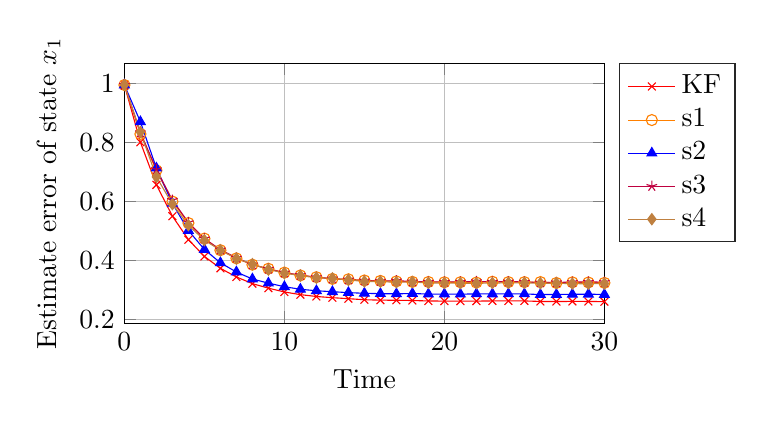
\begin{tikzpicture}
\begin{axis}[%
width=2.4in,
height=1.3in,
scale only axis,
xmin=0,
xmax=30,
xlabel={Time},
ylabel={Estimate error of state $x_1$},
axis background/.style={fill=white},
xmajorgrids,
ymajorgrids,
legend style={legend cell align=left, align=left, draw=white!15!black},
legend pos={outer north east}
]
    \addplot[color={red}, mark={x}]
        coordinates {
            (0,0.9938736998561463)
            (1,0.7998312599375371)
            (2,0.6552675534350793)
            (3,0.5491314278478721)
            (4,0.4694799147910701)
            (5,0.4124624385056815)
            (6,0.3721888244880748)
            (7,0.342896253109788)
            (8,0.32026764135190405)
            (9,0.304892836991136)
            (10,0.29200384686246134)
            (11,0.28297379643031495)
            (12,0.27668961019129906)
            (13,0.2725977233559627)
            (14,0.26926981656843674)
            (15,0.26564889420782367)
            (16,0.2642539514894093)
            (17,0.2639247767173576)
            (18,0.26304078533210873)
            (19,0.26151391429325116)
            (20,0.2610055846609784)
            (21,0.2610801563062564)
            (22,0.26100407922942226)
            (23,0.26165224459393305)
            (24,0.26175778384304416)
            (25,0.26161200966182985)
            (26,0.2598879117677957)
            (27,0.2595078795770665)
            (28,0.26005225008966654)
            (29,0.2598112548773231)
            (30,0.2592574531270815)
            (31,0.2602334111819597)
            (32,0.2608806386097496)
            (33,0.26174960735116337)
            (34,0.26113366656759207)
            (35,0.2599380111371554)
            (36,0.25901760236121385)
            (37,0.25846447356766505)
            (38,0.25883301142410664)
            (39,0.25967947640742967)
            (40,0.25970890124636914)
            (41,0.26073512429871326)
            (42,0.2601919812570974)
            (43,0.2595060207502124)
            (44,0.2599877309012237)
            (45,0.26116255846121617)
            (46,0.2601682050494274)
            (47,0.26074856825442194)
            (48,0.26054896536446837)
            (49,0.2601874302567705)
            (50,0.25943557666834594)
        }
        ;
    \addlegendentry {KF}
    \addplot[color={orange}, mark={o}]
        coordinates {
            (0,0.9938736998561463)
            (1,0.8276013460811993)
            (2,0.7043486327056803)
            (3,0.598584203091598)
            (4,0.5256456013961409)
            (5,0.4730480973677678)
            (6,0.4336170518531029)
            (7,0.4059034949821229)
            (8,0.38459840869216727)
            (9,0.3707972358283984)
            (10,0.3576809276665771)
            (11,0.3481287936793677)
            (12,0.34212296014945826)
            (13,0.3364236636364027)
            (14,0.3350756942959627)
            (15,0.3311186634236469)
            (16,0.32952873899516033)
            (17,0.32796544243410486)
            (18,0.32636001167475454)
            (19,0.3259008402733645)
            (20,0.324931831968992)
            (21,0.32505003087796047)
            (22,0.3240023762232875)
            (23,0.32674547129850556)
            (24,0.32549833224117186)
            (25,0.32541337948482446)
            (26,0.3256170939348204)
            (27,0.32258826225614884)
            (28,0.32475442151198264)
            (29,0.32418172225095204)
            (30,0.3228438634630245)
            (31,0.3245833904161518)
            (32,0.32500396513177804)
            (33,0.3259541718782387)
            (34,0.3254925957091615)
            (35,0.3236953376446919)
            (36,0.32166280136415326)
            (37,0.3239702698216697)
            (38,0.3219689757670435)
            (39,0.323387896278814)
            (40,0.32391586660665317)
            (41,0.3240977569129136)
            (42,0.3260637745636904)
            (43,0.32503775663745)
            (44,0.32551120806489114)
            (45,0.325346440605765)
            (46,0.3248096756157781)
            (47,0.32487774492925325)
            (48,0.3261323039272188)
            (49,0.3235797365529704)
            (50,0.32321206752387277)
        }
        ;
    \addlegendentry {s1}
    \addplot[color={blue}, mark={triangle*}]
        coordinates {
            (0,0.9938736998561463)
            (1,0.8690457045552045)
            (2,0.7119279890009231)
            (3,0.5923819128150415)
            (4,0.5002457913220736)
            (5,0.4361920096215039)
            (6,0.3908883806261038)
            (7,0.35971173152747266)
            (8,0.33586387346463686)
            (9,0.32193945687672326)
            (10,0.3098135515134442)
            (11,0.3011339823202175)
            (12,0.29610710981458166)
            (13,0.29285945258554247)
            (14,0.2897779144208205)
            (15,0.2874991925430223)
            (16,0.28628039600952054)
            (17,0.28568821532927563)
            (18,0.28685086136950994)
            (19,0.28485839609925)
            (20,0.2849303514904291)
            (21,0.28451418544906204)
            (22,0.28550706513452473)
            (23,0.2853174069695211)
            (24,0.2856483722520482)
            (25,0.28536050754699527)
            (26,0.28328233983362844)
            (27,0.2833966472055331)
            (28,0.284043001830299)
            (29,0.28450493552375616)
            (30,0.283564619218778)
            (31,0.28495500414053226)
            (32,0.28530582895421325)
            (33,0.2865198555419734)
            (34,0.285989322134304)
            (35,0.2849749072429814)
            (36,0.28428603282279347)
            (37,0.2822839434538884)
            (38,0.2830552528856996)
            (39,0.28330785066683134)
            (40,0.283483264659842)
            (41,0.2856890215000939)
            (42,0.28421182254422833)
            (43,0.28357028822809305)
            (44,0.28369368444314297)
            (45,0.2850311736621484)
            (46,0.2842881201560302)
            (47,0.28521695596164054)
            (48,0.2847614590394634)
            (49,0.2850139510069791)
            (50,0.28485430954222263)
        }
        ;
    \addlegendentry {s2}
    \addplot[color={purple}, mark={star}]
        coordinates {
            (0,0.9938736998561463)
            (1,0.8325859476122843)
            (2,0.7073897136050656)
            (3,0.6034749935033639)
            (4,0.5275726228149147)
            (5,0.4725831082570765)
            (6,0.43547543835225033)
            (7,0.4078811305071094)
            (8,0.384705576325829)
            (9,0.370092672145898)
            (10,0.3572377352896849)
            (11,0.349201326989582)
            (12,0.3417428545235937)
            (13,0.3373026560410906)
            (14,0.33371971405717166)
            (15,0.33072298139747197)
            (16,0.32873189771116545)
            (17,0.33046645481974085)
            (18,0.32733914555930327)
            (19,0.326086471481113)
            (20,0.32611934637142864)
            (21,0.3264161245451283)
            (22,0.32789165317837493)
            (23,0.32611000923119565)
            (24,0.3270265982465661)
            (25,0.326090148190561)
            (26,0.32373559803173)
            (27,0.3242916189064993)
            (28,0.32542452673580397)
            (29,0.3260128343215159)
            (30,0.3253239754809772)
            (31,0.32603116954327516)
            (32,0.3256400510268415)
            (33,0.3282706785555161)
            (34,0.3260292021373245)
            (35,0.32576855983196407)
            (36,0.3249511540567645)
            (37,0.3230299296021767)
            (38,0.32419268373687665)
            (39,0.32512358156992793)
            (40,0.32661239445773804)
            (41,0.3266854217002811)
            (42,0.3238935627542437)
            (43,0.3229594890948283)
            (44,0.32418033596696927)
            (45,0.32520744181469524)
            (46,0.3249416786945417)
            (47,0.3257839102748252)
            (48,0.32563852090666146)
            (49,0.32690816878238493)
            (50,0.32577337757982483)
        }
        ;
    \addlegendentry {s3}
    \addplot[color={brown}, mark={diamond*}]
        coordinates {
            (0,0.9938736998561463)
            (1,0.8343473999900486)
            (2,0.6822833021672857)
            (3,0.5899142707956274)
            (4,0.5182987446558422)
            (5,0.4675908730658054)
            (6,0.43350277481559124)
            (7,0.40547354140469666)
            (8,0.3862570601591901)
            (9,0.36807970671848506)
            (10,0.3561553044134684)
            (11,0.3471982591140287)
            (12,0.34027389213798453)
            (13,0.3379929251594904)
            (14,0.33278011147647396)
            (15,0.327625385530501)
            (16,0.3270821358208276)
            (17,0.32497323000304207)
            (18,0.32555662692690907)
            (19,0.32276996028079447)
            (20,0.32215457434325434)
            (21,0.3217828459857988)
            (22,0.3213620072692803)
            (23,0.32229698073255747)
            (24,0.3229285159012965)
            (25,0.32293444859886605)
            (26,0.3214561133226882)
            (27,0.3216030504550832)
            (28,0.32021398223117714)
            (29,0.31985569158716703)
            (30,0.3205502791012525)
            (31,0.32073406012314265)
            (32,0.3219379552948372)
            (33,0.32103738203264903)
            (34,0.32159115134826693)
            (35,0.31934458799994936)
            (36,0.3205593093017057)
            (37,0.31870880349791386)
            (38,0.32081053658788317)
            (39,0.3218149433555171)
            (40,0.3197246279159553)
            (41,0.3211652693961577)
            (42,0.32126305883557493)
            (43,0.3211102597500812)
            (44,0.3204900260033881)
            (45,0.323094674930004)
            (46,0.32125045787242584)
            (47,0.3212528756591601)
            (48,0.32056885659423623)
            (49,0.320213202267437)
            (50,0.31999954839432815)
        }
        ;
    \addlegendentry {s4}
\end{axis}
\end{tikzpicture}
}
%		  \scalebox{0.7}{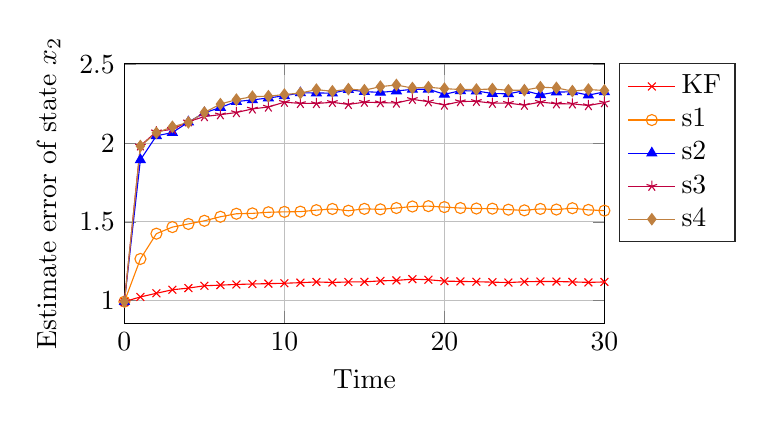
\begin{tikzpicture}
\begin{axis}[%
width=2.4in,
height=1.3in,
scale only axis,
xmin=0,
xmax=30,
xlabel={Time},
ylabel={Estimate error of state $x_2$},
axis background/.style={fill=white},
xmajorgrids,
ymajorgrids,
legend style={legend cell align=left, align=left, draw=white!15!black},
legend pos={outer north east}
]
    \addplot[color={red}, mark={x}]
        coordinates {
            (0,0.9943765995349962)
            (1,1.0241254689704056)
            (2,1.0473887499847159)
            (3,1.0697339448807577)
            (4,1.0803713746007921)
            (5,1.0949033915033333)
            (6,1.0991482380149056)
            (7,1.1034194862558937)
            (8,1.106307793947288)
            (9,1.1085925380380288)
            (10,1.110999599114129)
            (11,1.1147645806759343)
            (12,1.1193703731575648)
            (13,1.116094933319016)
            (14,1.1192249437084907)
            (15,1.1199115573191498)
            (16,1.1260096469155687)
            (17,1.1291450572405135)
            (18,1.136950337574846)
            (19,1.133455361109355)
            (20,1.1244685761514959)
            (21,1.1227919434732434)
            (22,1.1206090843375092)
            (23,1.1180481048662483)
            (24,1.1155404791626586)
            (25,1.1204428581200438)
            (26,1.1224462151114232)
            (27,1.121752685683367)
            (28,1.1196943320049257)
            (29,1.1164613963806695)
            (30,1.1193740859610601)
            (31,1.1196678829620261)
            (32,1.1262821415531057)
            (33,1.1156317612924114)
            (34,1.116567512625055)
            (35,1.116742559368047)
            (36,1.117315577996865)
            (37,1.118028323124454)
            (38,1.1164678892437345)
            (39,1.117983506365516)
            (40,1.123098865189546)
            (41,1.1230946876927135)
            (42,1.1225522521222113)
            (43,1.1224618836995262)
            (44,1.1238984888915637)
            (45,1.125901217233803)
            (46,1.1226315332791659)
            (47,1.119965687831627)
            (48,1.1193711594564655)
            (49,1.1226049410413392)
            (50,1.1241068397421996)
        }
        ;
    \addlegendentry {KF}
    \addplot[color={orange}, mark={o}]
        coordinates {
            (0,0.9943765995349962)
            (1,1.2652924039335356)
            (2,1.4256320040837056)
            (3,1.4673510411562172)
            (4,1.4873395687011577)
            (5,1.5073301774920105)
            (6,1.5329161641112685)
            (7,1.5520030589757723)
            (8,1.554391863843294)
            (9,1.5615200183722036)
            (10,1.563923717117754)
            (11,1.5653870801152323)
            (12,1.574879924241972)
            (13,1.5825303535941295)
            (14,1.5711163184525245)
            (15,1.5831105788545525)
            (16,1.5799868657614462)
            (17,1.5882189783567848)
            (18,1.5979613761646876)
            (19,1.6003075631065073)
            (20,1.5941329592447682)
            (21,1.588284581504355)
            (22,1.5851274627279721)
            (23,1.584373968832322)
            (24,1.577858666299255)
            (25,1.5735674219348068)
            (26,1.5827615472696204)
            (27,1.5786961819804337)
            (28,1.587122886228931)
            (29,1.5765449008480295)
            (30,1.571758603170185)
            (31,1.5722071728043354)
            (32,1.5790341798123353)
            (33,1.5937749764613511)
            (34,1.5745873058034463)
            (35,1.5701470146906793)
            (36,1.5669255079112894)
            (37,1.5699117333623531)
            (38,1.57213903822218)
            (39,1.5750483423635424)
            (40,1.5761992587434166)
            (41,1.5812174368332743)
            (42,1.5817244605547665)
            (43,1.586364793112144)
            (44,1.5853213582576369)
            (45,1.5866770960927927)
            (46,1.5821300768923279)
            (47,1.5851061919445362)
            (48,1.5826051452764909)
            (49,1.572164251666703)
            (50,1.5822951282611506)
        }
        ;
    \addlegendentry {s1}
    \addplot[color={blue}, mark={triangle*}]
        coordinates {
            (0,0.9943765995349962)
            (1,1.8936625444249422)
            (2,2.0465205257360233)
            (3,2.066951276012711)
            (4,2.1338615693851746)
            (5,2.1922909740541803)
            (6,2.226487115248709)
            (7,2.263933580097268)
            (8,2.2742324432017647)
            (9,2.2866612655231235)
            (10,2.300561709236413)
            (11,2.3187874391349936)
            (12,2.3183107436885133)
            (13,2.3172153186124294)
            (14,2.339358433536219)
            (15,2.326601894094998)
            (16,2.322100645625816)
            (17,2.3311028833616803)
            (18,2.3412621523512342)
            (19,2.342196254698138)
            (20,2.309811332436182)
            (21,2.3326324701167347)
            (22,2.331147100728079)
            (23,2.314863629664187)
            (24,2.31285475802809)
            (25,2.3332171428385466)
            (26,2.3071309244263793)
            (27,2.3241146984247614)
            (28,2.3254061798842365)
            (29,2.304722589550026)
            (30,2.3250475757893168)
            (31,2.326875039249452)
            (32,2.347786042018165)
            (33,2.3050612298653994)
            (34,2.3143523106351727)
            (35,2.323050036506524)
            (36,2.3268902505681694)
            (37,2.326027817270796)
            (38,2.3264477462757323)
            (39,2.3118714464205596)
            (40,2.329829962182898)
            (41,2.313641678866345)
            (42,2.334185411755957)
            (43,2.3313963439610914)
            (44,2.319456118549934)
            (45,2.3358929879940047)
            (46,2.3168383584104326)
            (47,2.321115857214799)
            (48,2.3270072795412897)
            (49,2.3384601141712515)
            (50,2.318873680806025)
        }
        ;
    \addlegendentry {s2}
    \addplot[color={purple}, mark={star}]
        coordinates {
            (0,0.9943765995349962)
            (1,1.9828858762138304)
            (2,2.072953590569488)
            (3,2.0880223184728335)
            (4,2.1360134385063105)
            (5,2.168877836105569)
            (6,2.180518305551039)
            (7,2.194470270203278)
            (8,2.2170095545654873)
            (9,2.2294796048964476)
            (10,2.259813698050696)
            (11,2.252040729684584)
            (12,2.2518134092075446)
            (13,2.258969773117035)
            (14,2.2456372378476983)
            (15,2.260074704840985)
            (16,2.25690801887656)
            (17,2.2546645079335232)
            (18,2.2780084217125545)
            (19,2.2627407160130613)
            (20,2.241840788498835)
            (21,2.2639896937363018)
            (22,2.2653910716270422)
            (23,2.253397842090359)
            (24,2.253664694284399)
            (25,2.2409423831703603)
            (26,2.260721382240181)
            (27,2.2498742978256083)
            (28,2.249337306194815)
            (29,2.2387064936893575)
            (30,2.2572354436442903)
            (31,2.2559199593761075)
            (32,2.2629454575339145)
            (33,2.237792912635502)
            (34,2.259809633090449)
            (35,2.2600701221241586)
            (36,2.2590233377061026)
            (37,2.2566562394095957)
            (38,2.259200706317603)
            (39,2.2522596098668717)
            (40,2.271687711433266)
            (41,2.251367671607407)
            (42,2.2467096704728404)
            (43,2.2653285924423328)
            (44,2.249874385082106)
            (45,2.2693838984464265)
            (46,2.2443897174131746)
            (47,2.2700278666501776)
            (48,2.2596714046786364)
            (49,2.2710007617069685)
            (50,2.2585889284508913)
        }
        ;
    \addlegendentry {s3}
    \addplot[color={brown}, mark={diamond*}]
        coordinates {
            (0,0.9943765995349962)
            (1,1.9816540696459648)
            (2,2.0654615474192903)
            (3,2.1035165609535103)
            (4,2.1315441874490997)
            (5,2.194405042764902)
            (6,2.2477131762354583)
            (7,2.2761788789650046)
            (8,2.2947881679581665)
            (9,2.2977677725464183)
            (10,2.308375957467222)
            (11,2.317980480162738)
            (12,2.339427607324274)
            (13,2.32883551380075)
            (14,2.3427375592794983)
            (15,2.3356439111894307)
            (16,2.3585557228897294)
            (17,2.3690788525616533)
            (18,2.3493756113388495)
            (19,2.354762160569893)
            (20,2.3456192480187106)
            (21,2.3403966321669003)
            (22,2.340282752809893)
            (23,2.3432582094375234)
            (24,2.3354632251712575)
            (25,2.3358984300908086)
            (26,2.3548376694214577)
            (27,2.350751598558515)
            (28,2.330001313064622)
            (29,2.339936620551301)
            (30,2.334139579826345)
            (31,2.3296671247918894)
            (32,2.3477739816701084)
            (33,2.3372527594188757)
            (34,2.3294471328167496)
            (35,2.331507818950099)
            (36,2.3364833657462096)
            (37,2.3324300667271194)
            (38,2.3362024692199643)
            (39,2.3484213589008274)
            (40,2.332847142957334)
            (41,2.3589948008145787)
            (42,2.345722793829973)
            (43,2.3270312885418902)
            (44,2.3439433888447985)
            (45,2.3273308186147994)
            (46,2.36039655167833)
            (47,2.339409769673635)
            (48,2.336415886140528)
            (49,2.3442896822054715)
            (50,2.328126528073856)
        }
        ;
    \addlegendentry {s4}
\end{axis}
\end{tikzpicture}
}
%		  \caption{Average mean square estimation error of state estimates under Kalman filter and local estimators in 10000 experiments.}
%		\end{figure}
%	      \end{frame}
%
%	      \begin{frame}{Numerical example}
%		We simulate the heat transfer process in a planar closed region:
%		\begin{align*}
%		  \frac{\partial u}{\partial t}=\alpha\Big(\frac{\partial^2u}{\partial x_1^2}+\frac{\partial^2u}{\partial x_2^2}\Big),
%		\end{align*}
%		with boundary conditions
%		\begin{align*}
%		  \frac{\partial u}{\partial x_1}\Big|_{t,0,x_2}=\frac{\partial u}{\partial x_1}\Big|_{t,l,x_2}=\frac{\partial u}{\partial x_2}\Big|_{t,x_1,0}=\frac{\partial u}{\partial x_2}\Big|_{t,x_1,l}=0,
%		\end{align*}
%	      \end{frame}
%
%	      \begin{frame}{Simulation result}
%		\begin{figure}[]
%		  \centering
%		  \includegraphics[width=0.6\textwidth]{pic/variance.pdf}
%		  \caption{(a) Position and topology of $m$ sensors; (b) Centralized KF; (c) Local KF; (d) Our estimators in 10000 experiments.}
%		  \label{fig:heatmap}
%		\end{figure}
%	      \end{frame}
%
%	      \begin{frame}{Equipments}
%		\begin{columns}[c]
%		  \column{6cm}
%		  \begin{itemize}
%		    \item Hardware: 30 raspberry pis, power banks and sensors.
%		    \item Software: batman-adv.
%		      \begin{itemize}
%			\item Operates entirely on layer 2.
%			\item Supports 1000 nodes and beyond.
%		      \end{itemize}
%		    \item Goal: build a mesh network and perform various distributed tasks.
%		  \end{itemize}
%		  \column{6cm}
%		  \begin{figure}
%		    \centering
%		    \includegraphics[width=0.6\textwidth,angle=90]{pic/rapberry_pi.jpg}
%		    \caption{Available equipments.}
%		  \end{figure}
%		\end{columns}
%	      \end{frame}
%
%	      \begin{frame}{Batman-adv}
%		\begin{figure}
%		  \centering
%		  \includegraphics[width=0.7\textwidth]{pic/batman-adv.png}
%		  \includegraphics[width=0.5\textwidth]{pic/batman-topology.png}
%		  \caption{Build mesh networks with batman-adv.}
%		\end{figure}
%		Future work:
%		\begin{itemize}
%		  \item Find ways to determine the topology.
%		  \item Time synchronization.
%		  \item Create a tool to visualize and monitor.
%		\end{itemize}
%	      \end{frame}

\begin{frame}{Experiment with Raspberry Pis}
  \begin{columns}[c]
    \column{7cm}
    \begin{itemize}
      \item A mesh network is created over WiFi with batman-adv.
      \item Batman wireless routing protocol enables each Raspberry Pi to find and communicate with its neighbors in an {\bf ad-hoc} fashion.
    \end{itemize}
    \column{5cm}
    \begin{figure}
      \centering
      \includegraphics[width=1\textwidth]{pic/rpi_expriment.png}
    \end{figure}
  \end{columns}
\end{frame}

%	      \begin{frame}{Experiment with Raspberry Pis}
%		\begin{columns}[c]
%		  \column{7cm}
%		  \begin{itemize}
%		    \item Raspberry Pis send messages with ZeroMQ \cite{ZeroMQ}, an open-source universal messaging library.
%		    \item ZeroMQ is aimed at use in distributed or concurrent applications and supports many patterns (pub/sub, request/reply, client/server etc.)
%		  \end{itemize}
%		  \column{5cm}
%		  \begin{figure}
%		    \centering
%		    \includegraphics[width=1\textwidth]{pic/msg.png}
%		  \end{figure}
%		\end{columns}
%	      \end{frame}

\begin{frame}{Experiment}
  We simulate the heat transfer process in a planar closed region:
  \begin{align*}
    \frac{\partial u}{\partial t}=\alpha\Big(\frac{\partial^2u}{\partial x_1^2}+\frac{\partial^2u}{\partial x_2^2}\Big),
  \end{align*}
  with boundary conditions
  \begin{align*}
    \frac{\partial u}{\partial x_1}\Big|_{t,0,x_2}=\frac{\partial u}{\partial x_1}\Big|_{t,l,x_2}=\frac{\partial u}{\partial x_2}\Big|_{t,x_1,0}=\frac{\partial u}{\partial x_2}\Big|_{t,x_1,l}=0.
  \end{align*}
  Sensors are randomly deployed in this region. With a grid and fixed sample frequency, the process can be discretized as:
  \begin{align*}
    U(k+1)&=AU(k)+w(k)\\
    Y(k)&=CU(k)+v(k).
  \end{align*}
\end{frame}

\begin{frame}{Experiment result}
  \begin{figure}[]
    \centering
    \includegraphics[width=0.65\textwidth]{pic/variance.pdf}
  \end{figure}
\end{frame}

\section{Conclusion}

\begin{frame}{Conclusion}
  \begin{itemize}
    \item We presented a way to decompose a steady-state Kalman filter into {\bf local filters} and a {\bf global weighted sum}
    \item By replacing the sum with LASSO, we can derive a secure version of the Kalman filter, with minimum loss of performance
    \item By replacing the sum with a linear system synchronization algorithm, we provide a framework for distributed estimation.
  \end{itemize}
\end{frame}

\begin{frame}{Reference}

  [1] Xinghua Liu, Yilin Mo and Emanuele Garone, Local Decompostion of Kalman Filters and Its Application for Secure State Estimation, IEEE Transactions on Automatic Control, Accepted

  [2] J. Yan, X. Yang, Y. Mo, and K. You. ``A distributed implementation of steady-state Kalman filter'', IEEE Transactions on Automatic Control, submitted

  \vspace{10pt}
  \centering
  \includegraphics[width=0.3\textwidth]{pic/qr.jpeg}
\end{frame}


\begin{frame}[standout]
  Thank you for your time! 
\end{frame}

\end{document}

